%This is a comment, it will not be compiled...

\listfiles
\documentclass[12pt]{report} 
%%nomenclature hack from http://www.freiheitsfreund.de/2010/10/24/automatically-run-makeindex-from-within-a-latex-document-with-write18/%%%

\usepackage[intoc]{nomencl}

\textwidth=6in \oddsidemargin=0.5in \topmargin=-0.5in
\textheight=9in  % 9in must include page numbers
\textfloatsep = 0.4in \addtocontents{toc}{\vspace{0.4in} \hfill
Page\endgraf} \addtocontents{lof}{\vspace{0.2in} \hspace{0.13in} \
Figure\hfill Page\endgraf} \addtocontents{lot}{\vspace{0.2in}
\hspace{0.13in} \ Table\hfill Page\endgraf}

\usepackage[export]{adjustbox}
\usepackage[T1]{fontenc}
\usepackage{textcomp}
\usepackage{array}
\usepackage{listings}
\usepackage{tabularx}
\usepackage{setspace}
\usepackage{mathptmx}
\usepackage[table, svgnames]{xcolor}
\usepackage{colortbl}
\usepackage{graphicx}
\usepackage{amssymb, amsmath}
\usepackage{subfig}
\usepackage{epsfig}
\usepackage{times}
\usepackage{float}
\usepackage{pbox}
\usepackage{rotating}
\usepackage{makeidx}
\usepackage{url}
\usepackage{multirow}
\usepackage{booktabs}
\usepackage[subfigure, titles]{tocloft}
\usepackage[printonlyused,withpage]{acronym}
\usepackage{datetime}
\usepackage{fancyvrb}
\usepackage{color}
\usepackage[autostyle,english=american]{csquotes} 
\usepackage{wrapfig}
\MakeOuterQuote{"}
%%another algorithm package
\usepackage{algorithm}
\usepackage{algorithmic}

%\renewcommand{\nomname}{LIST OF ABBREVIATIONS}
%\makenomenclature

\graphicspath{{images/intro/}}
\DeclareGraphicsExtensions{.pdf,.jpeg,.png,.PNG, .eps, .tiff}

\urlstyle{same}

\usepackage{makecell}
\usepackage{titletoc}
\usepackage{sfchap}
\usepackage{sfsection}
\usepackage[authoryear]{natbib}
%\usepackage{apacite}
\usepackage{appendix}
%\usepackage{tocbibind}
%
\usepackage[nottoc]{tocbibind}
\setcounter{secnumdepth}{7}
\setcounter{tocdepth}{7}

\usepackage{hyperref}
\hypersetup{
	pdftitle={Rational Design of Antibodies: From Mechanisms of Specificity to Novel Vaccine Strategies},
	pdfauthor={Jordan Willis},
	bookmarksnumbered, %Determined if chapter numbers are included in the bookmark list
	pdfstartview={FitH},
	pdfborder={0 0 0},
	plainpages=false
}%
\usepackage[all]{hypcap}

% Stats table label
\newcommand{\statslabel}[2]{\multirowcell{#1}[-1.6mm][c]{#2}}

% Below heading rule.
\newcommand{\otoprule}{\midrule[\heavyrulewidth]}

% Prevent double spaced equations
\newenvironment{tightequation}{\singlespace\begin{equation}}{\end{equation}}

% Extra junk to pretty up the table of contents
\setlength{\cftsecnumwidth}{2.8em}
\setlength{\cftsubsecnumwidth}{3.7em}
\setlength{\cftsubsubsecnumwidth}{4.6em}
\setlength{\cftparanumwidth}{5.5em}
\setlength{\cftsubparanumwidth}{6.5em}
\setlength{\cfttabnumwidth}{3.5em}
\setlength{\cftfignumwidth}{3.5em} 

\renewcommand{\contentsname}{TABLE OF CONTENTS}
\renewcommand{\listfigurename}{LIST OF FIGURES}
\renewcommand{\listtablename}{LIST OF TABLES}
\renewcommand{\bibname}{ \texorpdfstring{{BIBLIOGRAPHY\vspace{10mm}}}{BIBLIOGRAPHY}   }
%
\renewcommand{\chaptermark}[1]{%
  \markboth{\MakeUppercase{%
      \chaptername}\ \thechapter.%
    \ #1}{}}
    
    
\interfootnotelinepenalty=10000 %prevents the splitting of long footnotes across multiple pages. Use with caution. 

%%Put useful shortcuts here:

\newcommand{\ki}{K$_{i}$}
\newcommand{\ic}{IC$_{50}$}
\begin{document}

%%%%%%%%%%%%%%%%%%%%%%%%%%%%%%%%%%%%%%%%%%%%%%%%%%%%%%%%%%%%%%%%%%%%%%%%%%%%%%%%
%% Prevent the warning: pdfTeX warning (ext4): destination with the same identifier (name{page.1}) has been already used, duplicate ignored
%%	This setting will make a difference to the output because the page number is suppressed for the title page
\pagenumbering{alph}

\begin{titlepage}
\thispagestyle{empty}\enlargethispage{\the\footskip}%
\begin{center}
	{\setstretch{1.66} \MakeUppercase{Rational Design of Antibodies: From Mechanisms of Specificity to Novel Vaccine Strategies}\par }%
	\vskip.3in
	By
	\vskip .3in
	{Jordan  R. Willis}
	\vskip .3in
	
	\begin{doublespace}
		Dissertation\\
		Submitted to the Faculty of the \\
		Graduate School of Vanderbilt University \\
		in partial fulfillment of the requirements \\
		for the degree of \\ [.2in]
	\end{doublespace}
	
	\MakeUppercase{Doctor of Philosophy} \\[.1in]
	in \\[.2in]
	\MakeUppercase{Chemical and Physical Biology} \\[.25in]
	August,\space\number\year \\[.45in]
	Nashville, Tennessee
	\vskip .5in
\end{center}

\newcommand*{\SignatureAndDate}[1]{%
    \setlength{\parskip}{0cm}
    \par\noindent\makebox[3.5in]{\hrulefill} \hfill\makebox[2.0in]{\hrulefill}%
    \par\noindent\makebox[3.5in][l]{#1}      \hfill\makebox[2.0in][l]{}%
   \\[0.15in]%
}%

%%%Uncomment for Signatures%%%
%Approved: \hskip 2.9in Date:\\[1.2em]
%\rule{3.5in}{.5pt} \hskip 0.1in \rule{2in}{.5pt} \\[.2in]
%\rule{3.5in}{.5pt} \hskip 0.1in \rule{2in}{.5pt} \\[.2in]
%\rule{3.5in}{.5pt} \hskip 0.1in \rule{2in}{.5pt} \\[.2in]
%\rule{3.5in}{.5pt} \hskip 0.1in \rule{2in}{.5pt} %\\[.1in]
%%%%%%%%%%%%%%
%%%%%%Uncomment  for Approved Names%%%%%%
\begin{center}
\begin{singlespace}
Approved: \hskip 2.9in Date:\\[1.2em]
\SignatureAndDate{Benjamin Spiller, Ph.D (Chair)}
\SignatureAndDate{Christopher Aiken, Ph.D}
\SignatureAndDate{Jens Meiler, Ph.D}
\SignatureAndDate{Spyros Kalams, M.D.}
\SignatureAndDate{James Crowe, M.D.}
\end{singlespace}
\end{center}
\end{titlepage}

%%%%%%%%%%%%%%%%%%%%%%%%%%%%%%%%%%%%%%%%%%%%%%%%%%%%%%%%%%%%%%%%%%%%%%%%%%%%%%%%
\doublespacing
\pagenumbering{roman} \setcounter{page}{1}
 

%\chapter*{Acknowledgements}
\addcontentsline{toc}{chapter}{Acknowledgements}
\vspace{7mm}
This work would not have been possible without the following people.
First and foremost, I would like to thank my two mentors, James Crowe and Jens Meiler. The general consensus of the biomedical science community is that principal investigators often dislike interdepartmental collaboration. When I talk to other graduate students, I find that they have many unpleasant experiences with just a single investigator. I feel very fortunate to have two PIs with whom I get along so well. From opposite ends of the spectrums of science, they never objected to such a collaboration. Were it only a few years ago this feat may have been unattainable. Both of you are an inspiration to my scientific future. Jens with his incredible and often frustrating brilliance of the task at hand, and Jim with his scientific leadership. I could not have asked for two better bosses to nurture my scientific growth.

I would lake to thank all my colleagues in the Crowe and Meiler Labs. An early thanks goes to Kristian Kaufmann, Ralf Mueller, and Mark Hicar, as their initial guidance through my rotation was a deciding factor in my choice for the future. There are innumerable scientific colleagues who helped me with my work including Jessica Finn who helped with the high-throughput sequencing, Mark Hicar who taught me about HIV virology, Sam DeLuca who would answer every question I had about computers, Gordon Lemmon who taught me scripting, Steven Combs who guided me through \rosetta, and Natalie Thornburg for teaching me many molecular biology techniques. I would also like to thank the lab technicians who made this throughput of work possible, Rachelle Falk, Vidisha Singh, and Hannah King. Special thanks go to a dear friend and brilliant scientist Gopal Sapparapru. Your troubleshooting techniques, management of large amounts of experimental data, and guidance through countless experiments has helped make me a better scientist. I would like to make a very special mention to my very good friend and colleague Bryan Briney, who taught me almost everything I know about immunology and high-throughput sequencing. Our names appear together on many publications for good reason.

I want to thank my friends and family. Graduate school is a long arduous process and without them I would not be where I am today. First, my sister, who I cannot live up to. You have a heart of gold. My Mother, my number one fan. Her constant encouragement has helped me survive graduate school. I'm lucky to have her in my life and to have spent a majority of my time in Nashville with her close. She is a great source of inspiration in all that I do. A constant drive and loving force. My Father, my role model. His support for me has been tremendous. His drive and motivation showed me what a little hard work can do. I hope to become half of the man he is today. My friends, helping me keep sanity through graduate school. I would especially like to thank Sean Welch, who allowed me sanctuary away from graduate school. You are also a tremendous inspiration. Lastly I would like to thank my best friend in graduate school, my cat Ocho, the only constant through these last six years. I love you little buddy! Here's to many more years together.

%\chapter*{Summary}
\addcontentsline{toc}{chapter}{Summary}
\vspace{7mm}
This document is the culmination of my work on antibody design. Primarily, my target system is HIV with some work on Influenza. It is divided up into orthogonal publications, with each publication having incorporated an aspect of antibody design. Here I use the modeling suite \rosetta~whenever I mention \silico~solutions to design problems. All computational work was done by me as well as validation with the experimental characterization.

The introduction in chapter \ref{chap:chapter1} outlines four pieces of background knowledge that must be considered for the remaining chapters to become clear. I first detail antibodies in general, as this document only considers immunoglobulins as the design target of interest. I detail their purpose and how they are diversified to create an immunoglobulin repertoire. I next detailed the pandemic of HIV, its structure, and the current state of an efficacious vaccine, and describe the broadly neutralizing antibodies that have been characterized to date. I also describe the molecular modeling suite \rosetta~and briefly cover the \rosetta~energy function. I detail a particular application in \rosetta~known as \rosettadesign, which is the focus of my thesis. I then describe how \rosettadesign~has been used in translational medicine. Lastly I detail the current state of the field, the difficulties in molecular modeling, the challenges in protein design, and how this work can be used to aid in these challenges. Briefly, I describe how antibody design is used to answer questions about basic science to implications for vaccine strategies. It is here that I tie antibody design with all aspects of my research.

The beginning of my research starts in chapter \ref{chap:chapter2}. This part of my research aims to answer a basic question in immunology. Here I used \rosettadesign~to investigate the molecular basis for polyspecificity. It is known that a finite set of antibodies is able to accommodate a nearly limitless antigen space. Using design, I investigated which sequences are ideal to bind multiple antigens or single antigens in a protocol I used called multi-state design.

Using the strategies and principles built upon in chapter \ref{chap:chapter2}, chapter \ref{chap:chapter3} focuses on a novel vaccine paradigm. Here I used antibody design to interrogate the HIV-\naive~donor antibody repertoire with a simple goal in mind: Does the HIV-\naive~antibody repertoire contain antibodies that resemble known broadly neutralizing antibodies? This paradigm focuses on a structural mimicry rather than a sequence identity, which not only allows me to use \rosettadesign~and homology modeling as a tool to investigate this hypothesis, but mandates it, showing the necessity of molecular modeling. All antibodies found in this chapter were made experimentally and characterized to corroborate computational findings.

In chapter \ref{chap:chapter4}, I used \rosettadesign~to show that the antibody PG9, which is known to be one of the most broad and potent antibodies against HIV-1 characterized to date, still has room for improvement. Mutations were returned from \rosettadesign~which were predicted to enhance breadth and specificity. These mutations were tested experimentally and did indeed corroborate our hypothesis that even the most broad and potent antibodies could be improved with careful computational design and analysis.

Finally, chapter \ref{chap:chapter5} details future directions I foresee for these project. These strategies are generalizable and can be applied to any given antibody/antigen system and may even extend to any given protein-protein interface. In addition, I consider reasons for design failures, imperfect sequence recovery, and antibodies that failed to corroborate \silico~predictions. I give an idea of many future experiments that could be used to take of advantage of the information detailed in this document. I also detail  some of my other work on viral escape assessed by computational modeling and broadly neutralizing mAbs to Influenza which were in various stages of completion.

\singlespacing
\tableofcontents

%%%%%%%%%%%%%%%%%%%%%%%%%%%%%%%%%%%%%%%%%%%%%%%%%%%%%%%%%%%%%%%%%%%%%%%%%%%%%%%%
\begingroup
\setlength{\parskip}{1\baselineskip}
\listoftables
\newpage
\listoffigures
\newpage
%\chapter*{LIST OF ABBREVIATIONS}
\addcontentsline{toc}{chapter}{LIST OF ABBREVIATIONS}
\vspace{7mm}
\begin{acronym}[ROC-AUC]
\acro{ANN}{Artificial Neural Network}
\acro{BCL}{BioChemical Library}
\acro{BLAST}{Basic Local Alignment Search Tool}
\acro{CASP}{Critical Assessment of protein Structure Prediction}
\acro{CPU}{Central Processing Unit}
\acro{CSAR}{Community Structure-Activity Resource}
\acro{CSV}{Comma Separated Value}
\acro{DBN}{Deep Belief Network}
\acro{FPR}{False Positive Rate}
\acro{GOLD}{Genetic Optimization of Ligand Docking}
\acro{GPCR}{G-Protein Coupled Receptor}
\acro{GPU}{Graphical Processing Unit}
\acro{HSE}{Half Sphere Exposure}
\acro{JSON}{JavaScript Object Notation}
\acro{KBP}{Knowledge-Based Potential}
\acro{LGA}{Lamarckian Genetic Algorithm}
\acro{MCM}{Monte Carlo Minimization}
\acro{MIN}{Minimization}
\acro{NCR}{Neighbor Count}
\acro{NR}{Non-Redundant}
\acro{NV}{Neighbor Vector}
\acro{ORM}{Object-Relational Mapping}
\acro{PBS}{Portable Batch System}
\acro{PDB}{Protein DataBank}
\acro{PPV}{Positive Predictive Value}
\acro{PSSM}{Position Specific Scoring Matrix}
\acro{QSAR}{Quantitative Structure Activity Relationship}
\acro{RDF}{Radial Distribution Function}
\acro{RMS}{Root Mean Square}
\acro{RMSD}{Root Mean Square Deviation}
\acro{ROC}{Receiver Operating Characteristic}
\acro{ROC-AUC}{Receiver Operating Characteristic Area Under Curve}
\acro{rSASA}{relative Solvent Accessible Surface Area}
\acro{SASA}{Solvent Accessible Surface Area}
\acro{SCOP}{Structural Classification of Proteins}
\acro{SDF}{Structure Data File}
\acro{SQL}{Structured Query Language}
\acro{TPR}{True Positive Rate}
\acro{vHTS}{virtual High Throughput Screening}
\acro{WNCR}{Weighted Neighbor Count}
\acro{XML}{Extensible Markup Language}
\end{acronym}
 %table of acronymns
\newpage
\endgroup

%%%%%%%%%%%%%%%%%%%%%%%%%%%%%%%%%%%%%%%%%%%%%%%%%%%%%%%%%%%%%%%%%%%%%%%%%%%%%%%%
\normalsize
\doublespacing
\pagenumbering{arabic}
\setcounter{page}{1}

%In addition you need a substantial (10-20 pages) introductory chapter detailing
%  Significance (Why was the research done needed) and
%  Innovation (Why was the research done novel? How does it relate to competing methods?) of the body of work in your thesis.
%This chapter could ideally come form a review article you have written.
\chapter{Introduction}
\label{chap:introduction}
\section{Antibody Overview}
The lymphocytes that make up the adaptive immune system have evolved to recognize a limitless number of antigens that constitute viruses, bacteria and all foreign material to a hosts immune system  \citep{Murphy:2007tl}. The concern of this thesis is on the antigen-recognition molecules of the B-cell known as immunoglobulins (Ig). These can exists either as a membrane-anchored form to the B-cell known as the B-cell receptor (BCR) or as a secreted form with a wide range of functionality known as the antibody. The main effector function of the antibody is to bind foreign pathogens in the body and is the basis for the adaptive immune response. The antibody molecule has two separate functions. One is to bind specifically to molecules known as antigens. The other is to recruit other cells and molecules to destroy the pathogens each immunoglobulin is bound to. There are two genetic domains that make up the antibody structure and differentiate these processes (figure \ref{fig:antibodyoverview}). One is the variable domain responsible for specificity. The other is the constant domain that engages different effector functions such as cytokine recruitment and phagocytosis of compromised cells. Structurally, antibodies consist of two identical heavy chains, that are recombined gene segments of the heavy variable and constant domain gene segments, and two identical light chains, which are recombined copies of light chain variable and constant domains gene segments.

The variability of the antibody molecule is what ensures that any individual with a functional immune system can produce an antibody to recognize almost any structure. The mechanisms of variability are discussed in further sections but are typically distributed to the apical tips of the antibody structure. It is important to note that the B-cell bound receptor and effector function of antibodies play an important role in the humoral immune system, but the remainder of this document will focus on the diversity and specificity of secreted antibodies of the IgG class, the most common circulating immunoglobulin.  

\begin{figure}%Antibody Structure
\centering
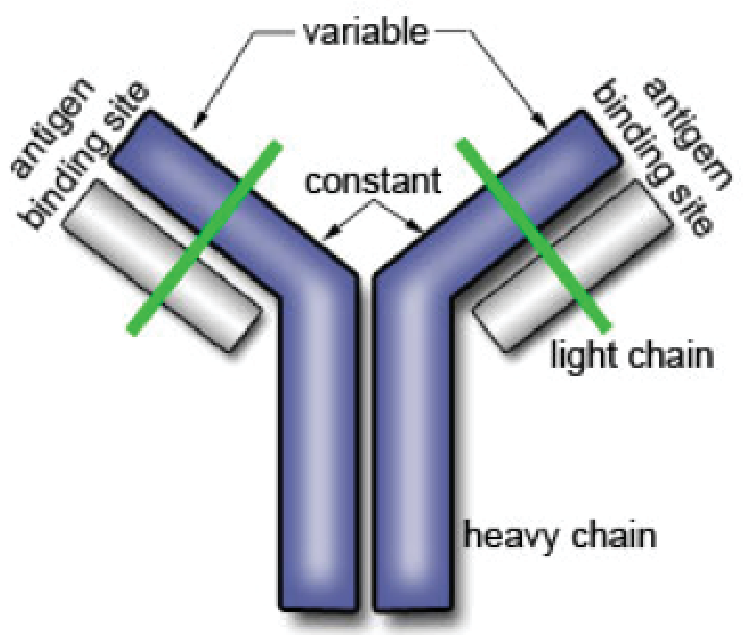
\includegraphics[width=.45\textwidth]{images/intro/figure1_1.pdf}
\caption[Overview of Antibody Structure]{
Overview of Antibody Structure. Heavy chain is shown in blue, light chain in grey. The structure is divided into the variable portion responsible for recognition, and the constant portion responsible for effector function. The apical tips of the antibodies are where antigens typically bind and are therefore known as the antigen binding sites. Image reproduced from http://crdd.osdd.net/raghava/absource/abasic.html.
}
\label{fig:antibodyoverview}
\end{figure}

\subsection{Antibody Diversification}
The antibody genes that encode heavy and light chains are located in three primary locations in the human genome: heavy chain genes (IGH) are located on chromosome 14, light chain kappa genes (IGK) are located on chromosome 2, and light chain lambda genes (IGK) are located on chromosome 22 \citep{Brochet:2008kq}. Each of these loci consists of multiple variable (V, not to be confused with the variable region of an antibody) and joining (J) gene segments. In addition the IGH locus also contains several diversity (D) gene segments.  Sequencing of the human IGH locus revealed 55 functional V genes, 23 D genes, and six J genes \citep{Matsuda:1998ua,Lefranc:2009ga}. The human variable genes (and, at the IGH locus, the diversity genes) can be phylogenetically grouped into families based on sequence similarity. Heavy chain variable genes are organized into seven families and homology within gene families is typically above 80\%. The 23 functional human diversity genes are also organized into seven families. An example variable gene, IGVH5-15*01, the standard IMGT nomenclature for human V and D genes follows the following pattern: the chain and gene description (IGHV for variable genes, IGHD for germline genes), the family, the gene number (determined by position in the germline locus), and the allele. The gene number is separated from the family with a hyphen and the allele is separated from the gene number with an asterisk.


\subsubsection{Recombination to Enable Diversity}
The tremendous sequence and structural diversity  can be attributed to two immunologic processes that act on antibody germline gene segments. The first is the initial recombination initiated by the recombination activating gene machinery (RAG) \citep{Brack:1978ie,Alt:1982uq,Tonegawa:1983vw,Schatz:1989tk,Oettinger:1990ud}. The RAG machinery is responsible for the recombination of V, D, and J gene for the heavy chain, and the V and J gene for the light chain (figure \ref{fig:Diversification}, left-panel). This process takes place to make functional B-cell receptors in the bone marrow before antigenic stimuli. If a B-cell receptor is found to bind self-antigens of the host, it is eliminated. This clonal selection and deletion is the fundamental process for which antibodies are able to recognize foreign antigens while not attacking the host.
 
Much progress has been made in determining the genetic and mechanistic elements that participate in the antibody recombination process. Recombination signal sequences (RSS), which flank V, D and J genes and are composed of conserved AT-rich heptamer and nonamer sequences separated by spacers of either 12 or 23 nucleotides, are recognized and bound by recombination activating gene (RAG1 and RAG2) proteins at the initiation of the recombination process \citep{Hesse:1989us,Alt:1992bh}. Recombination typically occurs only between RSS elements of different spacer lengths, in a model commonly referred to as the 12/23 rule of recombination \citep{Ramsden:1996tw,Steen:1996ut,vanGent:1996uw,Schatz:2011hb}. After binding to one 12-bp RSS and one 23-bp RSS, the RAG complex induces single-strand DNA nicks between the coding sequence and the heptamer of each RSS, resulting in hairpin formation on each of the coding ends and a blunt double-stranded break on each signal end \citep{Roth:1992wg,Schlissel:1993tg,McBlane:1995kp,Sadofsky:2001we}. The hairpins are opened with other RAG mutation machinery (Artemis) \citep{Ma:2002en}.  Nucleotides may be added to or removed from the coding ends, and the double strand breaks at the coding ends are joined into a single coding strand with DNA ligase IV \citep{Lewis:1994vp,Mahajan:1999wz,Shockett:1999vp,Walker:2001kn,MansillaSoto:2003ws,Roth:2003ji} (figure \ref{fig:Diversification}, middle panel). The newly recombined gene produces a functional antibody (figure /ref{fig:Diversification}, right panel). Recombination of the light chain is similar but the result of a single V$_{L}$J$_{L}$ recombination. To establish a diverse na�ve antibody repertoire, these events of RAG-mediated recombination produce an initial repertoire of ~3x10$^{7}$ different recombinations. This happens all before antigen stimulus in the bone marrow leading to the next form of antibody diversity, somatic hypermutation.

\begin{figure}%Recombination Diversification
\centering
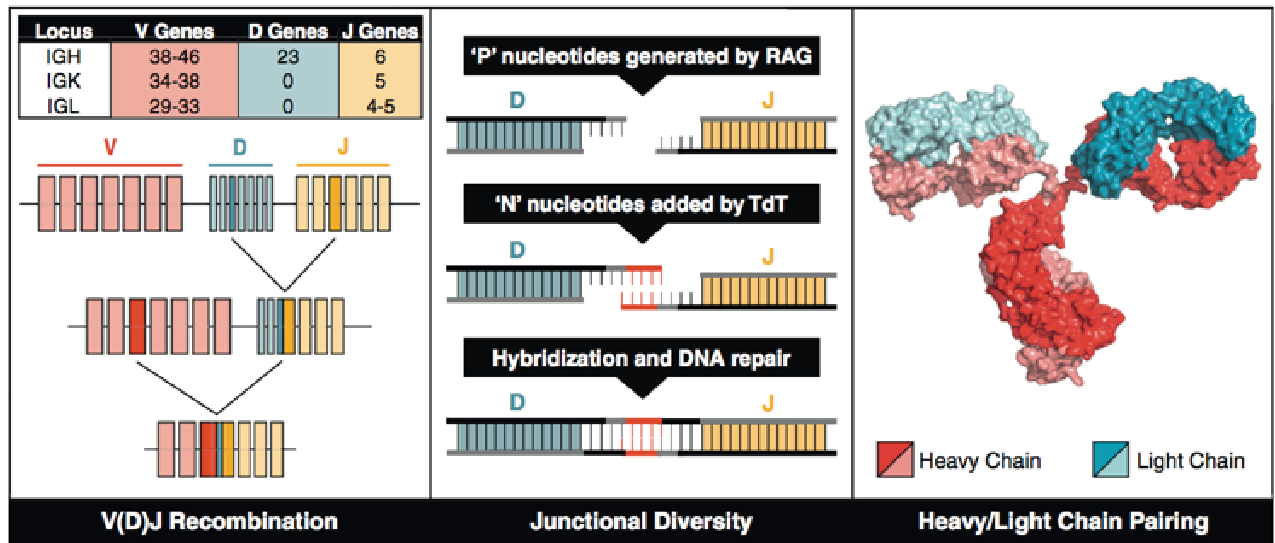
\includegraphics[width=1\textwidth]{images/intro/figure1_2.pdf}
\caption[Overview of Antibody Recombination]{
Overview of Antibody Recombination. Diversity in the antigen-combining site of the B-cell receptor repertoire (and thus also in the corresponding secreted antibody repertoire) is mediated by three principal molecular mechanisms, illustrated in the three panels, left, middle, and right. Figure adapted from \citep{Finn:2013fr}.
}
\label{fig:Diversification}
\end{figure}


\subsubsection{Somatic Hypermutation to Enable Diversity}
Maturation of the antibody repertoire to hone specificity is known as somatic hypermutation (SHM) and is initiated by the somatic hypermutation machinery (SHAM). Somatic hypermutation is the response to antigen stimulus and happens in various lymph tissues. This process is known as the secondary diversification \citep{Tonegawa:1983vw,Brenner:1966vj}. 

Na�ve, antigen inexperienced B-cells undergo the SHM process upon recognition of an infectious agent. It is through the SHM process, which occurs primarily in lymphoid tissue, mutate the variable region of their antibody genes (figure \ref{fig:somaticdiversification})  \citep{Li:2004it,MacLennan:1992we}. Many of these mutations have no effect on antigen recognition and many have deleterious effects on either antigen recognition or proper folding of the antibody protein. However, some mutations produce antibodies with improved affinity for the target pathogenic epitope  \citep{Casali:2006dn}.Thus, the SHM process provides a basis for the positive selection of high affinity antibodies that are characteristic of a mature immune response  \citep{MacLennan:1994bo}. SHM introduces point mutations at a frequency of approximately 103 mutations per base pair, which is 106-fold higher than the rate of spontaneous mutation in other genes \citep{Rajewsky:1987wn}. Activation-induced cytidine deaminase (AID) is required for SHM and initiates the SHM process by the deamination of cytosine nucleotides, which results in the conversion of cytosine to uracil \citep{Muramatsu:2000um,Muramatsu:1999ur}. Deamination thus produces a uracil-guanine mismatch, and several possible processes result in the error-prone repair of the mismatch. The precise mechanism(s) responsible for error-prone repair during SHM are not known, although several DNA repair mechanisms have been shown to be critical to the SHM process, including base excision repair and mismatch repair \citep{Phung:1998vx,Rada:1998tf,Wiesendanger:2000wl,DiNoia:2002ix,Zheng:2005dy}. 

\begin{figure}%Somatic Diversification
\centering
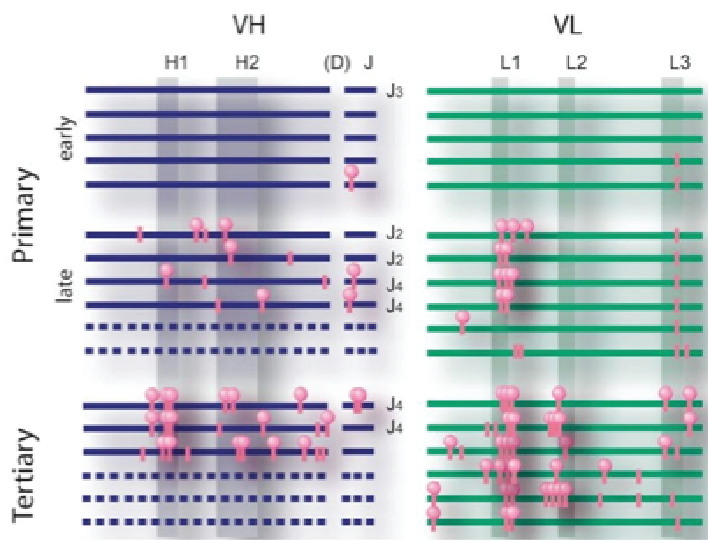
\includegraphics[width=.5\textwidth]{images/intro/figure1_3.pdf}
\caption[Somatic Mutations in Response to Antigen Stimulus]{
Somatic mutations in response to antigen stimulus. The VH gene and VL gene are shown for various VH and VL pairs represented by blue and green lines. The CDR loops H1-H3 and L1-L3 are darkened. The pink dots represent mutations. The early response has little to no somatic mutations recapitulating na�ve repertoire. The late and response starts developing mutations. A second challenge with the same antigen shows even more mutations to hone specificity. Figure adapted from \citep{Berek:1988ww}, redrawn by C., Scotti }
\label{fig:somaticdiversification}
\end{figure}

\subsubsection{Implications for Antibody Structure}
Antibody complementarity determining regions (CDRs, also referred to as hypervariable regions, figure /ref{fig:abwithloops}) are the primary region of antigen recognition that lie at the apical tip of the antibody structure (figure \ref{fig:abwithloops}). They are preferentially targeted for affinity maturation by the SHM machinery, making them the most variable regions of the antibody gene \citep{Padlan:1994wq}.  Structurally, the CDRs are largely loop-based, which make them sufficiently flexible to incorporate the substitutions and without compromising structural integrity. Framework regions (FRs) are highly structured and less able to accommodate somatic mutations \citep{Jimenez:2003by}.

\begin{figure}%Antibody with Loops
\centering
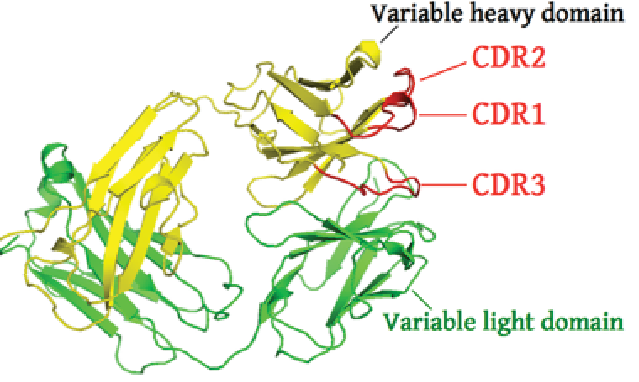
\includegraphics[width=.5\textwidth]{images/intro/figure1_4.pdf}
\caption[Antibody Structure with CDR Loops]{Antibody structure with CDRs.The light chain in green with the LCDRs not pictured. The heavy chain is shown in yellow with the HCDRs shown in red. Figure adapted from PDB: 1IGT\citep{Harris:1997eo}.
}
\label{fig:abwithloops}
\end{figure}

\section{HIV Pandemic Overview}
HIV-1 is an unprecedented health problem that continues to remain a worldwide pandemic. Since the recognition of acquired immune deficiency syndrome (AIDS) in 1981 \citep{Gottlieb:1981ge} followed by the discovery of it's causative agent, human immunodeficiency virus (HIV) in 1983 \citep{BarreSinoussi:1983ta}, an estimated 65 million have been infected with over 25 million deaths \citep{Hemelaar:2012cv}. The amount of people estimated to be still living with HIV is 30 million, many of which live in the developing world \citep{Anonymous:1vVbBZBX}.

More than 40 different nonhuman primate species harbor SIV infections, with each species carrying a species-specific virus. Each independent zoonotic transmission can generate a different lineage. HIV type 1 (HIV-1), thought to be transmitted from chimpanzees in the Congo around 1900 \citep{Keele:2006fi}, is the most common and further is split into groups M, N, O, and P. HIV-1 group M is responsible for the global pandemic and is further split into subtypes clades A-D,F-H, J and K that are tropic to specific regions. Within each subtype variation of the amino acids vary as much as 30\%. For example, clade B is the most common in North America while clade C is the most common in Sub-Saharan Africa (figure \ref{fig:pandemic}). If a full genome sequence is found that are recombinations of different HIV-1 group M subtypes, they are designated circulating recombinant forms (CRFs) if they are epidemiologically linked or unique recombinant forms if they are unlinked (URF) \citep{Robertson:2000bv}.

A major contributing factor to HIV spread and defense is its potential for enormous genetic diversity. This genetic diversity stems from the error rates of the reverse-transcription machinery which lacks proof-reading capabilities \citep{Ho:1995fn}. This genetic diversity gives rise to sequence divergence of up to 10\% within a single individual \citep{Korber:2001tc}. This is one of the many defense mechanisms HIV uses to evade host response and contemporary vaccination strategies.

\begin{figure}%HIV Pandemic
\centering
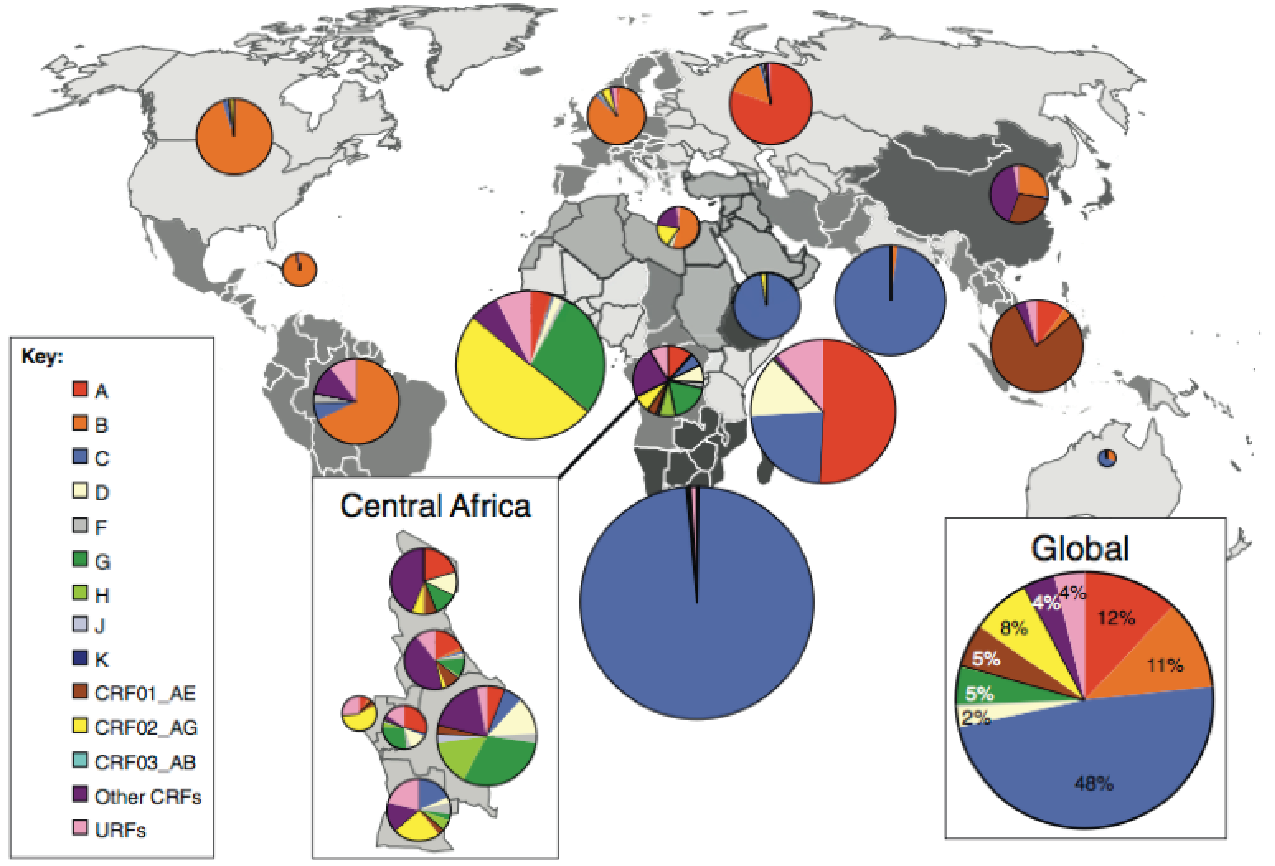
\includegraphics[width=1\textwidth]{images/intro/figure1_5.pdf}
\caption[Global Distributions of HIV-1 Subtypes]{Global distributions of HIV-1 subtypes. In the main figure, pie charts representing the distribution of HIV-1 subtypes and recombinants from 2004 to 2007, colored by HIV-1 subtype. Adapted from UNAIDS report 2013.}.
\label{fig:pandemic}
\end{figure}

\subsection{The HIV Virus Genome and Structure}
HIV-1 is an enveloped virus containing a duplicate positive-strand RNA genome (figure \ref{fig:hivgenome}, left panel). The functional spike on the surface of the virion is the Env glycoprotein and is coded by the env gene (figure \ref{fig:hivgenome}, right panel). The Env glycoprotein complex is originally produced as a single-chain glycoprotein precursor, gp160, which is cleaved by a cellular protease. Cleavage of gp160 results in the cell-surface attachment protein gp120 and the membrane-spanning protein gp41. The gp160 cleavage products are noncovalently linked and assemble into a trimer of gp120-gp41 heterodimers that are expressed on the virion surface \citep{Kowalski:1987vq}. Gp120 is heavily glycosylated, with nearly half the total mass being the result of N-linked glycans \citep{Poignard:2001hu}. It is composed of five variable regions (V1-V5) interspersed with five constant regions (C1-C5) \citep{Starcich:1986ty}. The principle function of the glycoprotein spike is to facilitate cell entry by binding to the primary cell-surface receptor, CD4, and one of the two co-receptors, CCR5 and CXCR4. Binding to the receptor and co-receptor is accomplished by gp120, and fusion of the viral and cell membranes is mediated by gp41 \citep{Zwick:2001ei}. 

The rest of the genome is composed of viral enzymes such as the error-prone reverse transcriptase, the integrase that allows integration of viral DNA to the host genome, and protease, to allow cleavage of gene products into their functional subunits. There are also structural proteins that lie below the envelope that make up the inner matrix and nucleocapsid. There are also several accessory proteins, Vpu, Vif, Vpr, P6, Nef, Rev, and Tat which aid in combating host defense or enhancing viral fitness \citep{Fields:2007vu}. All of these proteins serve a significant purpose to the virulence and life cycle of the HIV-1 virus but will not be discussed further and they have low antigenicity to antibodies, the primary focus of my research. A list of their genes and gene products can be found in figure \ref{fig:hivgenome}, right panel. 

\begin{figure}%HIV Genome and Structure
\centering
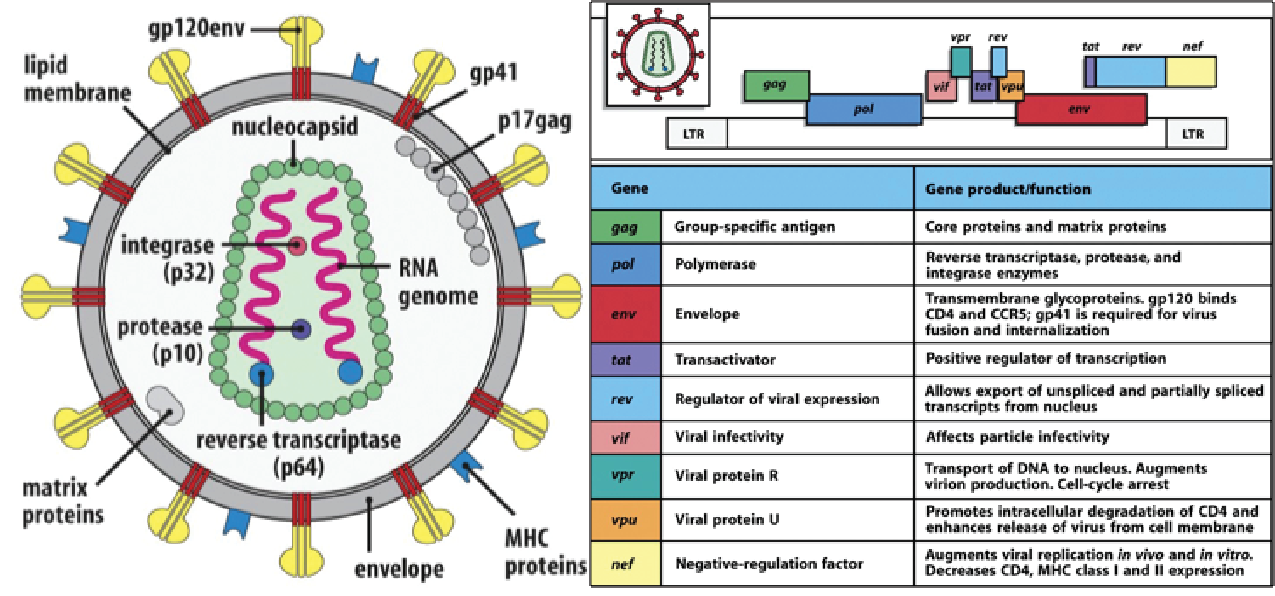
\includegraphics[width=1\textwidth]{images/intro/figure1_6.pdf}
\caption[Simplified View of HIV Structure and Genome]{Simplified view of HIV structure and genome. The proteins that make up the virus structure are displayed as a schematic. The virus is coded by a duplicated RNA genome (pink) surrounding by a viral nucleocapsid proteins. The inner envelope is supported by gag protein with gp120 envelope shown as a trimer bound to gp41. These trimeric "spikes" are responsible for infectivity by binding CD4-binding sites (left panel).\linebreak Each gene is represented in a different color and localizes to either the nucleocapsid (green) or the outer envelope (red). }
\label{fig:hivgenome}
\end{figure}

\subsection{The Viral Spike and Humoral Resistance}
The failure of conventional vaccines to prime the immune system for a broad response against HIV-1 challenge is partially explained thorough the structural definition of the HIV-1 spike reveling mechanisms of defense. Much of the surface is covered in carbohydrates that shield neutralizing epitopes \citep{Binley:2010du}. The conserved CD4 binding site is recessed and sits behind the hypervariable loops \citep{Burton:2005db}. The co-receptor binding site is also recessed unless CD4 has triggered a conformational shift exposing this region \citep{Harris:2011gm}. Another defense is the relative lability of the trimeric complex \citep{Wyatt:1998vs}. The gp120 head often sheds creating "stumps" that serve as decoy epitopes against the viral complex \citep{Liu:2008in}. In addition there are few functional trimeric spikes on the surface of HIV limiting immune response to few locations on the virion. 

The biggest defense is sequence variability. Much of the antibody response is targeted to the hypervariable loops that can easily change sequence without much consequence to viral fitness. This is why the humoral response produces autologous or strain-specific neutralizers that must catch up to a constantly evolving antigenic target \citep{Albert:1990ua,Gray:2007hi,Pilgrim:1997wj,Richman:2003dc,Sagar:2006eb,Wei:2003ea}.  

\section{Broadly Neutralizing Antibodies to HIV}
Given the major defenses of the HIV envelope structure, it provided a rather discouraging view for vaccine development. In fact, only four modestly neutralizing antibodies were discovered between the 1991 and 2010 \citep{Burton:2005db,Kwong:2012cc}, two membrane proximal extracellular region (MPER) binders 2F5 and 4E10 \citep{Zwick:2001ei,Muster:1994tw}, a CD4 binding site neutralizer b12 \citep{Burton:1994wl}, a complex carbohydrate binder 2G12 \citep{Trkola:1996vb} (table \ref{tab:allmabs}, figure \ref{fig:bnabmap}). 

It was thought that the conventional vaccine strategies could not stimulate immune system to produce broadly neutralizing antibodies to HIV do to the extreme variability of the viruses and the capability of the virus to escape an antibody response. Then, high throughput neutralization assays were developed that could rapidly test sera for neutralization capacity \textit{in vitro} allowing researchers to accurately quantify the neutralizing response of HIV infected patients \citep{Binley:2004hd,Blish:2007ef,Li:2005go,Mascola:2005fe,Montefiori:2005jt}. Several groups found that there were multiple patients that could neutralize very genetically diverse panels HIV variants, even those that were not in that patients sub-type \citep{Binley:2008gj,DoriaRose:2010js,Simek:2009cn,Wu:2006cd}. That lead to longitudinal studies to show how long it took for a broadly neutralizing response to develop. Researchers showed that this generally took anywhere from 2-4 years \citep{Gray:2011ki,Mikell:2011hr,Moore:2011hy} with earliest time points arising at 1 year \citep{DoriaRose:2014ic}. The question still remained if those neutralizing responses were caused by few monoclonal antibody responses or just a large polyclonal response \citep{Gray:2007hi,Binley:2008gj,Li:2007em,Rong:2009ky,Sather:2009jb,Scheid:2009bv,Tomaras:2011bc,Walker:2010bm}.

The question was answered by the recent explosion of new broadly neutralizing antibodies isolated by multiple research groups \citep{Corti:2013ex}. It started with two new isolates, PG9 and PG16, from an African donor that lead to the discovery of a completely new neutralizing epitope which is the focus of my research (figure  \ref{fig:bnabmap}) \citep{Walker:2009cd}. Both PG9 and PG16 bind to a proteoglycan epitope through an extended HCDR3 structure \citep{McLellan:2011dg}. 

The discovery of PG9 and PG16 lead to newly characterized antibodies using similar techniques such as microneutralization screening, high-throughput sequencing, and hybridoma technology. The Haynes laboratory characterized additional long HCDR3 antibodies that bound similarly as PG9 and PG16 but with less breadth \citep{Bonsignori:2011dq}. There are other classes of glycan dependent antibodies isolated by the Poignard group that bind the V3 and beta-strands that are higher potency than PG9 and PG16 \citep{Walker:2011ew}. Other MPER antibodies have also been characterized to by the Connors group such as 1E08 that neutralizes 98\% of viruses \citep{Huang:2012fh}. Focused epitopes designed computationally can also be used to identity some of the most potent antibodies to date (the VRC series) \citep{Wu:2010jv}. These antibodies were identified using a designed scaffold of gp120 that 'knocked-out' non-neutralizing epitopes. Thus, only neutralizing antibodies would be isolated upon binding. I will not enumerate further on all the antibodies characterized to date, their method of isolation and if any longitudinal studies were used to determine their pathways of development. These characteristics are summed in table \ref{tab:allmabs} and figure \ref{fig:bnabmap}.

It is interesting to note, and important for the work that will be presented here, that the broadly neutralizing antibodies to date share one of two characteristics. They are either highly somatically mutated, indicative of years of chronic infection and selective pressure, or have a very long non-canonical HCDR3 (figure \ref{fig:bnabcorrelabion}). Both of these characteristics make it difficult to elicit in a vaccine attempt, but will be discussed further in the upcoming chapters.

%comes from excel to table
% Table generated by Excel2LaTeX from sheet 'page 1'
\begin{sidewaystable}[htbp]
  \centering
\begin{tabular}{lllllcl}
\toprule
Antibody & Specificity & Breadth & V$_{H}$ & SHM & HCDR3 Length & Screening Strategy \\ 
\midrule
	2F5 & gp41 MPER & \textasciitilde60-70\% & 2-5 & 15.2 & 24 & gp160 and p24 binding \\
	4E10 & gp41 MPER & \textasciitilde96-98\% & 1-69 & 15.6 & 20 & gp160 and p24 binding   \\ 
	1EO8 & gp41 MPER & \textasciitilde98\% & 3-15 & 22.1 & 22 & Microneutralization  \\ 
	2G12 & gp120 glycans & \textasciitilde25-30\% & 3-21 & 33.6 & 16 & gp160 and p24 binding   \\ 
	PGT128 & Glycans and V3 $\beta$-strand & \textasciitilde70-75\% & 4-39 & 27.9 & 21 & Microneutralization  \\ 
	PGT127 & Glycans and V3 $\beta$-strand & \textasciitilde50\% & 4-39 & 23.2 & 21 & Microneutralization   \\ 
	PGT121 & Complex type V3 N-glycans & \textasciitilde65-70\% & 4-59 & 21.2 & 26 & Microneutralization  \\ 
	10-1074 & Complex type V3 N-glycans & \textasciitilde55-60\% & 4-59 & 24.4 & 26 & gp140 binding   \\ 
	PGT135 & Glycans and V4 & \textasciitilde30-35\% & 4-39 & 26.8 & 20 & Microneutralization   \\ 
	PG9/PG16 & Glycans and V1/V2 & \textasciitilde75-80\% & 3-33 & 15.4-16.8 & 30 & Microneutralization   \\ 
	CH01- CH04 & Glycans and V1/V2 & \textasciitilde50\% & 3-20 & 23.3-19.5 & 26 & Microneutralization  \\
	PGT145 & Glycans and V1/V2 & \textasciitilde75-80\% & 1-8 & 22.8 & 33 & Microneutralization \\
	b12 & gp120 CD4bs & \textasciitilde30-35\% & 1-3 & 17.3 & 20 & Phage library  \\ 
	HJ16 & gp120 CD4bs & \textasciitilde30-35\% & 3-30 & 36.7 & 21 & EBV- immortalization  \\ 
	VRC01 & gp120 CD4bs & \textasciitilde90-95\% & 1-2 & 38.7 & 14 & Cell sorting/RT-PCR \\
	VRC03 & gp120 CD4bs & \textasciitilde50\% & 1-2 & 34.9 & 16 & Cell sorting/RT-PCR \\ 
	3BNC117 & gp120 CD4bs & \textasciitilde85-90\% & 1-2 & 36.9 & 12 & Cell sorting/RT-PCR  \\ 
	3BNC60 & gp120 CD4bs & NA & 1-2 & 36.9 & 12 & Cell sorting/RT-PCR \\
	NIH45-46 & gp120 CD4bs & \textasciitilde90\% & 1-2 & 44 & 18 & Cell sorting/RT-PCR \\
	CH30- CH34 & gp120 CD4bs & \textasciitilde80\% & 1-2 & 31.9-31.9 & 15 & Cell sorting/RT-PCR  \\
	PGV04 & gp120 CD4bs & \textasciitilde85-90\% & 1-2 & 38.2 & 16 & Cell sorting/RT-PCR\\
	3BC176 & CD4i/V3 & \textasciitilde60-70\% & 1-2 & 29.4 & 19 & Cell sorting/RT-PCR \\
\bottomrule
\end{tabular}
\caption[Broadly Neutralizing Antibody Properties]{Broadly neutralizing antibody properties. Breadth refers to the amount of viruses tested that fall below 50 $\mu$g/mL.  V$_{H}$ is the heavy chain accessed from IMGT, SHM is the somatic hypermutation percentage of heavy chains as assessed from IMGT. Table adapted from (2013)\citep{Corti:2013ex}. }
\label{tab:allmabs}%
\end{sidewaystable}%


\begin{figure}%HIV man map
\centering
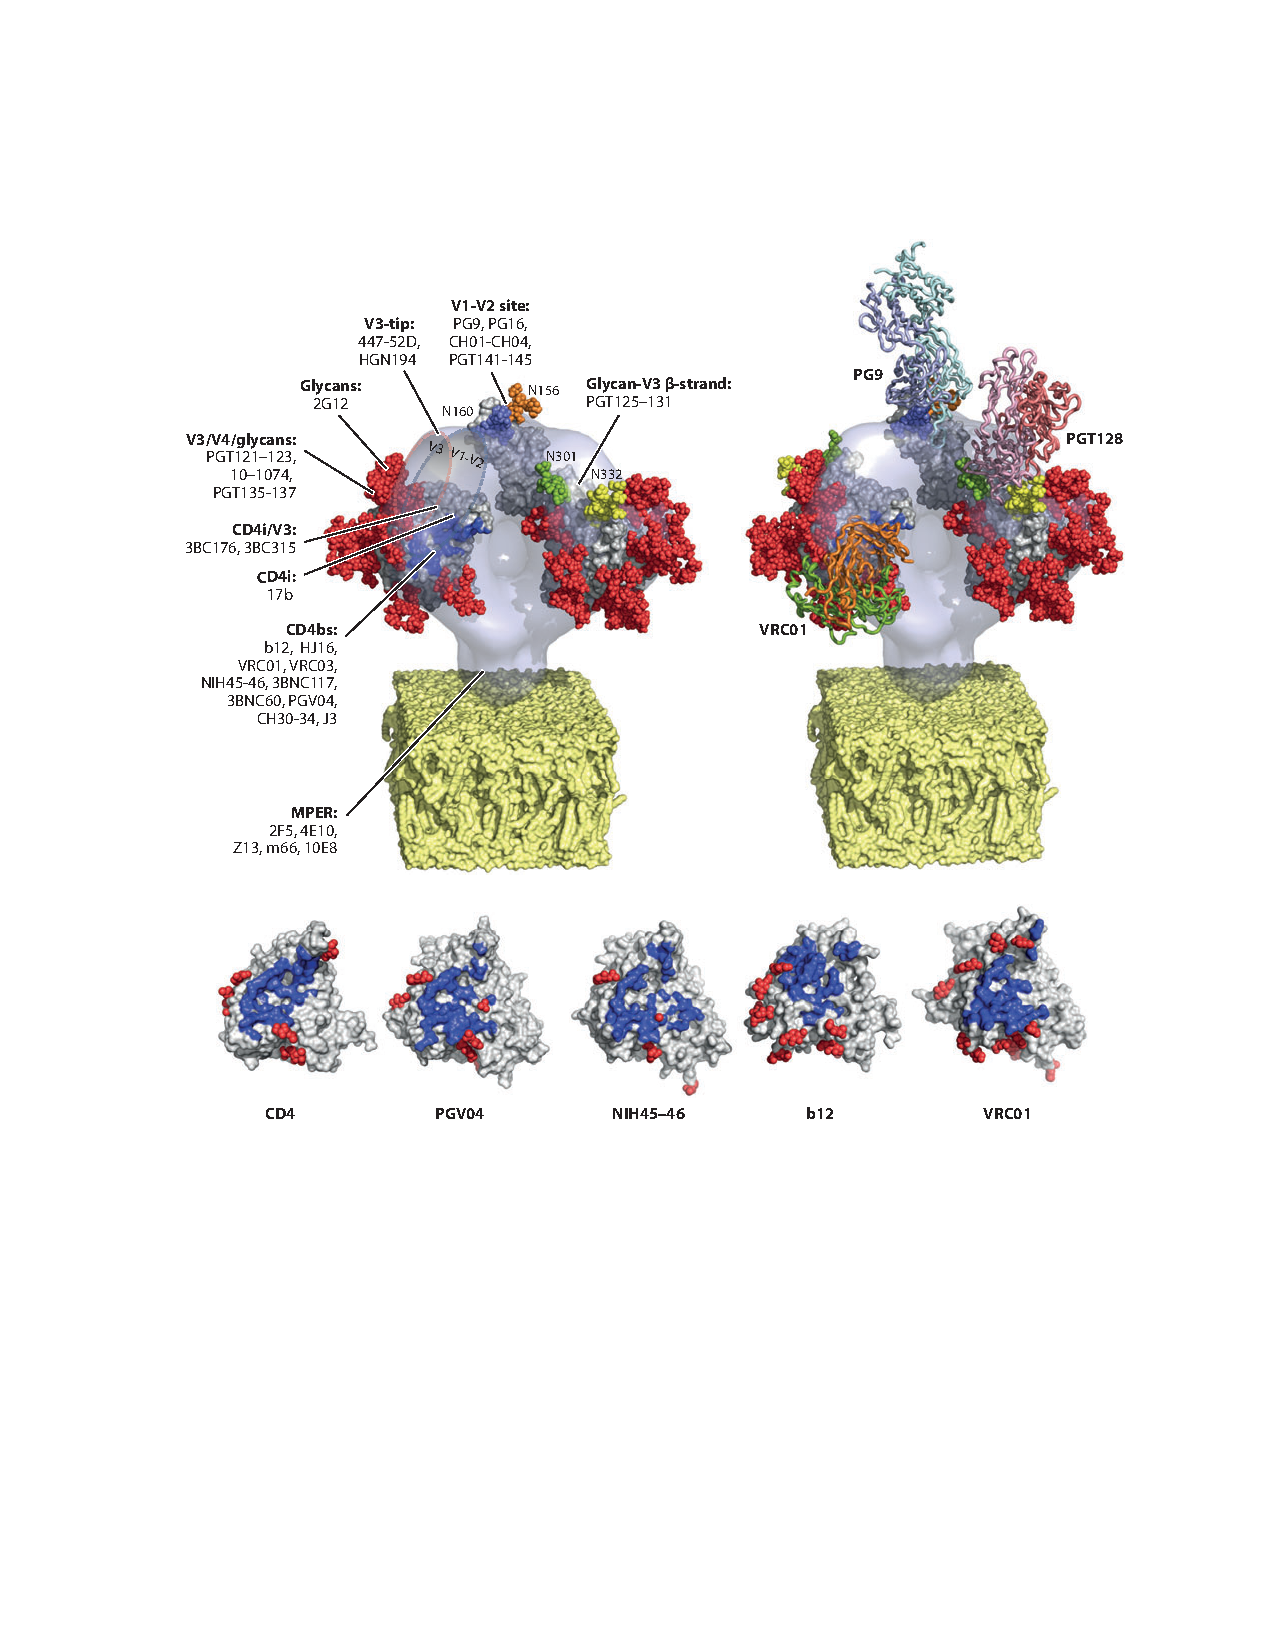
\includegraphics[width=1\textwidth]{images/intro/figure1_7.pdf}
\caption[Broadly Neutralizing Epitopes Mapped to HIV Env Trimer]{Model of the HIV-1 Env trimeric glycoprotein bound to broadly neutralizing antibodies. The left panel shows the major sites targeted by broadly neutralizing antibodies. The approximate positioning of the V1/V2 and V3 loops is shown, and the CD4 footprint on the gp120 monomer is highlighted in blue. The right panel shows the FABs of broadly neutralizing antibodies VRC01 (3NGB), PG9 (3US2), and PGT128 (3TYG) bound to gp120. Carbohydrates (oligomannose, red spheres) were modeled on the unliganded YU2 gp120 core (3TGQ) using GlyProt, with the exception of the glycans bound by PGT128 and PG9 (depicted with different colors), which were taken from the structures. The location of PG9 above the trimeric gp120 is approximate; VRC01 and PGT128 FABS were docked by superposition with the unliganded YU2 gp120 model. The bottom panel shows in blue the footprints of CD4 (1GC1) and the CD4bs-specific antibodies PGV04 (3SE9), NIH45-46 (3U7Y), b12 (3DNL), and VRC01 (3NGB). Figure adapted from \citep{Corti:2013ex}}
\label{fig:bnabmap}
\end{figure}

\begin{figure}%HIV man map
\centering
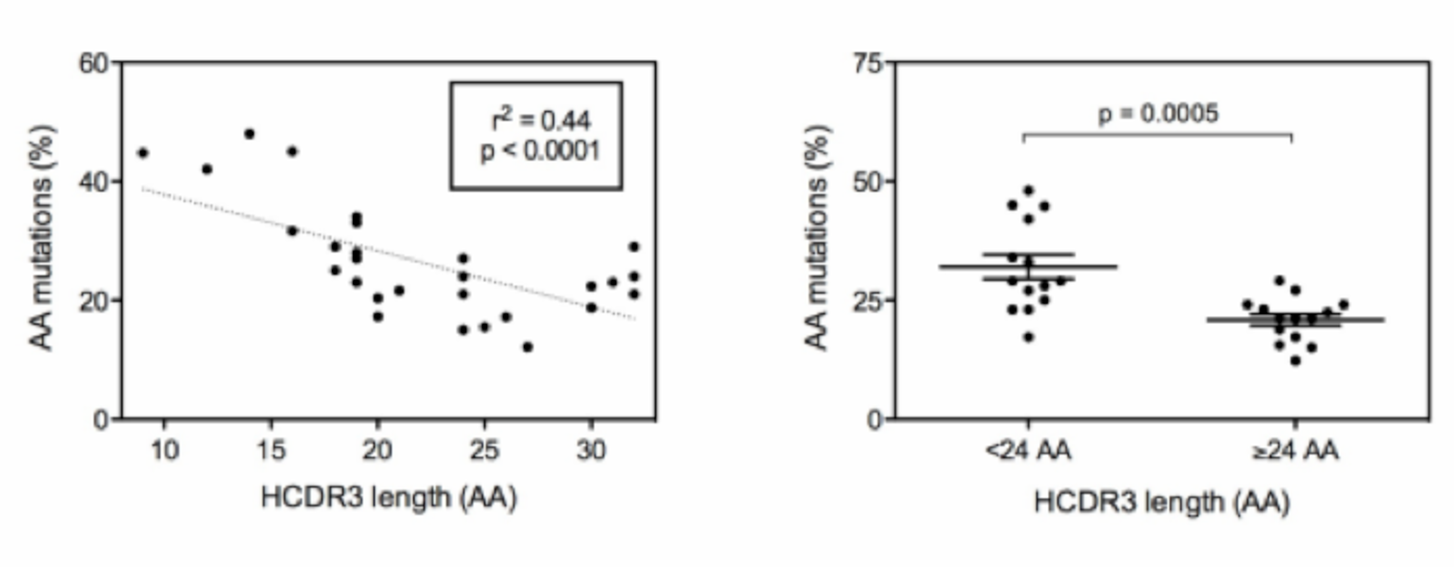
\includegraphics[width=1\textwidth]{images/intro/figure1_8.pdf}
\caption[Trends of HIV bNAbs]{Trends of HIV bNAbs. Plotted on the y-axis is the frequency of amino acid mutations of the currently characterized bNAbs. On the x-axis is the length of the heavy chain CDR3 (HCDR3). A negative correlation exists between the frequency of mutations and the HCDR3 length (r$^{2}$ = 0.44, left panel). When long HCDR3s (>24 AA) are binned against canonical length HCDR3s (<24AA), there is a statistical significance between the frequencies of amino acid mutation (p = 0.0005, right panel).}
\label{fig:bnabcorrelation}
\end{figure}



\section{Rosetta}
Many software packages exist for the specific task of threading, minimization, and design. The Rosetta software suite includes algorithms for all of these tasks and was developed for computational modeling and analysis of protein structures; further, it is free for noncommercial users. It has enabled notable scientific advances in computational biology, including de novo protein design, enzyme design, ligand docking and structure prediction of biological macromolecules and macromolecular complexes \citep{Rohl:2004bl,Siegel:2010bc,Kuhlman:2003kp,Davis:2009bf,Misura:2006hs,Davis:2009fx,Das:2008gf}. The broad spectrum of applications available through Rosetta allows for multiple computational problems to be addressed in one software framework. To aid in the understanding of Rosetta-specific language, a supplementary glossary has been provided in the appendix section for the Rosetta glossary.
One of the most common applications of Rosetta is protein structure prediction via \textit{de novo} folding and comparative modeling \citep{Kaufmann:2010ea,Rohl:2004bl}. \textit{De novo} folding can be used to predict the protein's tertiary structure when only the primary sequence of a protein is known. However, to date, Rosetta has been shown to successfully fold only small, soluble proteins (fewer than 150 amino acids), and it performs best if the proteins are mainly composed of secondary structural elements \citep{Meiler:2003dt}. Structures of helical membrane proteins between 51 and 145 residues were predicted to within 4� of the native structure \citep{YarovYarovoy:2006br}, but only very small proteins (up to 80 residues) have been predicted to atomic-detail accuracy \citep{Bradley:2005bu,Bradley:2005fs,Das:2007em}. Accurate prediction of larger and/or more complex proteins can be achieved with the addition of experimental data, such as NMR chemical shifts and distance data \citep{Rohl:2005kx,Lange:2012hp,Lange:2012wo}.

Another application, protein threading, refers to the tolerance of a tertiary fold given PDB coordinates. The Rosetta scoring function evaluates how well a sequence can "tolerate" a structure. It is often known as the "inverse folding problem". The known template structure of which a sequence will be threaded reduces almost all-conformational space by providing a protein backbone scaffold. Threading has played a major role in aiding experimental design and the interpretation of experimental results. They can be used to help predict structure-function relationships \citep{Kaufmann:2009cq}, and aiding in designing proteins for binding pathogens \citep{Azoitei:2011jd,Correia:2010ck,Correia:2011bk,Correia:2011hr,Schief:2009ke}, determining thermostable proteins \citep{Stranges:2013em,Kuhlman:2002ka,Der:2011gt},and aid in the determination of target residues for site-directed mutagenesis \citep{Keeble:2008hd,Fortenberry:2011gx}. 

\subsection{The Rosetta Energy Function}
All of the applications described above rely on a metric to score predictive models. This metric in Rosetta is referred to as the Rosetta energy function. The scoring function in Rosetta is derived empirically through analysis of observed geometries of a subset of proteins in the PDB. We call this scoring function a knowledge-based scoring function, since it relies on previous knowledge of observed structures. The measurements include, but are not limited to, radius of gyration, packing density, distance/angle between hydrogen bonds and distance between two polar atoms. The measurements are converted into an energy function through Bayesian statistics \citep{Simons:1997do,Metropolis:1953vj}.

The scoring function in Rosetta can be separated into two main categories: centroid-based scoring and all-atom scoring. The former is used for de novo folding and initial rounds of loop building \citep{Rohl:2005kx,Simons:1997do,Simons:1999wp}. The side chains are represented as "super-atoms", or "centroids", which limit the degrees of freedom to be sampled while preserving some of the chemical and physical properties of the side chain. Although this centroid-based scoring function is important for de novo folding, the folding protocol is not covered within the scope of this article.

The all-atom scoring function represents side chains in atomic detail. Similarly to the centroid-based scoring function, the all-atom scoring function comprises weighted individual terms that are summed to create a total energy for a protein. Most of the scoring terms are derived from knowledge-based potentials. The scoring function contains Newtonian physics based terms, including a 6-12 Lennard-Jones potential and a solvation potential. The 6-12 Lennard-Jones potential is split into two terms, an attractive term (fa\_atr) and a repulsive term (fa\_rep), for all van der Waals interactions \citep{Kuhlman:2000tc,Neria:1996wj}. The solvation potential (fa\_sol) models water implicitly and penalizes the burial of polar atoms \citep{Lazaridis:1999wi}. Interatomic electrostatic interactions are captured through a pair potential (fa\_pair) \citep{Simons:1999wp}, and an orientation-dependent hydrogen bond potential for long-range and short-range hydrogen bonding (hbond\_sc, hbond\_lr\_bb, hbond\_sr\_bb, and hbond\_bb\_sc, respectively) \citep{Gordon:1999tk,Wedemeyer:2003kh}. In addition to the electrostatic terms, the Rosetta all-atom scoring function contains terms that dictate side chain conformations according to the Dunbrack rotamer library (fa\_dun) \citep{Dunbrack:1993jt,Dunbrack:1997kh}, preference for a specific amino acid given a pair of phi/psi angles (p\_aa\_pp), and preference for the phi/psi angles in a Ramachandran plot (rama) \citep{Rohl:2004bl,Wedemeyer:2003kh,RAMACHANDRAN:1963wj}.

\subsection{Rosetta Minimization}
\label{subsec:Rosetta Minimization}
When new sequences are threaded, or rebuilt onto target protein structures, it is often necessary to go through a round of energetic minimization. The protein undergoes refinement using the Rosetta all-atom scoring function to yield an all-atom protein model \citep{Bradley:2005bu}. Both threading and docking in Rosetta involve an all-atom refinement of the protein. The protocol used for structural refinement, visually described in figure \ref{fig:minimization}, is often referred to as "relax". The goal of the relax protocol is to explore the local conformational space and to energetically minimize the protein. During this process, local interactions are improved by iterative side-chain repacking, in which new side chain conformations, or "rotamers", are selected from the Dunbrack library \citep{Dunbrack:1993jt}; and by gradient-based minimization of the entire model, in which the energy of the model is minimized as a function of the score. These small structural changes are evaluated according to the all-atom scoring function and are sampled in a Metropolis Monte Carlo method \citep{Metropolis:1953vj}. The relax protocol has been shown to markedly lower the overall energy of the Rosetta model and is essential to achieving atomic detail accuracy \citep{Das:2008gf,Bradley:2005fs,Rohl:2005kx}.

\begin{figure}%minimization
\centering
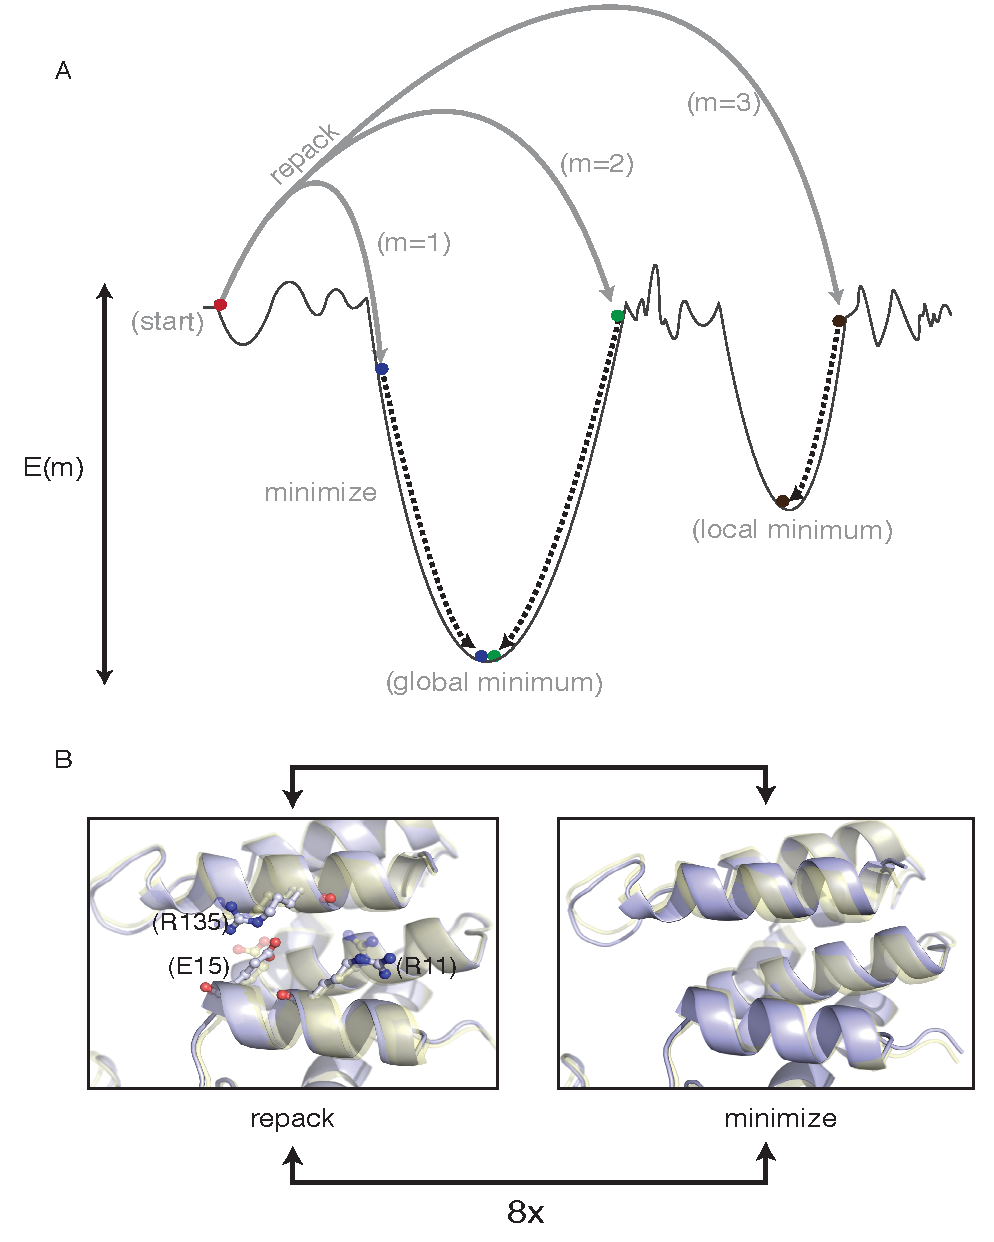
\includegraphics[scale=.7]{images/intro/figure1_9.pdf}
\caption[Refinement via Relax]{Refinement via Relax. Simplified energy landscape of a protein structure. The relax protocol combines small backbone perturbations with side-chain repacking. The coupling of Monte Carlo sampling with the Metropolis selection criterion allows for sampling of diverse conformations on the energy landscape. The final step is a gradient-based minimization of all torsion angles to move the model into the closest local energy minimum (A). Comparison of structural perturbations introduced by the repack and minimization steps. During repacking, the backbone of the input models fixed, whereas side-chain conformations from the rotamer library33 are sampled. Comparison of the initial (transparent yellow) and final (light blue) models reveals conservation of the R135 rotamer but changes to the R11 and E15 rotamers. Minimization affects all angles and changes the backbone conformation (B).}
\label{fig:minimization}
\end{figure}



\subsection{Rosetta Design}
Protein design, seeks to determine an amino acid sequence that folds into a given protein structure or performs a given function. The RosettaDesign algorithm is an iterative process that energetically optimizes both the structure and sequence of a protein \citep{Kuhlman:2003kp}. RosettaDesign alternates between rounds of fixed backbone sequence optimization and flexible backbone energy minimization. During the sequence optimization step, a Monte Carlo simulated annealing search is used to sample the sequence space. Every amino acid is considered at each position in the sequence, and rotamers are picked from to the Dunbrack library \citep{Dunbrack:1993jt}. After each round of Monte Carlo sequence optimization, the backbone is relaxed to accommodate the designed amino acids. The practical uses of RosettaDesign can be divided into five basic categories: design of novel folds. Redesign of existing proteins, design to enhance knowledge of structure, enzyme design, and design applied to translational medicine. 

\subsubsection{Design of Novel Folds}
The RosettaDesign method was implemented by Kuhlman and colleagues \citep{Kuhlman:2000tc}. The method has been used for the \textit{de novo} design of a fold that was not (yet) represented in the PDB \citep{Kuhlman:2003kp}. This was arguably the start of the "golden age" of protein design and gave credibility to the algorithm. A starting backbone model consisting of a five-strand $\beta$-sheet and two packed helices was constructed with the Rosetta \textit{de novo} protocol using distance constraints derived from a two-dimensional sketch. The sequence was iteratively designed with five simulation trials of 15 cycles each. The final sequence was expressed, and the structure was determined using X-ray crystallography. The experimental structure has a deviation to the predicted structure of <1.1 angstroms.

\subsubsection{Redesign of Existing Proteins}
When nine globular proteins were stripped of all side chains and then redesigned using RosettaDesign, the average sequence recovery was 35\% for all residues \citep{Dantas:2003vt}. In four of nine cases, the protein stability improved as measured by chemical denaturation. The structure of a redesigned human protein was determined experimentally.  RosettaDesign was then used to systematically identify mutations of carboxypeptidase that would improve the stability of the protein. All of the tested mutants were more stable than the wild-type protein, with the top-scoring mutant having a reduction of free energy of 5.2 kcal/mol.

\subsubsection{Design to Enhance Knowledge of Structure}
Protein design approaches have enhanced our knowledge of how protein sequence relates to protein structure. For instance, the finding that designed protein sequences are highly similar to the native sequence suggests that native protein sequences are optimal for their structure \citep{Kuhlman:2000tc}. Babor and Kortemme investigated the antibody sequence-structure relationship using RosettaDesign. They demonstrated that native sequences of antibody HCDR3 loops are optimal for conformational flexibility \citep{Babor:2009it}. The authors collected pairs of unbound and antigen-bound antibody structures. They used multiconstraint design to find low-scoring sequences that were consistent with both unbound and bound structures. The sequences predicted by multiconstraint design were more similar to the native sequences than the sequences predicted to preferentially bind either the unbound or bound conformations. 

\subsubsection{Enzyme Design}
The RosettaMatch algorithm starts from the protein backbone and attempts to build toward the specified transition state geometry \citep{Zanghellini:2006is}. In this method, all possible active site positions are defined for the protein scaffold, and rotamers from the Dunbrack library are placed at each sequence position in the catalytic site. The sequence of the area surrounding the catalytic site is then designed. 
Recently, the RosettaMatch algorithm was used to design enzymes that catalyze the retro-aldol reaction \citep{Jiang:2008jk}.The degrees of freedom in the transition state, the orientation of the active site side chains, and the conformations of the active site side chains were simultaneously optimized. Of 72 models tested, a total of 32 were found to have catalytic activity as much as four orders of magnitude greater than that of an uncatalyzed reaction. Two of the active enzymes were crystallized. The experimental structures share a high degree of similarity with the computational design although the loop regions surrounding the catalytic site show significant variance from the model.

Computationally designed functional Kemp elimination catalysts using RosettaMatch have also been designed. Quantum chemical predictions were used to generate an idealized transition state model, and RosettaMatch was used to search for backbone configurations that would support the predicted transition sate \citep{Rothlisberger:2008ef}. 

\subsubsection{Design Applied to Translational Medicine}
The successes of the RosettaDesign algorithm in predicting new sequences that optimize binding and answer questions about protein structure lead to its application to more bio-medical applications such as vaccine design and protein therapeutics. Fleishman et al. used the paratope of an antibody to find hotspot positions that neutralized influenza. Using these positions, they designed a protein that would properly present a mimic of the paratope. The crystal structure of the design indicated that it did indeed present mimicry while functional studies confirmed its neutralization capacity \citep{Fleishman:2011fx}.
The works of the Schief group have expanded design to explore novel scaffolding approaches to be used as immunogens. Using RosettaDesign, they presented the epitope to broadly neutralizing antibodies 2F5 and 4E10 to HIV which elicited this class of antibody in animal models \citep{Correia:2010ck,Ofek:2010bv}. In addition, they have used RosettaDesign to target potently neutralizing antibodies against the CD4 site while eliminated binding to non-neutralizing antibodies that bind to decoy epitopes \citep{Wu:2010jv}. More recently, this lab has used design to mimic an epitope to RSV that is now being tried in animal models \citep{Correia:2014jp}.

A current major challenge in protein design is the \textit{de novo} design of a novel protein-protein interface. So far, the most successful attempts at \textit{de novo} interface design have been relatively modest, focusing on small proteins and yielding micromolar affinity \citep{Mandell:2009he,Huang:2007ge}. This small boost affinity often requires display technology to increase potency and specificity. The Rosetta community is well aware of these limitations and work on increasing the accuracy of predicted interface mutations, particularly around hydrogen bonding networks and explicit solvent models \citep{Combs:2012tl}. 



%\include{introduction}
%\chapter{Design of Native-Like Proteins through an Exposure-Dependent Environment Potential}
\label{chap:nv_kbp}
\section{Introduction}
\subsection{Computational design of proteins is an active area of research}
The design of protein surfaces with proper amino acid composition is critical to preventing aggregation and allowing for correct protein folding \citep{Chandler:2005ds}.
Thermostabilization of enzymes and design of proteins with novel folds are two possible applications of the present research. 

\subsection{The current Rosetta solvation model does not penalize the burial of apolar atoms}
As there are relatively few explicit interactions of amino acids on the protein surface, the total energy of a residue is dominated by Rosetta's implicit solvation model.
The solvation model currently used by Rosetta is a function developed by Lazaridis and Karplus \citep{Lazaridis:1999wi}.
This potential estimates the solvation free energy of an atom from a reference free energy, where the atom is essentially fully solvent-exposed.
For every nearby atom, a cost of "desolvation" is added in a pairwise decomposable and distance-dependent manner.
This procedure aligns with the protein folding process, where amino acids move from a completely exposed location into varying degrees of burial.
While the model is parameterized for all amino acid atom types, it is driven by high desolvation penalties of polar atoms.
For this reason, it is quite insensitive to the burial of apolar atoms because desolvation energies are small. 

\subsection{RosettaDesign currently has difficulty designing protein surfaces}
This paradigm of desolvation is useful for determining energy changes in the folding of a monomeric protein.
However, hydrophobic patches on the surface of a \textit{de novo} designed protein are hardly penalized, as the environment of these amino acids did not change in the folding process.
At present, RosettaDesign excels in the design of tightly packed protein cores, while the protein surface is often poorly composed and requires manual adjustment \citep{Dantas:2003vt}.
We hypothesize that native proteins have evolved to minimize unspecific aggregation, a fact that is ignored by the desolvation potential.
Evolutionary pressures exerted on protein sequence composition by the requirement of protein solubility are difficult to model with a typical physics-based model, but can be modeled effectively with a knowledge-based energy potential. 

\subsection{Description of the RosettaDesign energy function}
The RosettaDesign energy function is a weighted composite of the Lazaridis-Karplus solvation free energy potential, attractive and repulsive interactions, an action center pairwise potential to approximate electrostatic interactions, an orientation-dependent hydrogen bonding potential \citep{Kortemme:2003td}, and reference energies for amino acid type and conformation \citep{Dantas:2003vt}. 
Amino acid reference energies and scoring function weights are optimized to maximize sequence recovery in a protein design benchmark.
Reference energies can be viewed as the ground state energy of an amino acid in an essentially fully exposed, unfolded peptide chain.
Hence, these reference energies can disfavor apolar amino acids on the surface, thereby representing some of the evolutionary pressure to prevent aggregation.
However, the same reference energies are also fitted to reflect amino acid propensities in nature independently of burial.
In addition, the reference energies are fitted to maximize sequence recovery and thereby counterweight other inaccuracies in the RosettaDesign energy function.
As a result, the reference energies form a container term that combines multiple effects that can be difficult to disentangle, and it provides a corrective power against exposed hydrophobic amino acids on the surface.

\subsection{A knowledge based environment potential was developed to improve the quality of protein surface designs}
To improve upon the above shortcomings of RosettaDesign, we implemented the \acf{NV}-based \ac{KBP} previously described by Durham et al. \citep{Durham:2009kt}.
This neighbor vector environment \ac{KBP} converts the likelihood to see an amino acid at a given level of exposure into an environment energy.
The \ac{NV} environment \ac{KBP} encapsulates both desolvation energy and evolutionary biases against apolar amino acids at the protein surface with amino acid level resolution.

\subsection{The development of a more accurate approximation of \acs{SASA} }
The usefulness of an environment potential based on burial is contingent on an accurate measure of burial.
\ac{SASA} is the most accurate means of calculating amino acid burial but is generally time-consuming to compute, limiting its usefulness in protein design.
RosettaDesign currently uses a \ac{NCR} for estimating solvent accessibility in the pair potential.
While the \ac{NCR} method correlates with residue burial, high inaccuracies are common in surface and partially exposed positions (Figure \ref{fig:nv_ncr_comparison}). 

\begin{figure}
\centering
\includegraphics[width=4in]{figures/nv_kbp/nv_ncr_comparison}
\caption{
Comparison of \acs{NV} and \acs{NCR} measures to \acs{rSASA}.
In both panels, a color map plots the difference between a surface approximation method and the normalized \acs{rSASA} value.
A residue for which the \acs{SASA} approximation matches \acs{rSASA} exactly would have a score of 0.0 and be colored white.
Regions of the surface in red are categorized as more solvent exposed than by \acs{rSASA}, while regions in blue are categorized as less solvent exposed than by \acs{rSASA}.
(A) protein 7DFR colored by the \acs{NCR} approximation of surface accessibility as used in Rosetta.
(B) protein 7DFR colored using the \acs{NV} approximation.
The \acs{NV} measure has significantly smaller deviations from the \acs{rSASA} standard with a mean of 0.14 compared to the mean deviation of 0.20 seen with the \acs{NCR} measure.
Additionally, the \acs{NV} measure is more consistent, with a standard deviation of 0.11 compared to the standard deviation of 0.46 seen with the \acs{NCR} metric.
Panels A and B illustrate the improvement in consistency, as areas of score deviation in Panel B are smaller and generally less "patchy" in their appearance.
}
\label{fig:nv_ncr_comparison}
\end{figure}

\subsubsection{The \acs{NV} \acs{SASA} approximation was previously developed by Durham et al.}
To overcome the limitations of the \ac{NCR} burial approximation, an \ac{NV} approximation of residue burial was implemented.
For a schematic representation of the \ac{NV} algorithm, see Figure \ref{fig:nv_schematic}.
The \ac{NV} algorithm and \ac{KBP} generated and described by Durham et al \citep{Durham:2009kt}
was used in our implementation.
Proteins selected for deriving the \ac{KBP} were monomeric, globular proteins, which do not engage in obligate, and therefore strong, protein-protein interactions.
It is expected that some of these proteins will engage in transient interactions with other proteins, however, these interactions will be weaker.
As a result, the noise added to the \ac{KBP} by these interactions will be of low magnitude and uniform.

\begin{figure}
\centering
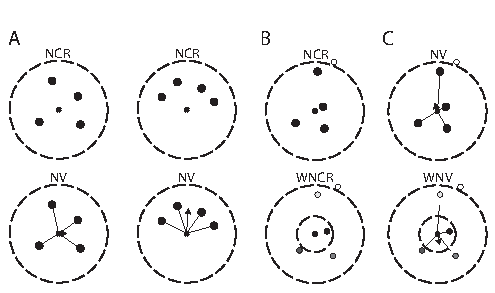
\includegraphics[width=4in]{figures/nv_kbp/nv_schematic}
\caption{
(A) The left and right panels both have the same Rosetta neighbor count \citep{Dantas:2003vt} but very different degrees of burial.
The neighbor vector method is able to distinguish between these cases by calculating the vectors between the query residue and its neighbors.
The length of the vector indicates the degree of burial, with shorter vectors representing more buried residues. 
(B) The \acf{WNCR} method gives a higher weight to neighbors near the query residue, smoothing the effect of small changes in composition on the measured degree of burial. 
(C) The combination of the \acs{NV} and \acs{WNCR} methods results in a more accurate measure of residue distribution. 
In all panels, dotted lines represent lower and upper bounds for counts, the X marks the query residue, and circles represent residues surrounding the query residue.
}
\label{fig:nv_schematic}
\end{figure}

\subsubsection{\acs{NV} is a more accurate approximation of \acs{SASA} than other methods} 
The half sphere approximation method developed by Hamelryck in 2005 \citep{Hamelryck:2005kt} approximates surface accessibility by counting the number of residues in a half sphere below the side chain of each amino acid.
The half sphere count is directly related to residue burial.
\ac{HSE} is implemented in the freely available BioPython library, and this library was used to compare performance of \ac{HSE} and \ac{NV} to \ac{rSASA} (calculated using NACCESS).
The per residue exposure was calculated for each of the proteins in the 42 protein benchmark set, and adjusted $R^{2}$ values were calculated for the correlation of each measure to \ac{rSASA}.
The adjusted correlation factor $R^{2}$ value for \ac{HSE} to \ac{rSASA} was 0.68, while the adjusted correlation factor $R^{2}$ for the \ac{NV} method was 0.86.
This suggests that while \ac{HSE} is conceptually simpler, it does not perform as accurately as \ac{NV} for proteins in our benchmark set.

\subsubsection{Mapping \acs{NV} results to \acs{rSASA} results} 
A linear regression modeling the correlation between \ac{rSASA} values (in the range of 0 to 1 calculated using NACCESS) and \ac{NV} score (range 0 to 1) was generated based on all proteins in the 42 protein benchmark set.
The equation for the resulting linear regression model was $rSASA = 1.29(NV)-0.11$ and had an $R^{2}$ of 0.86.
Based on this model, residues with \ac{NV} scores between 0.00 to 0.24 will have an approximate \ac{rSASA} value of 0.0 to 0.19, residues with \ac{NV} scores from 0.25 to 0.39 will have an approximate \ac{rSASA} value of 0.21 to 0.39, and residues with \ac{NV} scores between 0.40 to 1.00 will have an approximate \ac{rSASA} value of 0.40 to 1.10.

\subsection{Overview of RosettaLigand scoring term architecture}
Terms in the RosettaDesign energy function can take the form of either single-body or two-body terms.
Two-body terms describe energies that pertain to the interaction between residues, such as the energy associated with hydrogen bonding, while single-body terms describe energies that pertain only to a single residue.
The resulting \ac{NV} environment \ac{KBP} was implemented as a single-body term in the RosettaDesign energy function.
RosettaDesign revision 39040 was used in all calculations.  

\subsection{Sequence recovery is insufficient as a metric for assessing protein design}
Computationally assessing the performance of a protein design algorithm is inherently challenging.
Historically, percent sequence recovery has been used as a metric for the quality of a protein design, as it has been observed that protein sequences are frequently close to optimal for a given fold \citep{Kuhlman:2000tc}.
However, many protein folds having large variations in sequence are frequently seen in nature \citep{Chothia:1986tm}.
Of the 74,608 protein chains present in the \ac{SCOP} database as of 2009, only 1,280 individual folds are observed \citep{Schaeffer:2011fe}.
In many positions, particularly on the surface of proteins, multiple residues can be tolerated with similar energies.
This finding limits sequence recovery as a measure for successful protein design because the design of a different but tolerated amino acid is counted as a failure.
To resolve this problem, we introduce a metric based on sequence homology. A \ac{PSSM} is derived from a \ac{BLAST} query of the native sequence of a protein.
The percent recovery of amino acids with positive values in the \ac{PSSM} determines recovery of evolutionarily tolerated amino acids. 

\section{Experimental Procedures}

\subsection{Optimization of the weight of the new energy term}
The RosettaDesign energy function is a linear combination of individual energy terms.
As a result, the addition of a new energy term will impact the energy function as a whole.
To address this, each energy term is multiplied by a weight, and these weights must be carefully optimized following the introduction of a new term.
In most cases, it is not necessary to optimize the entire scoring function when a new term is added.
Instead, only the terms that describe similar information as the new term are optimized.
In the case of the \ac{NV} environment \ac{KBP}, the solvation free energy potential and the reference energies must also be optimized. 

\subsubsection{Development of a training data set}
To ensure that the optimized weights would apply to a wide range of proteins, a set of 100 soluble protein crystal structures from the \ac{PDB} were used in optimization.
Structures were selected to have a sequence homology of less than 25\%, a length of 67-179 amino acids, and a resolution better than 2.0 \AA.
The optimization was conducted using a five-way cross validation protocol.
In this protocol, the 100 crystal structures described above were split into 5 groups of 20 structures each.
In each component of the five-way validation, 80 proteins were used during optimization, and the remaining 20 were used to benchmark the resulting weights.
In statistics generated from the benchmarking phase of the optimization process, results from all 5 sets of 20 proteins are combined, resulting in a total benchmark set of 100 proteins. 

\subsubsection{Particle Swarm Optimization scheme}
An iterative particle swarm approach \citep{Chen:2007ua} was used to optimize the weights.
The RosettaDesign standard energy function was used as an initial point for optimization, and the weight of the \ac{NV} environment \ac{KBP} was arbitrarily given an initial weight of 1.0.
Twenty rounds of particle swarm optimization were performed for each component of the five-way cross validation described above.
The weights were optimized to maximize the \ac{PSSM} score of proteins designed using the energy function (Table \ref{table:energy_weights}).
The \ac{PSSM} for each protein was generated from a PSI-PRED \ac{BLAST} query of the protein structure sequence using an \textit{e} threshold of 0.001 and 3 iterations.
The \ac{NR} sequence database was used.
The average sequence identity between the query sequence and all other sequences in the generated \ac{PSSM}s was 30\% for both benchmark sets.

\begin{table}
\scriptsize
\renewcommand{\tabcolsep}{0.09cm}
\centering
%This was supplement T1

\begin{tabular}{|r|r|r|r|r|r|r|r|r|r|}
\hline
& & & \multicolumn{5}{c|}{Five way cross validation sets} & &  \\
\hline
& Rosetta Scoring term & Scoring term description & 1 & 2 & 3 & 4 & 5 & Mean & Standard Deviation \\
\hline
\multirow{2}{*}{Free Weights} & fa\_sol & Solvation Free Energy Potential & 0.558 & 0.569 & 0.563 & 0.547 & 0.585 & 0.564 & 0.014 \\
\cline{2-10}
& neigh\_vect & NV environment KBP & 1.025 & 1.013 & 0.996 & 1.059 & 0.978 & 1.014 & 0.030 \\
\hline
\multirow{17}{*}{Fixed Weights} & fa\_atr & Attractive force & \multicolumn{5}{c|}{0.8} & 0.8 & 0.0\\
\cline{2-10}
& fa\_rep & Repulsive force & \multicolumn{5}{c|}{0.44} & 0.44 & 0.0\\
\cline{2-10}
& fa\_intra\_rep & Intra-residue repulsive force & \multicolumn{5}{c|}{0.004} & 0.004 & 0.0\\
\cline{2-10}
& pro\_close & Proline closure bonus & \multicolumn{5}{c|}{1.0} & 1.0 & 0.0\\
\cline{2-10}
& fa\_pair & Pair energy & \multicolumn{5}{c|}{0.49} & 0.49 & 0.0\\
\cline{2-10}
& hbond\_sr\_bb & Hydrogen bonding: short range backbone & \multicolumn{5}{c|}{0.585} & 0.585 & 0.0\\
\cline{2-10}
& hbond\_lr\_bb & Hydrogen bonding: long range backbone & \multicolumn{5}{c|}{1.17} & 1.17 & 0.0\\
\cline{2-10}
& hbond\_bb\_sc & Hydrogren bonding: backbone-sidechain & \multicolumn{5}{c|}{1.17} & 1.17 & 0.0\\
\cline{2-10}
& hbond\_sc & Hydrogen bonding: sidechain-sidechain & \multicolumn{5}{c|}{1.1} & 1.1 & 0.0 \\
\cline{2-10}
& dslf\_ss\_dst & Disulfide sidechain distance & \multicolumn{5}{c|}{1} & 1 & 0.0\\
\cline{2-10}
& dslf\_cs\_ang & Disulfide cystine sulfur angle & \multicolumn{5}{c|}{1} & 1 & 0.0\\
\cline{2-10}
& dslf\_ss\_dih & Disulfide sidechain-sidechain dihederal & \multicolumn{5}{c|}{1} & 1 & 0.0\\
\cline{2-10}
& dslf\_ca\_dih & Disulfide C?-sidechain dihederal & \multicolumn{5}{c|}{1} & 1 & 0.0\\
\cline{2-10}
& rama & Ramachandran score & \multicolumn{5}{c|}{0.2} & 0.2 & 0.0\\
\cline{2-10}
& omega & Omega angle score & \multicolumn{5}{c|}{0.5} & 0.5 & 0.0\\
\cline{2-10}
& p\_aa\_pp & Probability of an AA given phi/psi angle & \multicolumn{5}{c|}{0.32} & 0.32 & 0.0 \\
\cline{2-10}
& fa\_dun & dunbrack rotamer library & \multicolumn{5}{c|}{0.56} & 0.56 & 0.0\\
\hline
\end{tabular}
\caption{A table showing the individual weights included in the optimization, and their values in each of the five cross validation sets.  The mean and standard deviation of each free weight is also shown. }
\label{table:energy_weights}
\end{table}

\subsubsection{Reference energies were optimized in addition to the \acs{NV} environment \acs{KBP} term}
Because the standard deviation of the averaged reference averaged reference energies was relatively high, the reference energies of the averaged energy function are optimized to reduce the overall sequence composition biases introduced during design (Table \ref{table:ref_energy_weights}).

\subsubsection{Two separate optimization experiments were performed}
In the first experiment, the reference energies, solvation free energy potential, and the \ac{NV} environment \ac{KBP} were optimized.
In the second experiment, the \ac{NV} environment \ac{KBP} was excluded from the energy function, and only the reference energies were optimized.
This second experiment acts as a control and makes it possible to distinguish between design improvements due to reference energy optimization and design improvements due to the addition of the \ac{NV} environment \ac{KBP} itself.
While both \ac{NV} environment \ac{KBP} and the solvation free energy potential describe overlapping but different phenomena at different levels of resolution: The \ac{NV} environment \ac{KBP} is an indirect measure of solvation free energy and evolutionary biases against aggregation.
This energy term functions at amino acid resolution and will be independent of side chain conformation.
In contrast, the solvation free energy potential is at atomic resolution incorporating a specific model of solvation.
While the solvation free energy potential does an inadequate job of accounting for biases against aggregation on the protein surface, it is highly accurate in avoiding burial of polar atoms, and is important to determine side chain conformation.

\begin{table}
\scriptsize
\renewcommand{\tabcolsep}{0.09cm}
\centering
%This was supplement T2
\begin{tabular}{|c|r|r|r|r|r|r|r|r|}
\hline
 \textbf{AA name} & \multicolumn{5}{c|}{\textbf{Five way cross validation sets}} & & &  \\
\hline
 & \textbf{1} & \textbf{2} & \textbf{3} & \textbf{4} & \textbf{5} & \textbf{Mean} & \textbf{Standard Deviation} & \textbf{Re-optimized Energies} \\
\hline
\hline
A & -0.313519 & -0.345577 & -0.332996 & -0.299376 & -0.311145 & -0.3205226 & 0.018489708 & -0.280778\\
\hline
C & -0.186065 & -0.267899 & -0.251004 & -0.203121 & -0.273443 & -0.2363064 & 0.039429392 & -0.191836\\
\hline
D & -0.0516543 & -0.152027 & -0.117976 & -0.04581 & -0.158867 & -0.10526686 & 0.053922242 & -0.0894836\\
\hline
E & -0.116794 & -0.225243 & -0.221177 & -0.13447 & -0.230275 & -0.1855918 & 0.055185343 & -0.163316\\
\hline
F & 0.979346 & 1.00881 & 1.09867 & 0.976394 & 1.03573 & 1.01979 & 0.05028824 & 1.0029\\
\hline
G & 0.187346 & 0.862973 & 0.681024 & 0.322192 & 0.952133 & 0.6011336 & 0.334354423 & 0.318222\\
\hline
H & 0.773425 & 0.727736 & 0.727848 & 0.755789 & 0.683065 & 0.7335726 & 0.034276949 & 0.738805\\
\hline
I & -0.0879415 & -0.063614 & -0.0662562 & -0.147069 & -0.0349584 & -0.07996782 & 0.041974551 & -0.0892347\\
\hline
K & -0.0356543 & -0.113405 & -0.125976 & -0.0465226 & -0.104256 & -0.08516278 & 0.041146221 & -0.0565743\\
\hline
L & -0.288888 & -0.27654 & -0.302976 & -0.350292 & -0.286631 & -0.3010654 & 0.029090569 & -0.295543\\
\hline
M & -0.475654 & -0.472027 & -0.532784 & -0.514173 & -0.478867 & -0.494701 & 0.027189556 & -0.488778\\
\hline
N & -0.523683 & -0.559673 & -0.549976 & -0.500635 & -0.582867 & -0.5433668 & 0.031950345 & -0.532584\\
\hline
P & -0.486622 & -0.556899 & -0.579705 & -0.488828 & -0.551983 & -0.5328074 & 0.042469908 & -0.494263\\
\hline
Q & -0.481516 & -0.58252 & -0.554953 & -0.491584 & -0.569756 & -0.5360658 & 0.046379036 & -0.497717\\
\hline
R & -0.280894 & -0.364054 & -0.324666 & -0.255467 & -0.389405 & -0.3228972 & 0.055748092 & -0.294276\\
\hline
S & -0.396296 & -0.436734 & -0.438423 & -0.37399 & -0.437601 & -0.4166088 & 0.029793151 & -0.393299\\
\hline
T & -0.312536 & -0.375408 & -0.373141 & -0.307255 & -0.368256 & -0.3473192 & 0.034311466 & -0.332279\\
\hline
V & -0.175465 & -0.166283 & -0.166976 & -0.217204 & -0.134509 & -0.1720874 & 0.029660029 & -0.176609\\
\hline
W & 1.43079 & 1.50528 & 1.52902 & 1.46971 & 1.42618 & 1.472196 & 0.045170863 & 1.47413\\
\hline
Y & 0.842276 & 0.853102 & 0.902422 & 0.851712 & 0.81571 & 0.8530444 & 0.031423486 & 0.842514\\
\hline

\end{tabular}

\caption{A table showing the optimized weights of the reference energies for each amino acid. }
\label{table:ref_energy_weights}
\end{table}

\subsection{Analysis of the optimization experiments}
The optimization experiments described above produce five individual energy functions, each generated from one section of the five-way cross validation.
To produce a single optimized scoring function for general use, the weights from the five optimized energy functions are averaged together, and the reference energies of the averaged energy function are optimized using the set of 100 proteins used in the initial  cross validation.
The averaged energy function is benchmarked on an independent set of 42 protein crystal structures, in which the proteins have a sequence homology of less than 15\%, a size range of 150-225, and a resolution less than 1.5 \AA.
Note that these proteins are larger and more complex than the proteins used in the more time-consuming weight optimization procedure.
As a result, this benchmark poses a formidable challenge for the RosettaDesign fixed backbone design algorithm.
Several different metrics were used during benchmarking to assess the quality of designed proteins.
Percent \ac{PSSM} recovery was the primary benchmarking metric used in the study.
Percent \ac{PSSM} recovery was calculated as the percentage of residues that were designed as residues with a positive score in the \ac{PSSM} of the native protein.
In addition, the percent sequence recovery was measured as the percentage of residues that remained in as the native residue after design. 

\subsubsection{Percent \acs{PSSM} recovery calculation}
\label{subsubsec:percent_pssm_calc}
The percent \ac{PSSM} recovery per residue, percent sequence recovery per residue, and the change in overall sequence composition were also calculated for each designed protein.
Percent \ac{PSSM} recovery per residue is calculated as $\frac{num\ pssm\ recovered}{num\ designed}$ where $num\ pssm\ recovered$ is the number of residues with a given identity which were designed to a residue with a positive \ac{PSSM} score, and $num\ designed$ is the total number of residues designed. 
Percent sequence recovery per residue was calculated as $\frac{num\ recovered}{num\ designed}$ where $num\ recovered$ is the number of residues with a given identity which were designed to an identical residue.
In addition to calculating overall percent sequence recovery, sequence recovery by chemical group was also calculated.
In this metric, residues were grouped into the categories polar (Ser, Thr, Asn, Gln), non-polar (Ala, Val, Leu, Met, Ile), aromatic (Phe, Tyr, Trp), charged (Lys, Arg, His, Asp, Glu), and other (Cys, Pro, Gly). 
A residue was counted as recovered if it was mutated to another residue within the same group.

\subsubsection{Percent sequence recovery calculation}
Percent sequence composition change per amino acid type was calculated as $\frac{d-n}{num\ designed}$ where $d$ is the count of designed residues of a given type, and $n$ is the count of native residues.
To compute the change in overall sequence composition, a \ac{RMS} method was used.
\ac{RMS} percent sequence composition change was calculated as shown in equation \ref{eqn:rms}, where $statistical\ metric$ is one of the metrics described in section \ref{subsubsec:percent_pssm_calc} (shown as black bars in figures \ref{fig:overall_crossval_changes} and \ref{fig:overall_independent_changes}).

\begin{equation}
\label{eqn:rms}
RMS=\sqrt{\frac{1}{20}\sum^{20}_{i=1..20}(statistical\ metric)^{2}}
\end{equation}

\subsubsection{Calculation of metrics by degree of burial}
All of the above metrics were calculated for the entire protein, as well as the deeply buried region, surface region, and a boundary layer between the two.
For this study, the buried region is defined as all residues with a \ac{NV} score between 0.00 and 0.24, the boundary is defined as 0.25 to 0.39, and the surface region is defined as 0.40 to 1.00.
The performance of the optimized energy functions via these benchmarks was compared to the performance of the standard RosettaDesign energy function.

The benchmarks described above are intended as a measure of how well RosettaDesign is accomplishing its goal of generating low-energy, native-like protein sequences.
In a well-optimized energy function, we expect that the percent \ac{PSSM} recovery will increase compared to the standard RosettaDesign energy function.
We also expect that the percent sequence recovery will remain similar to that obtained with the standard energy function.
Finally, we expect that a well-optimized energy function will exhibit smaller biases in sequence composition compared to proteins designed with the standard energy function.

\section{Results}

The percent \ac{PSSM} recovery and percent sequence recovery calculated for the 100 proteins used in the five-way cross validation are shown in Table \ref{table:burial_100}.
The results of \ac{PSSM} recovery and sequence recovery analysis show that the optimized \ac{NV} environment \ac{KBP} energy function exhibits a 5.2\% improvement in percent \ac{PSSM} recovery compared to the standard energy function and that 3.6\% of this improvement was a result of reference energy optimization.
The \ac{NV} environment \ac{KBP} energy function showed a 1.6\% improvement in percent sequence recovery compared to the standard RosettaDesign energy function and a 2.4\% improvement if only reference energies are optimized.  

\begin{table}
\scriptsize
\renewcommand{\tabcolsep}{0.09cm}
\centering
\begin{tabular}{|r||r|r|r|r|r|r|}
\hline
 & \multicolumn{3}{c}{\textbf{Percent PSSM Recovery}} & \multicolumn{3}{|c|}{\textbf{Percent Sequence Recovery}}\\
\hline
  & \textbf{Standard} & \textbf{Reference} & \textbf{NV environment KBP} & \textbf{Standard} & \textbf{Reference} & \textbf{NV environment KBP}\\
\hline
\hline
Buried & 73.4\% & 77.1\% & 78.9\% & 64.9\% & 66.5\% & 65.5\% \\
\hline
Boundary & 72.1\% & 75.3\% & 77.3\% & 44.3\% & 46.6\% & 45.5\% \\
\hline
Surface & 70.4\% & 74.4\% & 75.9\% & 32.8\% & 35.9\% & 35.5\% \\
\hline
Overall & 72.0\% & 75.6\% & 77.2\% & 45.7\% & 48.1\% & 47.3\% \\
\hline
\end{tabular}
\caption{Percent \acs{PSSM} recovery and percent sequence recovery by degree of burial for 100 proteins used in optimization. "Standard" refers to the standard energy function, "Reference" refers to the modified standard energy function in which the reference energies were re-optimized, and "\acs{NV} environment \acs{KBP}" refers to the optimized energy function incorporating the \acs{NV} environment energy term.}
\label{table:burial_100}
\end{table}

\subsection{The \ac{NV} environment \ac{KBP} improves PSSM recovery and reduces sequence composition bias}
The percent change in composition between native and designed sequences for the 100 proteins used in the five-fold cross-validation is shown in Figure \ref{fig:overall_crossval_changes}A.
Proteins designed with the \ac{NV} environment \ac{KBP} energy function show a decrease in the average magnitude of sequence composition biases introduced during design compared to proteins designed with the standard energy function.
Proteins designed with the standard energy function exhibit an \ac{RMS} percent change in sequence composition of 2.0\%, while proteins designed with the \ac{NV} environment \ac{KBP} show an \ac{RMS} percent change in sequence composition of 1.0\%.
Figure \ref{fig:overall_crossval_changes}B shows that \ac{RMS} per residue \ac{PSSM} recovery increased from 3.8\% with the standard energy function to 4.2\% with the \ac{NV} environment \ac{KBP}, and \ref{fig:overall_crossval_changes}C shows that \ac{RMS} per residue sequence recovery remained relatively constant between the standard energy function and \ac{NV} environment \ac{KBP}. 

\begin{figure}
\centering
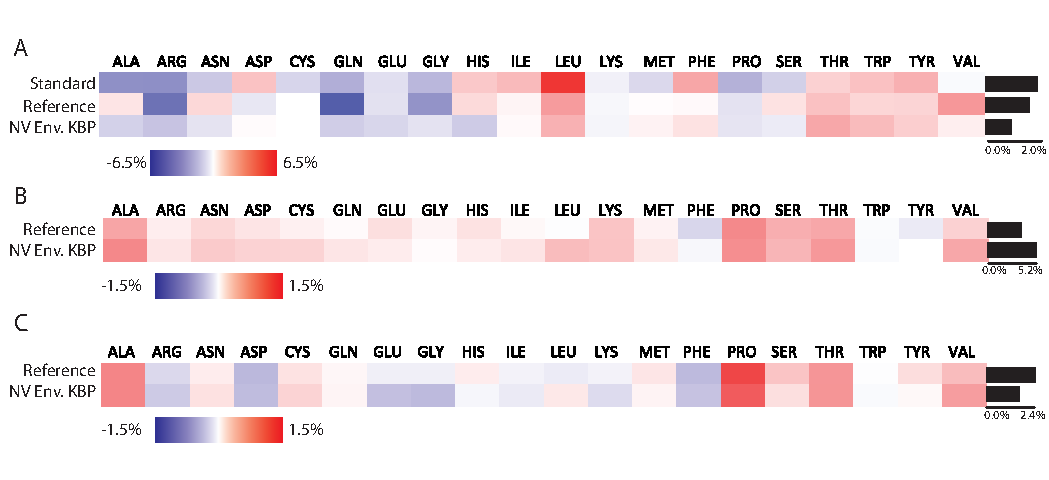
\includegraphics[width=4in]{figures/nv_kbp/overall_crossval_changes}
\caption{
A) shows the percent change in overall sequence composition between native and designed proteins for all 100 structures in the five-way cross-validation set.
The black bars show the \acs{RMS} percent composition change.
B) shows the percent \acs{PSSM} recovery for all 100 structures in the five-way cross-validation set.  The black bars show \acs{RMS} percent \acs{PSSM} recovery.
C) percent sequence recovery for all 100 structures in the five-way cross-validation set.  The black bars show \acs{RMS} percent sequence recovery.	
}
\label{fig:overall_crossval_changes}
\end{figure}

\subsection{Independent benchmarking of a single averaged energy function shows improved performance}
The energy functions produced with the five-way validation were averaged to produce a single energy function, the reference energies of this averaged function were optimized, and the benchmarking analysis used above was repeated using the averaged energy function.
In this case, the independent benchmark set of 42 proteins was used.
Table \ref{table:burial_42} shows the percent \ac{PSSM} recovery and percent sequence recovery calculated for the 42 proteins designed using the averaged energy function.
The \ac{NV} environment \ac{KBP} showed an 8.8\% improvement in \ac{PSSM} recovery compared to the standard energy function and that 3.8\% of this improvement was a result of the reference energy optimization.
The \ac{NV} environment \ac{KBP} showed a 3.2\% overall improvement in sequence recovery of which 1.9\% was due to the reference energy optimization. 

\begin{table}
\scriptsize
\renewcommand{\tabcolsep}{0.09cm}
\centering
\begin{tabular}{|r|r|r|r|r|r|r|}
\hline
 & \multicolumn{3}{c}{Percent PSSM Recovery} & \multicolumn{3}{|c|}{Percent Sequence Recovery}\\
\hline
  & Standard & Reference & NV environment KBP & Standard & Reference & NV environment KBP \\
\hline
Buried & 68.0\% & 70.7\% & 76.0\% & 49.5\% & 49.8\% & 51.5\% \\
\hline
Boundary & 66.1\% & 70.6\% & 75.7\% & 32.1\% & 34.1\% & 35.3\% \\
\hline
Surface & 67.2\% & 72.2\% & 75.8\% & 22.7\% & 26.3\% & 27.3\% \\
\hline
Overall & 67.4\% & 71.2\% & 75.9\% & 35.7\% & 37.6\% & 38.9\% \\
\hline
\end{tabular}
\caption{Percent \acs{PSSM} recovery and percent sequence recovery by degree of burial for 42 proteins used in benchmarking. 
"Standard" refers to the standard energy function, "Reference" refers to the modified standard energy function in which the reference energies were reoptimized, and "\acs{NV} environment \acs{KBP}" refers to the optimized energy function incorporating the NV environment energy term.}
\label{table:burial_42}
\end{table}

\subsection{Improvement in the quality of both buried and surface designs is seen}
When sequence recovery is broken down by group (Figure \ref{fig:recovery_by_group} ), a large improvement (decrease) in the percentage of unrecovered buried charged residues is observed, from 8.78\% to 1.96\% unrecovered residues function in the 100 protein benchmark set.
Additionally, a decrease from 8.77\% to 3.46\% unrecovered non-polar residues on the surface is observed.
Additionally, figure \ref{fig:recovery_by_group} reveals a fundamental difference in the two datasets.
The lower recovery values seen in all categories in the 42-protein benchmark set suggest that it is a much more challenging target for design than the 100-protein benchmark set used in optimization.
The proteins of the 42-protein benchmark set are substantially larger (average length of 207 residues) than those in the 100-protein benchmark set (average length of 120 residues).
Each additional residue drastically increases the number of possible sequences to consider, decreasing the probability of a high quality design.
Despite this more challenging independent benchmark, improvement was still observed. 

\begin{figure}
\centering
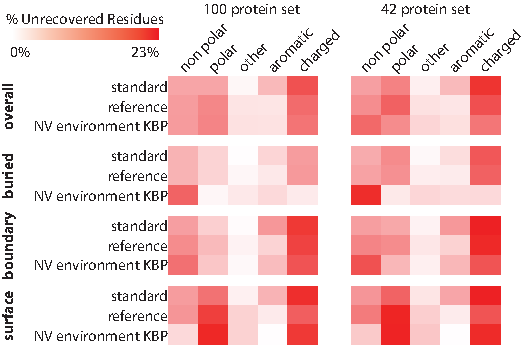
\includegraphics[width=4in]{figures/nv_kbp/recovery_by_group}
\caption{
Percentage of unrecovered residues (number of recovered residues divided by total number of residues in the benchmark set) by amino acid category in the 100 and 42 protein benchmark sets.
The color scale ranges from white (small number of mistakes) to red (large number of mistakes).
In this metric, residues were grouped into the categories polar (Ser, Thr, Asn, Gln), non-polar (Ala, Val, Leu, Met, Ile), aromatic (Phe, Tyr, Trp), charged (Lys, Arg, His, Asp, Glu), and other (Cys, Pro, Gly).
A residue was counted as recovered if it was mutated to another residue within the same group.
}
\label{fig:recovery_by_group}
\end{figure}

\section{Discussion}

The results of both the 100-protein five-way cross-validation and the 42-protein independent benchmark set are consistent.
In both cases, introduction of the \ac{NV} environment \ac{KBP} into the energy function and optimization of the energy function weights lead to an overall improvement in the quality of designed sequences.
As the independent benchmark set tests an averaged scoring function that would be generally useful, the remaining analysis will focus on this benchmark set. 

\subsection{Explanation for source of observed improvements in design}
The results of the benchmarking show that, in general, structures designed using the \ac{NV} environment \ac{KBP} exhibit smaller conformation biases and more evolutionarily favorable mutations.
A detailed analysis of these results also provides some insight into the behavior of the RosettaDesign scoring function.

\subsubsection{The \acs{NV} environment \acs{KBP} energy counteracts limitations in the RosettaDesign solvation potential}
Due to the lack of an explicit water model in RosettaDesign, the standard RosettaDesign energy function is dominated by the solvation free energy potential.
As a result, there are few constraints on amino acid mutations on the protein surface.
Due to this lack of constraints, proteins designed with the standard energy function exhibit large biases in sequence composition on the protein surface.
Proteins designed with the standard energy function show large numbers of aromatic residues on the protein surface.
Specifically, there is a 3.1\% increase in phenylalanines, a 1.9\% increase in tryptophans, and a 2.5\% increase in tyrosines on the protein surface in the benchmark set designed with the standard RosettaDesign energy function compared to the native structure.
Proteins designed with the \ac{NV} environment \ac{KBP} show a large reduction in these biases.
Proteins designed with the \ac{NV} environment \ac{KBP} showed a 1.4\% increase in phenylalanines, 0.8\% increase in tryptophans, and 1.5\% increase in tyrosines compared to native proteins.
While still large, these biases are much smaller than the biases observed with the standard energy function. 

\subsection{The \acs{NV} environment \acs{KBP} term improves design of buried residues as well as surface residues}
It was expected that improvements in the quality of surface sequence design would be the primary benefit of the \ac{NV} environment \ac{KBP}.
However, an analysis of the overall \ac{PSSM} recovery, sequence recovery, and sequence composition biases suggest that the improvement given by the \ac{NV} environment \ac{KBP} implementation occurred across the board rather than merely at the protein surface.
Table \ref{table:burial_42} shows the overall impact of the \ac{NV} environment \ac{KBP} at various levels of burial.
The percent \ac{PSSM} recovery improved using the \ac{NV} environment \ac{KBP} by 8.0\% in the buried region, 9.6\% in the boundary region, and 8.5\% on the surface region compared to the standard energy function.
The percent sequence recovery improved by 2.0\% in the buried region, 3.2\% in the boundary region, and 4.6\% in the surface region compared to the standard energy function.
 
 When percent sequence recovery is broken down by group (Figure \ref{fig:recovery_by_group}), a large increase in the recovery of buried charged residues is observed, with a 6.2\% increase compared to the standard energy function. 
 Additionally, a 3.8\% increase in recovery of non-polar residues is observed on the surface.
 Not all groups show improvement, and this is expected, as the scoring function was not directly optimized for percent sequence recovery.
 
While the overall percent changes are relatively small, these changes are both statistically and scientifically significant.
To assess the statistical significance of the data, standard deviations were calculated in tables \ref{table:100_protein_stdev} and \ref{table:42_protein_stdev}.
The standard deviations were calculated for both percent \ac{PSSM} recovery and percent sequence recovery.
Each of the five scoring functions generated during the five-way cross validation weight optimization using 100 proteins was used to design the independent set of 42 proteins.
The standard deviations of \ac{PSSM} and sequence recovery are listed in supplementary tables \ref{table:100_protein_stdev} and \ref{table:42_protein_stdev}.
The standard deviations range from 0.1-1.2\%. 
The average error is 0.4\% and therefore smaller that the improvements in recovery rates observed. 

\begin{table}
\scriptsize
\renewcommand{\tabcolsep}{0.09cm}
\centering
%This was table T3

\begin{tabular}{|r|r|r|r|r|r|r|}
\hline
 & \multicolumn{3}{c}{Percent PSSM Recovery} & \multicolumn{3}{|c|}{Percent Sequence Recovery}\\
\hline
  & Standard & Reference & NV environment KBP & Standard & Reference & NV environment KBP \\
\hline
Buried & 8.9\% & 8.9\% & 8.4\% & 11.6\% & 10.8\% & 10.1\%\\
\hline
Boundary & 9.6\% & 11.7\% & 9.2\% & 10.7\% & 11.3\% & 11.2\%\\
\hline
Surface & 8.1\% & 6.6\% & 6.9\% & 7.0\% & 8.0\% & 7.9\%\\
\hline
Overall & 6.3\% & 6.0\% & 5.2\% & 7.0\% & 7.1\% & 6.5\%\\
\hline
\end{tabular}
\caption{Standard deviations for 100 protein benchmark set data. shown in table \ref{table:burial_100}}
\label{table:100_protein_stdev}
\end{table}

\begin{table}
\scriptsize
\renewcommand{\tabcolsep}{0.09cm}
\centering
%This was table T4

\begin{tabular}{|l||r|r|r|r|r|r|}
\hline
 & \multicolumn{3}{c}{\textbf{Percent PSSM Recovery}} & \multicolumn{3}{|c|}{\textbf{Percent Sequence Recovery}}\\
\hline
  & \textbf{Standard} & \textbf{Reference} & \textbf{NV environment KBP} & \textbf{Standard} & \textbf{Reference} & \textbf{NV environment KBP} \\
\hline
\hline
Buried & 7.1\% & 6.7\% & 5.9\% & 8.1\% & 8.9\% & 7.7\%\\
\hline
Boundary & 9.2\% & 9.1\% & 8.7\% & 8.1\% & 8.0\% & 8.6\%\\
\hline
Surface & 6.9\% & 6.6\% & 7.4\% & 4.7\% & 6.8\% & 6.0\%\\
\hline
Overall & 5.5\% & 5.7\% & 5.7\% & 4.6\% & 5.5\% & 5.3\%\\
\hline
\end{tabular}
\caption{Standard deviations for 42 protein benchmark set data. shown in table \ref{table:burial_42}}
\label{table:42_protein_stdev}
\end{table}

\subsection{Sequence recovery values are near the expected maximum}
It is important to consider not only the absolute change in percent recovery, but also the change relative to the maximum possible recovery value.
In the case of sequence recovery, the maximum possible sequence recovery can be estimated by analyzing the amino acids tolerated in each position in \ac{BLAST} derived \ac{PSSM}s.
In this case, the average percentage of time that the native residue is seen in the \ac{PSSM} is used as an estimate for expected sequence recovery.
For the 100 protein benchmark set, the average was 34\%, with a standard deviation of 12\%, while in the 42 protein benchmark set, the average was 34\% with a standard deviation of 7\%.
While the achievable sequence recovery is somewhat higher due to the correlation between individual positions, these values suggest that obtaining sequence recovery rates of 40-50\% would approach the maximum.
Tables \ref{table:burial_100} and \ref{table:burial_42} show that for the 100 protein benchmark set, total overall sequence recovery is 45.7\% with the standard energy function and 47.0\% with the \ac{NV} environment \ac{KBP}.
For the 42 protein benchmark set, total overall sequence recovery is 35.7\% with the standard energy function and 38.9\% with the \ac{NV} environment \ac{KBP}.
This explains the relatively small increases in sequence recovery, as current recovery values are approaching the practical maximum.
For that reason we introduce the \ac{PSSM} recovery metric.
In this context it is important to note that the scoring functions were not directly optimized for sequence recovery but rather \ac{PSSM} recovery.
As a result, it is not surprising that the sequence recovery is not necessarily maximized during optimization. 

\subsection{PSSM recovery values improve substantially overall}
In the case of \ac{PSSM} recovery, it is reasonable to expect that 100\% \ac{PSSM} recovery is unreachable as evolution might not have sampled all amino acids tolerated in a sequence position.
A more realistic value for maximum possible \ac{PSSM} recovery is between 80\% and 90\%, though the exact value of this upper bound is difficult to estimate. \ac{PSSM} recovery with the standard energy function was 72.0\%.
The observed increase to 77.2\% with the \ac{NV} environment \ac{KBP} represents a substantial increase relative to the 80-90\% maximum and the 72\% starting point.
Generally, improvements in sequence recovery rates have been moderate when altering the energy function \citep{Kortemme:2003td}, as the major contributors to the overall energy are already fine-tuned and remain unaltered. 

Comparison of \ac{PSSM} and sequence recovery results between the 42 protein benchmark set and the 100 protein set illustrates that the performance of the RosettaDesign algorithm varies based on the characteristics of the protein being designed.
For example, Table \ref{table:burial_100} and \ref{table:burial_42} show the overall sequence recovery for proteins designed with the standard energy function.
The overall recovery for the 42 protein benchmark set was 35.7\%, while the overall recovery for the 100 protein benchmark set was 45.7\%.
This substantial difference is likely a result of the different criteria used to select the proteins in each set.
The proteins in the 42 protein benchmark set are larger than those in the 100 protein set, and will therefore have a larger total surface area and thus be more challenging targets for design.

\subsection{The sequence recovery values observed are realistic, given previous values reported in the literature}
Despite the differences inherent to different design targets, these values are similar to those obtained in the literature.
Schneider et al. designed a set of proteins of size between 89-223 amino acids based on high resolution crystal structures.
They observed surface sequence recovery rates of 22\% $\pm$ 11\%, and buried recovery rates of 56\% $\pm$ 13.7\% when designing with RosettaDesign \citep{Schneider:2009ig}.
These values are similar to those seen in Tables \ref{table:burial_100} and \ref{table:burial_42}.
Additionally, Sharabi et al. reported overall sequence recovery values of between 40\% and 70\% depending on the weights of the scoring function used during their design \citep{Sharabi:2011ev}.
These numbers are within the range of the sequence recovery values obtained during the experiments described in this manuscript.

\subsection{\acs{NV} environment \acs{KBP} term reduces sequence bias}
In addition to improvements in \ac{PSSM} and sequence recovery, the degree of sequence bias seen in the buried and boundary regions of designs made using the \ac{NV} environment \ac{KBP} decreased.
When all residues in the benchmark set are considered, proteins designed with the \ac{NV} environment \ac{KBP} have an \ac{RMS} percent composition change of 2.8\% compared to the native protein, while proteins designed with the standard energy function have an \ac{RMS} percent composition change of 2.9\% (Figure \ref{fig:overall_independent_changes}A).
When this overall value is broken down by region, the buried region designed with the \ac{NV} environment \ac{KBP} shows an increase in \ac{RMS} percent composition change compared to the standard energy function from 4.2\% to 4.5\%, the boundary region shows a decrease from 3.4\% to 2.7\%, and the surface region shows a reduction from 2.9\% to 2.4\%.
While the improvements in sequence composition bias are minimal, Figure \ref{fig:overall_independent_changes}B shows an increase in \ac{RMS} per residue \ac{PSSM} recovery from 3.8\% with the standard energy function to 4.2\% with the \ac{NV} environment \ac{KBP}.
Additionally, Figure \ref{fig:overall_independent_changes}C shows an increase in \ac{RMS} per residue sequence recovery from 2.4\% with the standard energy function to 2.6\% with the \ac{NV} environment \ac{KBP} energy function, which is expected given the optimization of the scoring function towards \ac{PSSM} improvement. 

\begin{figure}
\centering
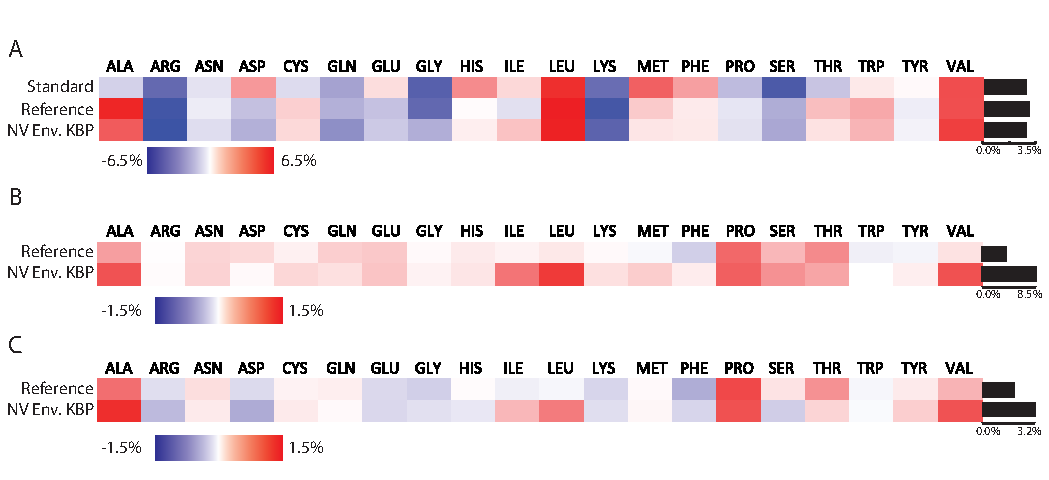
\includegraphics[width=4in]{figures/nv_kbp/overall_independent_changes}
\caption{
A) shows the percent change in overall sequence composition between native and designed proteins for all 42 structures in the independent benchmark set.
The black bars show the \acs{RMS} percent composition change. 
B) shows the percent \acs{PSSM} recovery for all 42 structures in the independent benchmark set.
The black bars show \acs{RMS} percent \acs{PSSM} recovery.  
C) percent sequence recovery for all 42 structures in the independent benchmark set.
The black bars show \acs{RMS} percent sequence recovery.
}
\label{fig:overall_independent_changes}
\end{figure}

\subsection{Addition of the \acs{NV} environment \acs{KBP} term results in reduction of solvation term weight}
An investigation of the optimized weights lends some insight into the cause of the improvements in sequence design.
 Table \ref{table:energy_weights} and \ref{table:ref_energy_weights} show the scoring function and reference energy weights of the standard energy function and the optimized \ac{NV} environment \ac{KBP}.
When the \ac{NV} environment \ac{KBP} term is added to the energy function, the weight of the free energy solvation potential decreases from 0.65 in the standard energy function to 0.56 in the \ac{NV} environment \ac{KBP}. 
The \ac{NV} environment \ac{KBP} term has a value of 1.01.
As discussed earlier, in the standard energy function, the reference energies and solvation free energy potential are the dominant forces on surface residues due to the lack of explicit inter-residue interactions.
Because the penalty given by the solvation free energy potential for apolar residues on the surface is relatively weak, the weight of this potential will need to be increased for it to adequately effect surface residues.
However, because the energy function is applied evenly, regardless of degree of burial, the increase in weight necessary to maintain a reasonable protein surface may cause the solvation free energy potential to apply too strongly to the boundary region.
As the burial level increases, the number of inter-residue interactions will also increase, which explains the decrease in improvement in sequence bias seen at more highly buried regions of the protein.
This idea is supported by the decrease in free energy solvation potential weight observed in the \ac{NV} environment \ac{KBP} energy function.
The \ac{NV} environment \ac{KBP} provides additional information about protein surface composition, reducing the dominance of the free energy solvation potential.

\begin{figure}
\centering
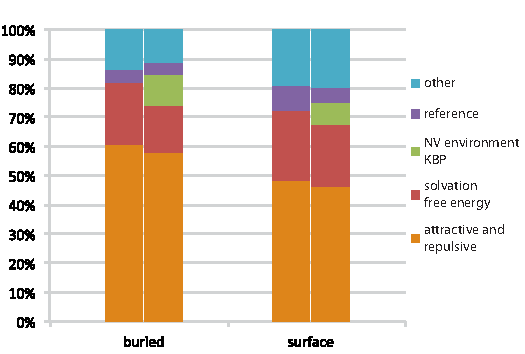
\includegraphics[width=4in]{figures/nv_kbp/term_contribution}
\caption{
The contribution of individual scoring terms towards the overall score of buried and surface residues.
The introduction of the \acs{NV} environment \acs{KBP} reduces the reliance on solvation free energy and the attractive/repulsive forces at both levels of exposure. 
}
\label{fig:term_contribution}
\end{figure}

\subsection{The \acs{NV} environment \acs{KBP} term reduces the influence of the solvation term on total score}
Figure \ref{fig:term_contribution} shows the effect of the \ac{NV} environment \ac{KBP} on the overall scoring function.
All proteins used in the 100 protein benchmark set were scored using both the standard RosettaDesign energy function and the optimized \ac{NV} environment \ac{KBP} energy function. 
The average magnitude of each scoring term for each buried and surface residue was calculated, and converted to percentage of the total energy for each residue to measure the influence of each scoring term.
We observe that the addition of the \ac{NV} environment \ac{KBP} term decreases the influence of the reference energies, solvation free energy term, and the attractive and repulsive terms throughout all degrees of burial.
Specifically, the influence of the solvation free energy decreases from 21\% to 16\% for buried residues, and from 24\% to 21\% for surface residues.
Additionally, the influence of the reference energy decreases from 8\% to 5\% on the surface, though it remains relatively unchanged for buried residues.
The attractive and repulsive forces also change somewhat, with a decrease in influence from 60\% to 57\% in buried residues, and 48 to 46\% in surface residues.
This change in influence is significantly less than the change in influence seen in the reference and solvation free energy functions.
The \ac{NV} environment \ac{KBP} was designed to address shortcomings in the design of the protein surface.
These shortcomings are the result of the energy function failing to model aspects of the protein surface that are not completely described through the solvation and reference energies.
To achieve reasonably good performance despite these inaccuracies, both energy terms are overweighted in the standard energy function.
As expected, addition of the \ac{NV} environment \ac{KBP} term reduces the impact of solvation and reference energies on the surface.
As these adjustments apply throughout all degrees of burial, the artificially inflated weight of the solvation and reference energies can be decreased, improving performance also in the buried regions of the protein as well.

\subsection{The \acs{NV} environment \acs{KBP} term may encode environmental effects reducing aggregation potential}
In addition to providing information about solvation effects, the \ac{NV} environment potential also sheds light on the evolutionary and environmental forces on protein composition.
Soluble proteins have evolved to be non-aggregative and generally stable in the environment of a cell.
These properties are difficult to model via physics-based methods, as they arise from numerous inter-protein interactions that are difficult to explicitly model.
The implicit modeling of these environmental effects accounts in part for the improvements in native-like sequence design seen during design with the \ac{NV} environment \ac{KBP}.
By optimizing the \ac{NV} environment \ac{KBP} energy function to maximize \ac{PSSM} score rather than sequence recovery, the energy function is optimized to design proteins similar to those which are favored evolutionarily, rather than to merely reproduce the native sequence.
%\chapter{Improving RosettaLigand Speed and Sampling Efficiency through the Development of a Novel Sampling Algorithm}
\label{chap:lowres_paper}
\section{Abstract}

RosettaLigand has been successfully used to predict protein-ligand binding poses in a number of cases\citep{Turlington:2013et,Davis:2009fx,Combs:2013bl}.
However, the RosettaLigand docking protocol is relatively inefficient at sampling the ligand binding site space, making it unfeasibly slow for use as a virtual High Throughput Screening (vHTS) tool.
We show here that the development of a new sampling algorithm for initially placing the ligand in the protein binding site dramatically improves both the overall success rate of small molecule docking as well as speed of RosettaLigand.
The new algorithm improves the docking success rate by 10-15\% in a 43 protein benchmarking set, reduces the average time to generate a model from 50 seconds to 10 seconds, and reduces the necessary number of models to generate from 1000 to 150.
We also demonstrate that accurate initial placement of the ligand prior to full atom refinement is critical to successful prediction of an accurate binding pose.

\section{Introduction}

\subsection{Ligand docking background}

\subsubsection{Ligand docking background}

Computational ligand docking has been a historically successful method for predicting the binding pose of small molecules in a protein.
Beginning with PJ Goodford's work in computational drug design\citep{Goodford:1985bf}, many methods have been developed to predict the interactions between proteins and small molecules.
While early tools focused primarily on rigid body goodness of fit between a small molecule and a protein crystal structure, further study of the changes observed in protein conformation upon the binding of a small molecule\citep{Bystroff:1991tl} suggested that modeling of protein and ligand flexibility was important to correctly model protein-ligand interactions.

\subsubsection{An overview of popular ligand docking tools}

Over the past several decades, numerous tools have been developed to attempt to better address the ligand docking problem.
DOCK\citep{Ewing:2001wu}, FlexX\citep{Hindle:2002tk}, AutoDock\citep{Morris:1998vi}, and Glide\citep{Friesner:2004hm} are currently among the most popular tools.
They utilize a wide range of protein representations, sampling algorithms and scoring functions in order to accurately predict protein-ligand binding poses.
Approximations in scoring and sampling must be made in order to allow ligand binding predictions to be made in a reasonable time.
To accomplish this, most ligand docking tools operate in stages, so that the size of the search space is limited as the complexity of the scoring function and sampling density within the search space is increased.

\subsubsection{Summary of popularly used docking algorithms}
Docking methods differ in their means of accomplishing this step-wise increase in sampling resolution coupled with the reduction of search space.
For example, the DOCK algorithm creates a "negative space" model of the binding site created by placing spheres inside the solvent accessible area of the binding site, and uses this model to guide docking of the ligand, while an AMBER based molecular mechanics force field is used to score the resulting binding poses\citep{Moustakas:2006fe}.
FlexX, on the other hand, represents the protein by "interaction centers" consisting of surfaces surrounding common ligand interaction groups (hydrogen bond donors and acceptors, metals, aromatic rings, etc.).
Atoms in a based fragment of the ligand are then matched to the interaction centers to provide an ensemble of potential initial placements\citep{Rarey:1996hf}.
AutoDock represents the receptor using a Cartesian scoring grid populated with information from an empirically derived energy function.
A Lamarckian Genetic Algorithm (LGA) in combination with simulated annealing is then used to optimize both the ligand conformation and position\citep{Morris:1998vi}.
Glide uses a grid based representation of the protein binding site. A rapid exhaustive search is first performed to find generally favorable areas for ligand placement.
A size filter is then used to exclude areas without sufficient space for ligand placement.
Finally, Monte Carlo Minimization (MCM) of the binding pose using the grid based scoring function is performed.
The scoring girds themselves are generated using a scoring function derived from ChemScore\citep{Friesner:2004hm}.

\subsection{Performance comparison}

\subsubsection{Performance of ligand docking tools is inconsistent} 
Despite the large differences between scoring and sampling algorithm implementations across the different ligand docking tools, a blind study of ligand docking performance conducted by Davis et al.\citep{Davis:2009fx} suggested that while certain methods of docking perform better than others for a given protein target, in the aggregate, the commonly used systems have a similar range of performance.
Interestingly, while some protein systems appear to be relatively easy (Chk1 kinase) or difficult (Hepatitis C RNA Polymerase) for most ligand docking tools, the results for most systems vary depending on the ligand docking tool.

\subsection{Limitations of the RosettaLigand low resolution docking step}

\subsubsection{Introduction to the RosettaLigand docking process}
As currently implemented, RosettaLigand consists of a two stage docking process consisting of an initial placement stage followed by a refinement stage.
The overall effect of the initial placement algorithm is to place the ligand in a non-clashing position at random.
To accomplish this, the initial placement algorithm consists of three steps, which were initially described in Davis et al.\citep{Davis:2009bf}
The algorithm uses a binary scoring grid to identify non-clashing regions of the protein.
The binary scoring grid consists of "attractive" rings between 2.25 and 4.75 \AA\ of every heavy atom, and ?repulsive? spheres between 0 and 2.25 \AA\ of each backbone heavy atom. 
The first step of the initial placement algorithm ("Translate") consists of up to 50 random translations within 5.0 \AA\ of the starting position.
After each translation, the heavy atom closest to the geometric center of the ligand, termed the ?neighbor atom? is scored using the binary scoring grid.
If the score is -1 or 0 (attractive or neutral), move is accepted, and the translation step terminates.
The aim of the Translate step is to place the ligand in a region of the binding site that is not majorly clashing.

\subsubsection{Description of the Rotate step}
The second step in the initial placement algorithm is the Rotate step.
The Rotate step consists of up to 500 random rotations with a maximum of 360\textdegree\ from the starting orientation.
The Rotate step accumulates a set of diverse non-clashing ligand orientations, and then selects one of these orientations at random for further refinement.
The size of the set of diverse orientations is either 5 or 5 times the number of rotatable bonds in the ligand, whichever is larger.
The ligand is randomly reoriented, and then accepted into the set of diverse orientations if the following conditions are met: No atoms are located in repulsive squares, 85\% of the atoms are located on attractive squares, and the RMS of the new orientation with respect to all previously accepted conformations is greater than $0.65*\sqrt{number\ of\ heavy\ atoms}$.
After either 500 orientations have been created, or the maximum set size has been achieved, a random orientation from the set is selected, and the Rotate step terminates.

\subsubsection{Description of the Slide Together step}
The third and final step in the initial placement algorithm is the Slide Together step.
Due to the relatively small amount of information provided by the binary scoring grid, it is possible for the ligand to be placed in a region where it does not contact any protein atoms at the end of the translate and rotate steps.
In this case the apparent interaction energy at the beginning of the refinement stage would be 0, reducing the efficiency and sometimes causing failure in the following Monte Carlo refinement stage.
To avoid this situation, the ligand must be brought in contact with the protein.
The Slide Together step moves the ligand towards the center of mass of the protein until the full atom repulsive score increases. 
Following this initial placement, a refinement stage is carried out in which small perturbations of the ligand and repacking of the protein side-chains are performed using MCM.
Finally, all atoms in the binding site are minimized using gradient minimization, and the final structure is scored.

\subsubsection{Possible limitations of the low resolution placement in RosettaLigand}
We hypothesize that independent sampling of translation and rotation will complicate sampling of all favorable initial placements, particularly if the ligand is not globular.
For example a rod-shaped ligand would easily enter a rod-shaped pocket but only if it is brought in the correct orientation first.
A ligand with a bent shape might require reorientation while entering the binding pocket in order to avoid clashes.
Therefore, RosettaLigand will miss out on favorable initial placements for other ligands but spend substantial time performing refinement and minimization moves on ligands placed in unfavorable initial positions.
The result of this inefficiency would be an increased failure rate as some ligands are never placed in favorable starting positions, and for other ligands an effectively increased runtime, as the number of ligand poses which must be generated to reliably produce a high quality binding pose is increased.
Lemmon et al.\citep{Lemmon:2013jd} determined that as many as 1000 models may be necessary to produce at least one high quality binding pose in a challenging docking case.
Given this, improving the efficiency of protein binding site sampling by starting from more favorable initial placements has the potential to drastically reduce the computational cost of RosettaLigand, allowing for a larger number of predictions to be made given a fixed amount of computing resources.

\section{Results}

The improved initial placement algorithm has two components: A modular grid based scoring function, and a MCM based sampling algorithm.
Both components are fully independent.
The implementation described here allows for the rapid implementation of new score terms and sampling methodologies, and the easy integration of these methods into the existing RosettaLigand pipeline.

\subsection{Score function development}
\subsubsection{Description of scoring grids and manager}

The new score function consists of a set of scoring grids which are controlled by a scoring manager.
Each scoring grid is responsible for computing a single term in the energy function.
It consists of a 3D tensor of floating point values representing Cartesian space.
It also contains functions to populate that tensor, and to score a ligand positioned in that tensor.
The scoring manager is responsible for keeping every scoring grid up to date with respect to the protein pose, and for making sure that the ligand is scored in every grid.
Additionally, the scoring manager is responsible for handling the weighting of the individual scoring terms to compute the total score.
For this study, the tensor has dimensions of 15 \AA$^{3}$ width, and a 0.25 \AA\ spacing between grid points. 

\subsection{Sampling architecture}
\subsubsection{Description of grid MCM}
An MCM algorithm is used to compute the initial binding pose for the ligand.
Figure \ref{fig:docking_flowchart} shows a flow chart of the overall steps in the sampling process.
At each step in the sampling process the ligand is either randomly perturbed in the binding site, or the conformation of the ligand is changed.
Ligand perturbation is performed as a combination of a random translation and rotation, and the conformation of the ligand is perturbed by selecting a random conformation from a library of pre-computed conformers.
After the perturbation, the ligand is scored using the scoring grids described above, and, the Metropolis criterion is applied to either accept or reject the new pose.
500 cycles of sampling are performed, and the best scoring ligand pose is saved.
During sampling, only the scoring grids are used to provide scoring information, and the protein is therefore rigid.
By only using scoring grid information, it is possible to perform 500 cycles of sampling in roughly 1-3 seconds.

\begin{figure}
%figure 1 in orginal paper
\centering
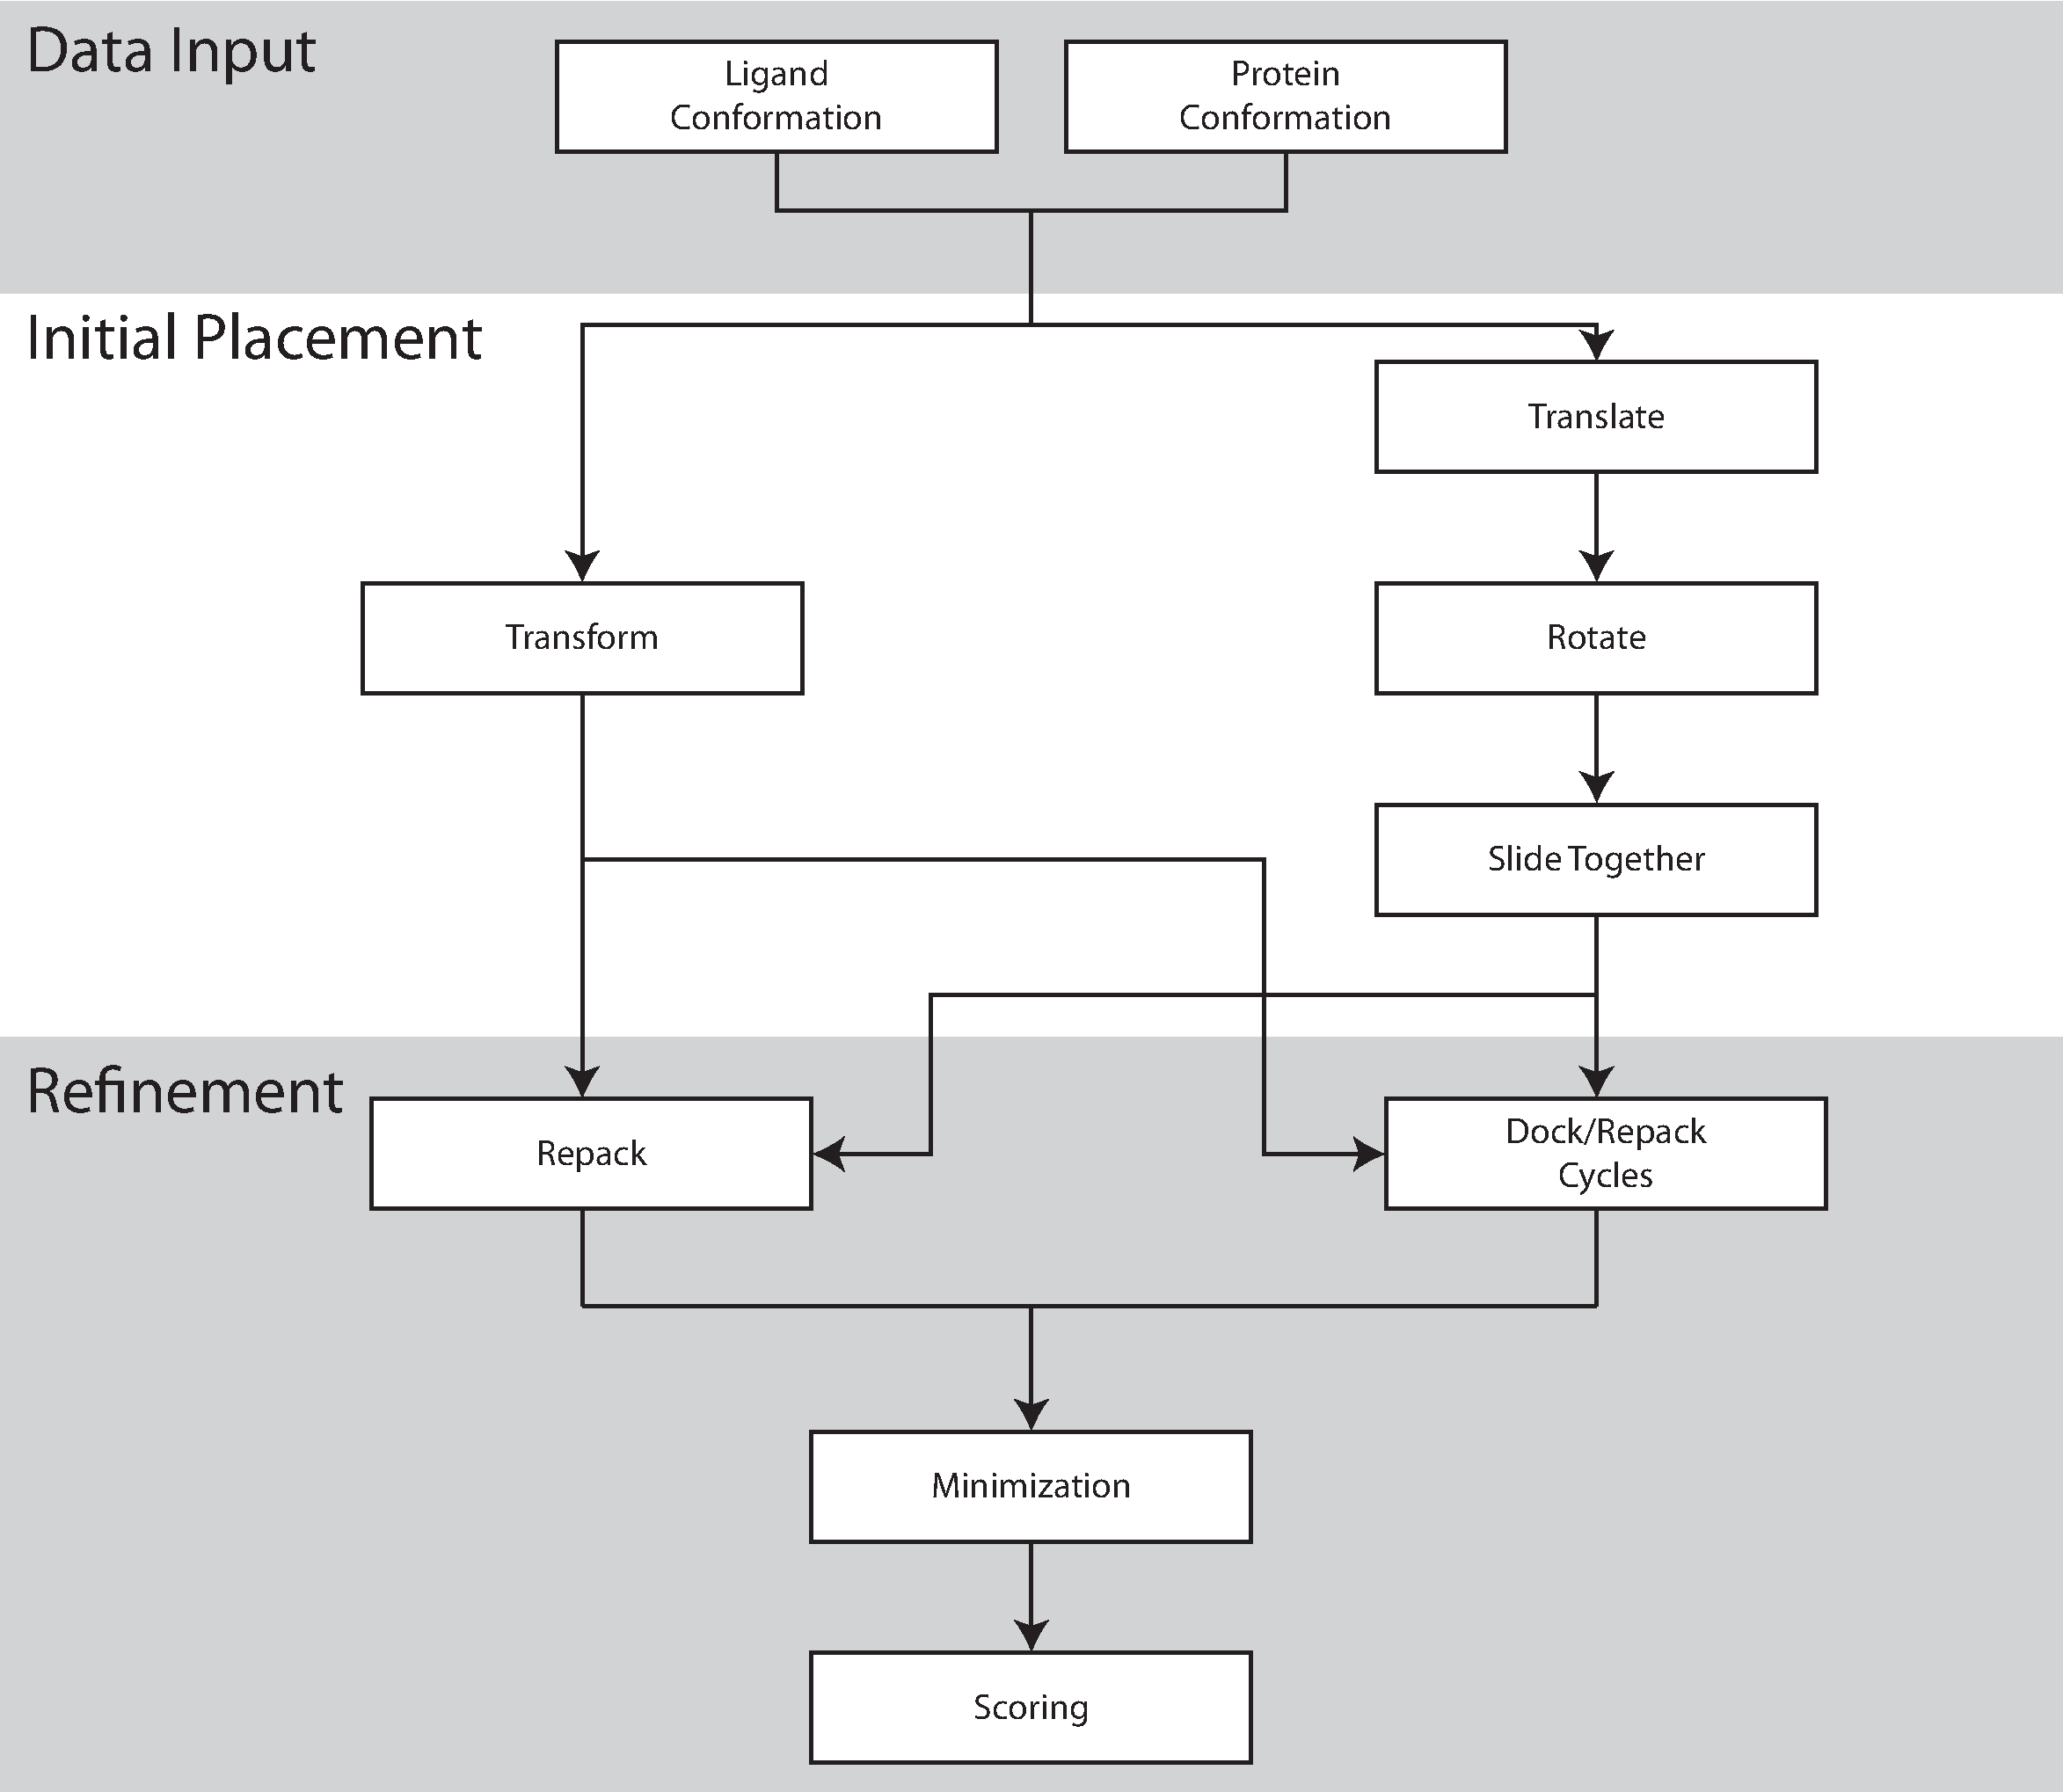
\includegraphics[width=4in]{figures/lowres/protocol_flowchart.pdf}
\caption{
A general schematic of the docking protocols described in this paper.
Because the initial placement and refinement steps are independent, the two initial placement algorithms can be combined to produce a total of four ligand docking algorithms.  
}
\label{fig:docking_flowchart}
\end{figure}

\subsection{Docking Protocol}
\subsubsection{Introduction to the docking process}
The overall docking protocol is illustrated in the schematic flowchart in Figure \ref{fig:docking_flowchart}.
The study compares different configurations of both the initial placement step and the refinement step, described below.
Complete RosettaScripts XML files for each experiment can be found in the supplementary information.
As a baseline we use the \textsc{TransRot} initial placement algorithm, where translation and rotation moves are performed separately using the binary scoring grids described by Davis et al.\citep{Davis:2009bf} and summarized in the introduction.
The specific TransRot protocol used here is originally described in Fleishman et al.\citep{Fleishman:2011ji}, and is conceptually identical to the process described in the Davis paper, though the user interface is different. 

\subsubsection{Description of the \textsc{Transform} based initial placement algorithm}

In the new \textsc{Transform} based initial placement algorithm, translation and rotation are performed simultaneously.
500 steps of MCM are carried out.
At each step, the ligand position is either transformed, or the ligand conformation is changed using the ligand conformers described above.
When a transformation move is selected, the ligand is randomly translated within 0.1 \AA\ of its current position, and rotated within 5\textdegree.
The ligand is constrained to only move within 5 \AA\ of the starting position.
After each move, the score is evaluated as the sum of the values at each grid square occupied by a ligand atom.
The move is the accepted or rejected using the Metropolis criterion, and the best scoring accepted move after all 500 steps is returned.

\subsubsection{Description of the MCM refinement algorithm}
During MCM refinement, the scoring grids are not used, and the full atom Rosetta energy function is used for energy computation.
MCM refinement consists of two steps: high resolution docking, and gradient-based minimization.
Six steps of high resolution docking are performed. The steps consist of either repacking followed by minimization, or ligand perturbation.
In the repacking and minimization step, the side-chain positions are optimized using side-chain rotamers from the Dunbrack rotamer library\citep{Shapovalov:2011bw}, and the ligand is allowed to change conformation using the pre-computed ligand conformers.
Following repacking, a gradient based minimization is applied to minimize the energy of the side-chain and ligand atoms.
In the perturbation step, the ligand is randomly perturbed within a range of 0.1 \AA\ and rotated within a range of 5\textdegree.
The two moves are alternated such that the first, third and final moves are repacking and minimization, while the remaining are ligand perturbations. The six moves are performed using a MCM algorithm, and the best scoring pose of the six moves is selected.
After the high resolution docking step, a final minimization is carried out in which the protein side-chain and backbone atoms in the binding site, as well as the ligand atoms, are all minimized using a gradient based minimization.

\subsubsection{Description of MIN refinement}
MIN refinement is carried out similarly to MCM refinement, except in the case of MIN refinement, only a single round of repacking is performed prior to the final minimization.
Because no ligand perturbation is performed during MIN refinement, the ligand pose generated during in the initial placement stage becomes critical.

\subsection{Benchmarking setup}
\subsubsection{Introduction to benchmarking scheme}
To benchmark the performance of the new initial placement algorithm, a docking benchmark derived from the CSAR\citep{DunbarJr:2011kq} dataset was used.
A subset of 43 proteins from the CSAR data set was used (Supplemental table). % TODO: add supplement
This subset omits protein/ligand complexes with co-factors, metal ions, or water molecules that bridge ligand and protein.
While Rosetta has successfully been used in such cases\citep{Lemmon:2013jd},  the inclusion of critical waters, co-factors or metal ions greatly increases the number of degrees of freedom in the docking simulation, which in turn would make the results of benchmarking more complex to interpret.
 
\subsubsection{Description of the three sets of input proteins used for benchmarking}
Because the new initial placement algorithm relies on a pre-computed scoring grid, the initial positions of the protein atoms are going to have an effect on the quality of the generated binding poses.
To assess this impact, three sets of input structures were used in docking: The crystal structures provided in the CSAR dataset, repacked structures in which the backbone was held fixed and the side-chains re-optimized without the co-crystallized ligand present, and relaxed structures in which both the side-chain and backbone atoms were minimized in absence of the small molecule.
In the case of the crystal and repacked structures, only a single protein structure was used for docking. In the case of the relaxed structures, the ligand was docked into an ensemble of ten models. 

\subsubsection{Twelve benchmark experiments were performed}
Each experiment is a combination of one set of input protein structures above (crystal, repacked, or relaxed) and one docking protocol.
Four docking protocols were selected to investigate the behaviors of each component of the docking algorithms.
A docking protocol consists of an initial placement algorithm (\textsc{TransRot} or \textsc{Transform}), and a refinement algorithm (MCM or MIN).
Figure \ref{fig:docking_flowchart} is a schematic describing the overall docking process. 

\subsection{Summary of results}
\subsubsection{New method decreases amount of time to make one model}
Figure \ref{fig:time_per_model} shows the change in the average time necessary to generate a single model with each of the four tested algorithms.
The average time needed to generate a model using the previously published \textsc{TransRot}/MCM protocol is 49.4 seconds per model.
Changing the Refinement protocol from MCM to MIN reduces the time per model to 33.3 seconds, and changing both the refinement protocol to MIN and the initial placement model from \textsc{TransRot} to \textsc{Transform} further reduces the time per model to 9.3 seconds.
From this timing data we can conclude that that the majority of computational time spent by the previously published \textsc{TransRot}/MCM algorithm is split roughly evenly between the initial placement stage and the refinement stage.
A combination of the new \textsc{Transform} initial placement algorithm and MIN refinement is capable of consistently generating models approximately 5-10 times faster than the previously published docking algorithm.

\begin{figure}
%figure 2 in orginal paper
\centering
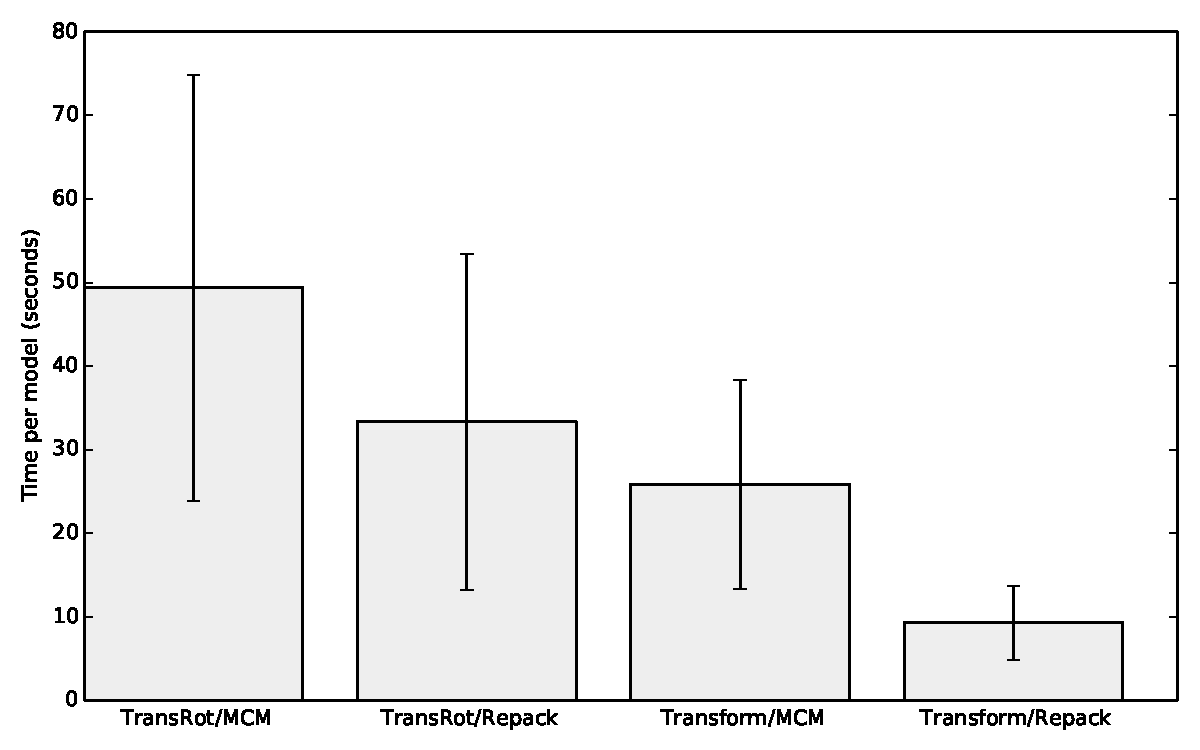
\includegraphics[width=4in]{figures/lowres/time_per_model.pdf}
\caption{
The average time and standard deviation to produce a single model for each docking algorithm and type of input pose.
\textsc{TransRot}/MCM is the algorithm previously published by Davis et al\citep{Davis:2009bf}. 
}
\label{fig:time_per_model}
\end{figure}


\subsubsection{Use of the MIN refinement algorithm improves consistency in run time compared to MCM refinement.} 
Further timing consistency is seen when the MIN refinement stage is used in place of MCM refinement.
Each round of repacking in MCM refinement requires that the interactions between atoms in the binding site be recomputed.
As the computational complexity of this operation increases with the square of the number of atoms in the protein-ligand interface, the docking of ligands into larger binding pockets takes substantially larger when using MCM refinement compared to the docking of ligands into smaller binding pockets, which contributes in the observed changes in timing consistency.

\subsubsection{The \textsc{Transform} algorithm improves docking success rate}
Figure \ref{fig:fraction_successful_time} and Figure \ref{fig:fraction_successful_time} plot the fraction of protein-ligand systems for which the lowest scoring pose is < 2.0 \AA\ RMSD as a function of CPU time and number of models generated, respectively.
These figures indicate that the choice of initial placement algorithm is far more important than choice of low resolution scoring method or refinement method.
Docking protocols which make use of the \textsc{Transform} initial placement algorithm can reliably dock an additional 10-15\% of models within roughly 15 minutes of CPU time, or 150 models, compared to protocols which use the previously published \textsc{TransRot} initial placement algorithm.
The choice of refinement algorithm appears to play little role in the overall performance of the docking protocol, except in the case of the previously published algorithm (\textsc{TransRot}/MCM), in which case docking performance begins to approach the \textsc{Transform} based protocols after roughly 800-1000 models have been generated (Figure \ref{fig:fraction_successful_time}).
This observed behavior is consistent with previously published studies of RosettaLigand performance using this protocol\citep{Davis:2009fx,Combs:2013bl,Lemmon:2012ku}. 

\begin{figure}
%figure 4 in orginal paper
\centering
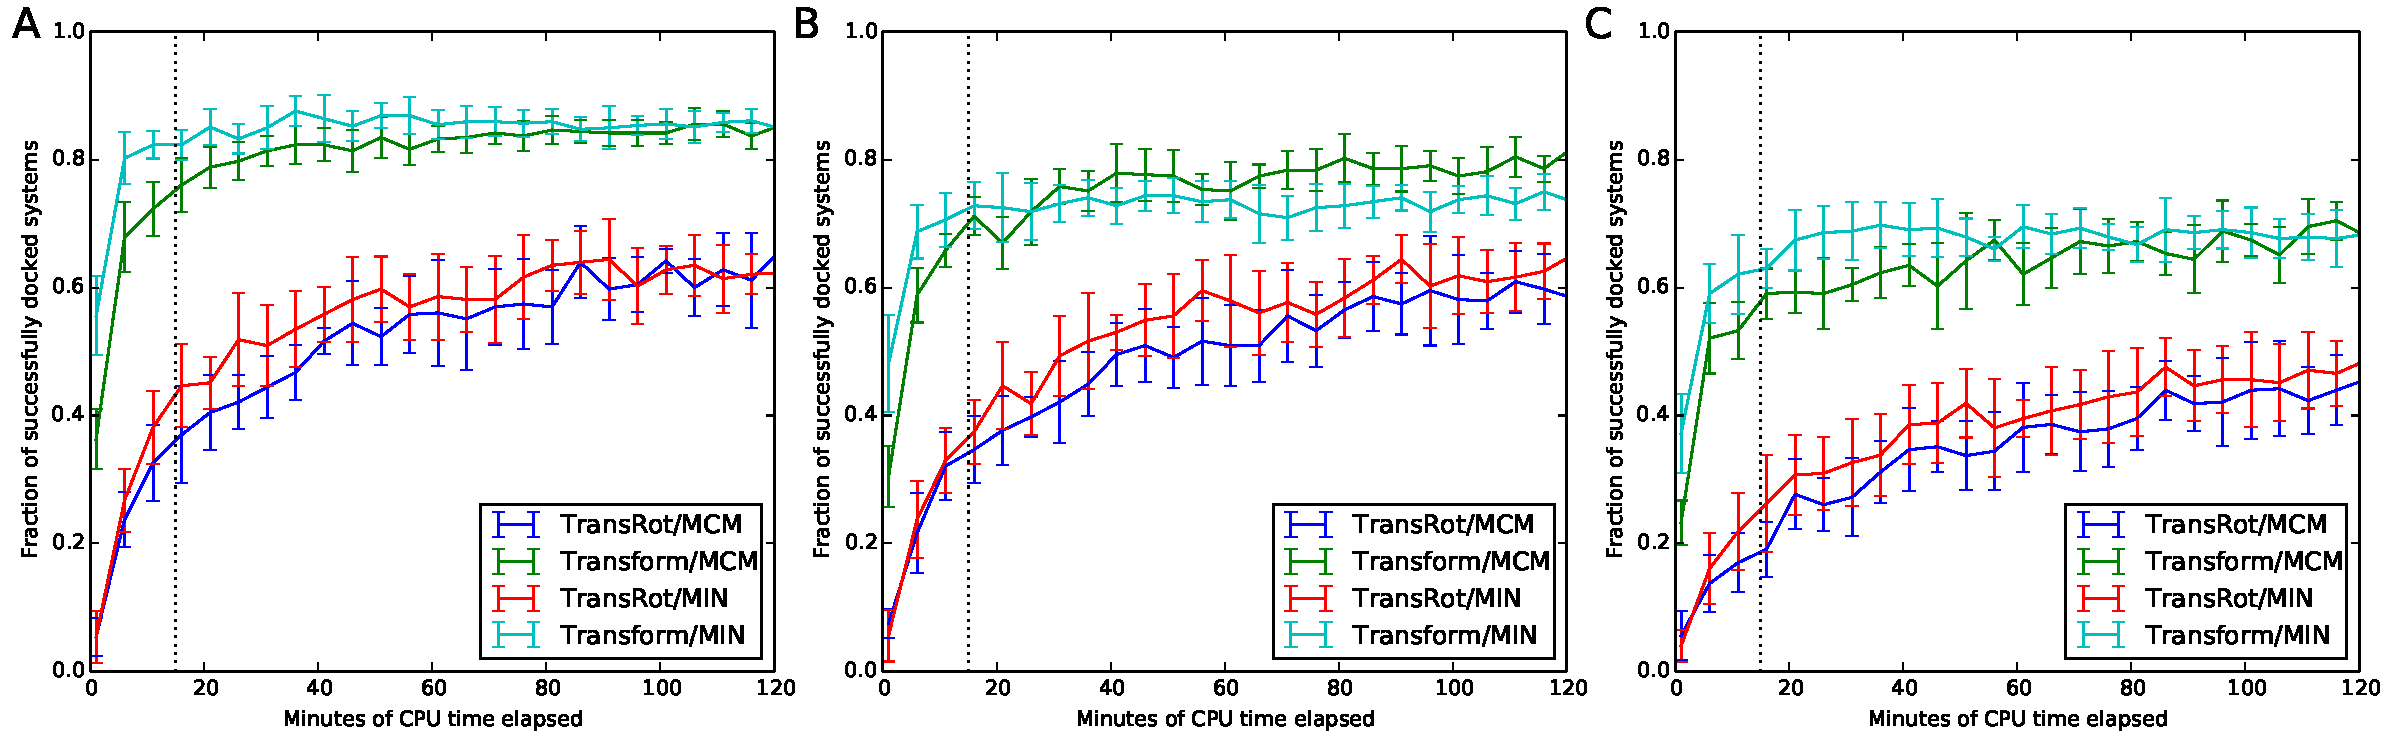
\includegraphics[width=4in]{figures/lowres/fraction_successful_time.pdf}
\caption{
The fraction of protein systems in which the lowest scoring model has an RMSD < 2.0 \AA\ to the native structure as a function of CPU time using the 3 evaluated RosettaLigand docking algorithms when docked into A) Crystal structures, B) Repacked crystal structures, and C) Relaxed crystal structures.
A large pool of models were generated, and random subsamples were taken corresponding to time points at 5 minute intervals.
The number of structures included in each time point was based on the average time to generate a model for each algorithm.
20 random samples were taken for each time point, and the means are plotted, with the error bars representing the standard deviation.
Docking protocols which make use of the \textsc{Transform}  algorithm are reliably converged after approximately 15 minutes (dotted line).
}
\label{fig:fraction_successful_time}
\end{figure}

\begin{figure}
%figure 5 in orginal paper
\centering
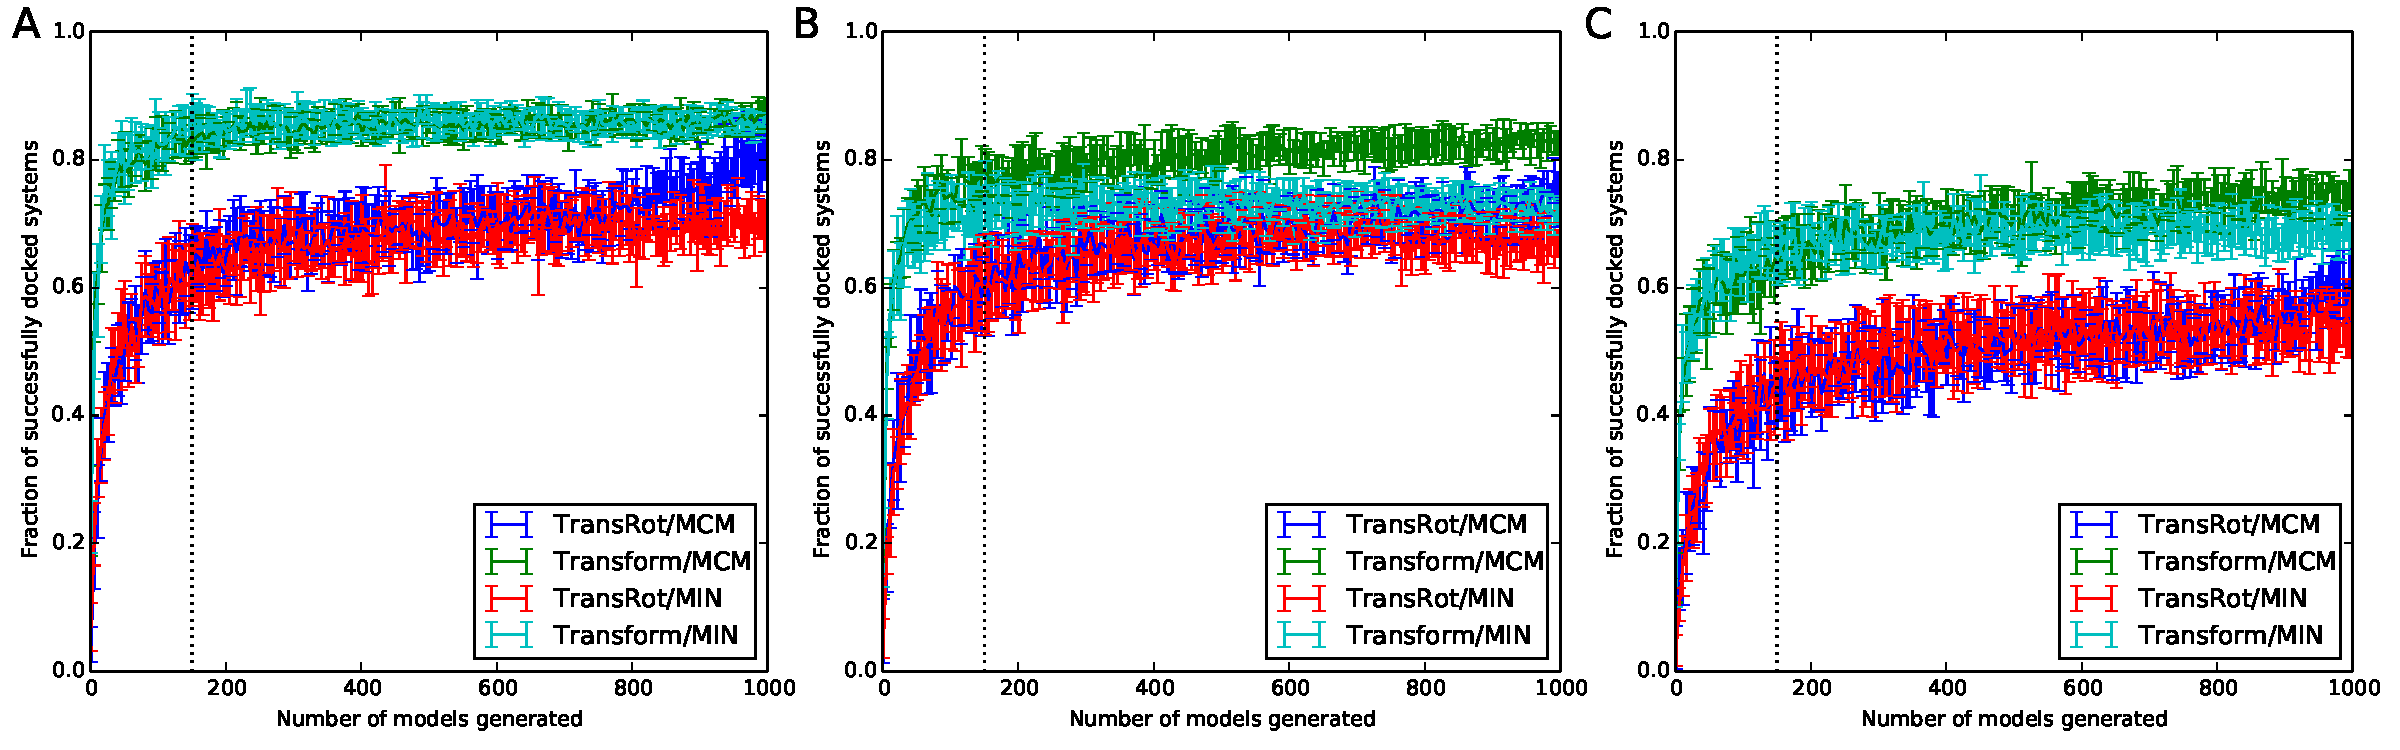
\includegraphics[width=4in]{figures/lowres/fraction_successful_count.pdf}
\caption{
The fraction of protein systems in which the lowest scoring model has an RMSD < 2.0 \AA\ to the native structure as function of the total number of structures generated using the 3 evaluated RosettaLigand docking algorithms when docked into A) Crystal structures, B) Repacked crystal structures, and C) Relaxed crystal structures.
A large pool of models were generated, and random subsamples were taken.  20 random samples were taken for each point, and the means are plotted, with the error bars representing the standard deviation.
Docking protocols which make use of the \textsc{Transform} algorithm are reliably converged after approximately 150 models (dotted line).
}
\label{fig:fraction_successful_time}
\end{figure}

\subsubsection{The new algorithm is still tolerant of backbone and side-chain perturbations}
It is clear from Figure \ref{fig:fraction_successful_time} and Figure \ref{fig:fraction_successful_time} that despite using a pre-computed scoring grid during initial placement, RosettaLigand with the new initial placement algorithm is still tolerant of changes to the side-chain and backbone conformations of the protein binding site. In all tested protocols, the success rate of RosettaLigand decreases as the uncertainty associated with the protein side-chain and backbone atoms increases.
In other words, after 1000 models have been generated docking ligands into crystal structures (Figure \ref{fig:fraction_successful_time}A), The \textsc{TransRot}/MCM protocol has successfully docked 76\% of models, while the \textsc{Transform}/MCM protocol has successfully docked 94\%.
When ligands are docked into relaxed models in which both backbone and side-chain atoms are perturbed (Figure \ref{fig:fraction_successful_time}C), The \textsc{TransRot}/MCM protocol has successfully docked 58\% of models, while the \textsc{Transform}/MCM protocol has successfully docked 84\%.
The reduction in success rate is expected because the addition of side-chain and backbone perturbation effectively adds noise to the protein structure.
However, we see that the \textsc{Transform}/MCM protocol results in a 10\% decrease in success rate between relaxed and crystal structures, rather than 18\% for the \textsc{TransRot}/MCM protocol, so the new \textsc{Transform} protocol is more tolerant of inaccurate protein structures than the original protocol.
Because the new initial placement algorithm is more likely to place the ligand in a high quality binding pose, a greater percentage of total docking time is spent in proximity or the correct binding site and pose.
As a result, the sampling density increases and thereby the overall success rate of Rosetta ligand increases relative to the \textsc{TransRot}/MCM algorithm.

\section{Discussion}

\subsection{Explanation for time decrease}
Because the rotation step of the \textsc{TransRot}/MCM initial placement algorithm used the number of rotatable bonds to determine how many rotations to perform, the amount of time required for the rotation step varies linearly with the number of rotatable bonds.
Because the \textsc{Transform} initial placement algorithm uses an MCM algorithm with a fixed number of cycles, the time to complete a single model is more consistent compared to protocols which use the \textsc{TransRot} algorithm.  

\subsection{Details of performance optimization in the \textsc{Transform} algorithm}
While the \textsc{Transform} initial placement algorithm performs roughly the same number of sampling moves during initial placement as the \textsc{TransRot} algorithm, the speed improvements seen are a result of differences in how those moves are computed.
Rosetta uses a system called the "fold tree" to represent the relationships between rigid body regions of the protein system\citep{Davis:2009bf,Das:2008gf}.
Because permutations of the protein structure made using the fold tree are performed in internal coordinate space, it is possible to rapidly modify a large system.
In the case of ligand docking, however, the system being manipulated is quite small, and the computation of fold tree based permutations quickly becomes dominated by conversions between internal and cartesian coordinate space.
Because only the scoring grids are used for pose evaluation during the initial placement step, the \textsc{Transform} algorithm represents the ligand as a list of points, which are directly transformed using a rotation and translation matrix.
This method of computing ligand permutations is substantially faster than the previous fold tree based method, and accounts for the majority of the observed speed improvement.

\subsection{The new algorithm improves sampling efficiency and speed}
Based on the results of the benchmarking studies described above, the overall effect of the new sampling algorithm is two-fold.
First, the quality of binding poses generated during the initial placement stage is improved, and second, the amount of time required to generate the initial placement is reduced.
The improvement of the poses generated by the initial placement stage results in additional speed improvements by reducing the amount of sampling necessary to produce a high quality binding pose.
The improved sampling efficiency afforded by the new initial placement algorithm both reduces the time that must be spent in high resolution docking, and reduces the total number of models which must be created to reliably produce a correct predicted binding pose.

\subsection{The majority of performance improvement is driven by the improvements to the initial placement sampling algorithm}
Figure \ref{fig:rmsd_vs_rmsd} compares the performance of several of the tested RosettaLigand protocols, and provides further insight into the impact of the various components of the protocol on overall performance.
The RMSD vs RMSD plots illustrate specific performance differences comparison between pairs of Rosetta protocols.
When the original \textsc{TransRot} initial placement algorithm is used, minimal improvement is observed when the MIN refinement algorithm is used as compared to MCM initial placement (Left).
While 17 of the 43 proteins show improvement in RMSD, only 1 exhibits sufficient improvement to cross the 2.0 \AA\ cutoff.
Comparison of the \textsc{TransRot} and \textsc{Transform} initial placement (Center) shows substantial improvement when the \textsc{Transform} initial placement algorithm is used, with 41/43 proteins having improved RMSDs, and 18/43 having enough improvement to cross the 2.0 \AA\ threshold.
Comparison of the MCM and MIN refinement algorithms when the \textsc{Transform} initial placement algorithm is used shows that in this context the two refinement algorithms have nearly identical performance (Right).
From this data we can conclude that the improvements seen are driven primarily by the new initial placement algorithm. 

\begin{figure}
%figure 3 in orginal paper
\centering
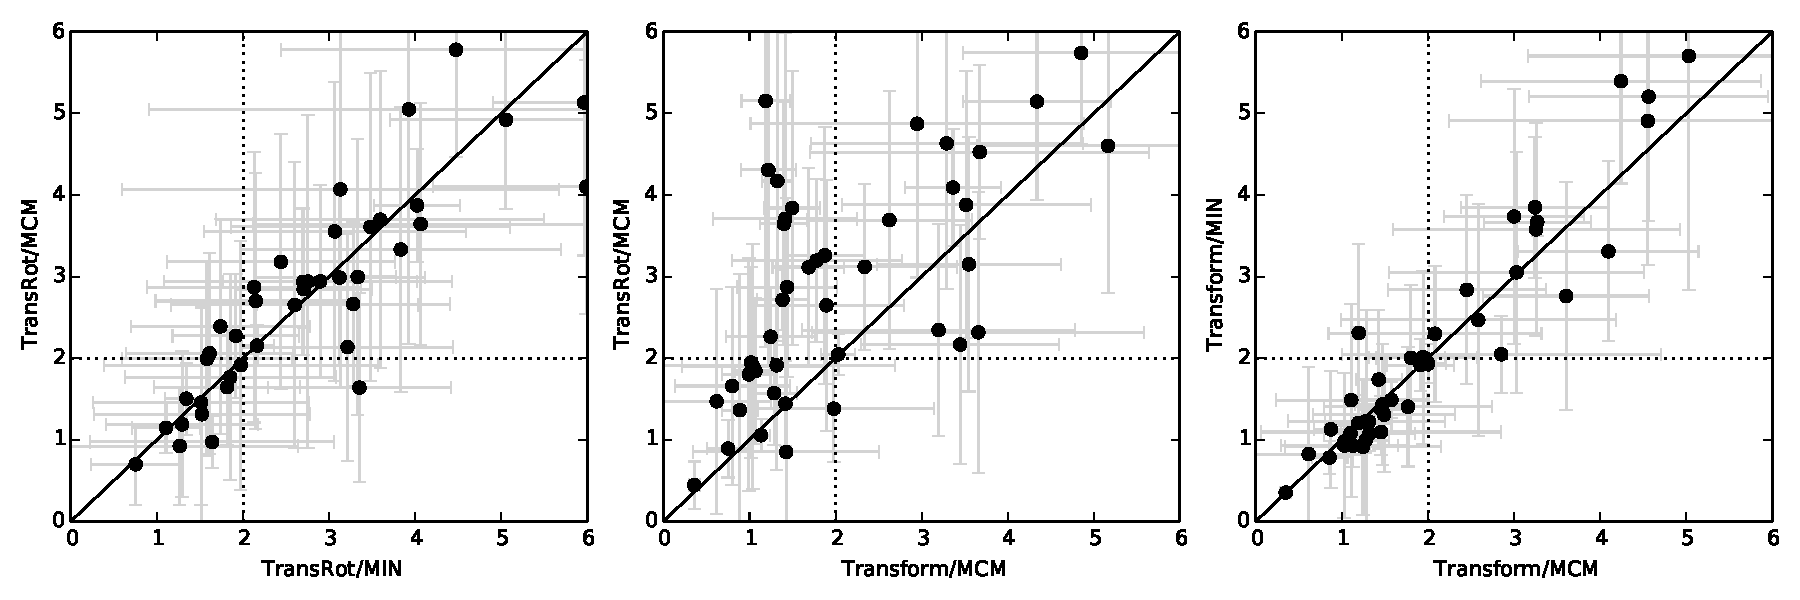
\includegraphics[width=4in]{figures/lowres/rmsd_vs_rmsd_relax.pdf}
\caption{
RMSD vs RMSD plots comparing the performance of various docking protocols when docking ligands into relaxed structures.
20 samples of 150 models were collected, and the average of the RMSD of the lowest scoring model is plotted for each protein-ligand system.
The standard deviation of these 20 samples is shown with error bars. Dotted lines indicate the 2.0 \AA\ RMSD cutoff used to classify correct vs incorrect poses. 
}
\label{fig:rmsd_vs_rmsd}
\end{figure}

\subsection{Examination of the successes and failures of RosettaLigand illustrates the impact of the \textsc{Transform} algorithm}
Figure \ref{fig:specific_comparison} illustrates several examples of the successes and failures of RosettaLigand.
Figure \ref{fig:specific_comparison}A is an example of a case in which both the \textsc{Transform} and \textsc{TransRot} based algorithms are capable of successfully docking the ligand.
In both cases, the RMSD between the native ligand position and the predicted ligand position is less than 0.5 \AA.  This example represents a ?best case scenario? for RosettaLigand.
The ligand is relatively small, and is deeply buried in the protein, making close contacts with protein-side-chains on almost all sides.
This drastically reduces the possible sampling space available during both initial placement and minimization.
Figure \ref{fig:specific_comparison}B is an example which demonstrates a failure of the \textsc{TransRot} algorithm which is corrected by the \textsc{Transform} algorithm.
The lowest scoring model generated by the \textsc{TransRot} based protocol is flipped 180\textdegree\ about the long axis and less tightly packed in the binding site compared to the lowest scoring model generated by the \textsc{Transform} protocol.
Notably, the final score of the \textsc{TransRot} generated model is significantly higher than the score of the \textsc{Transform} generated model (-7.71 REU vs -14.57 REU). 
This suggests that the failure of the \textsc{TransRot} based protocol is a result of a failure to sample the correct conformation.
Because the \textsc{Transform} mover is able to sample translation and rotation simultaneously, more time will be spent sampling reasonable docking positions of long and narrow ligands like the one in this case, which increases the probability of the initial placement algorithm identifying a near-correct binding position for the refinement algorithm to refine and score.
There are some cases in which neither protocol is able to predict the binding pose.
Figure \ref{fig:specific_comparison}C is one such example.  In this case, the problem is most likely a failure of the Rosetta scoring function used in the Refinement stage.
In the native crystal structure, the ligand is involved in pi-stacking interactions with two phenylalanine residues in the protein.
The Rosetta energy function is currently unable to directly model pi-stacking interactions, and thus will not properly score a native-like conformation. 

\begin{figure}
%figure 6 in orginal paper
\centering
\includegraphics[width=4in]{figures/lowres/specific_comparison.pdf}
\caption{
Comparison of specific successes and failures between the RosettaLigand protocols.
Native structures are in grey, lowest scoring models generated by the \textsc{Transform}/MIN protocol in blue, and lowest scoring models generated by \textsc{TransRot}/MIN in pink.
A) A case in which both tested protocols successfully recovers the native binding position.
B) A case in which \textsc{Transform}/MIN successfully recovers the native binding position, while \textsc{TransRot}/MIN fails.
C) A case in which both protocols fail to recover the native binding position. 
}
\label{fig:specific_comparison}
\end{figure}

\subsection{The \textsc{Transform} algorithm improves performance by improving sampling}
The improvements yielded by the introduction of the \textsc{Transform} algorithm are likely a result of the types of moves performed during sampling.
Because the original \textsc{TransRot} algorithm performs translation and rotation steps separately, it will be difficult to produce a move from the starting position that requires simultaneous translation and rotation.
By simultaneously transforming the ligand in all dimensions, the space of the binding site can be more effectively sampled. 

\subsection{The benefit of the MIN refinement is primarily logistical, but important for vHTS studies}
While Figure \ref{fig:fraction_successful_time} and Figure \ref{fig:fraction_successful_time} indicate that both the MIN and MCM refinement algorithms have a similar impact on sampling performance and average run time, the substantially reduced variability in run time of the MIN refinement algorithm illustrated in Figure \ref{fig:time_per_model} provides a major practical advantage to using MIN rather than MCM for refinement.
When docking a large number of ligands on a computing cluster, a protocol with a predictable run time is highly advantageous as it allows for more efficient utilization of the available resources of the cluster. 
For this reason, while the two refinement methods have similar scientific performance, we recommend using MIN refinement, rather than MCM refinement. 

\subsection{Improving the speed of RosettaLigand increases the number of compounds that can be feasibly screened, enabling vHTS studies}
Given that RosettaLigand is an "Embarrassingly Parallel" application, and thus scales linearly with the amount of available CPU resources, a substantial reduction in required runtime per ligand is extremely valuable.
By reducing the total processing time per ligand from several hours to approximately 15 minutes, it now becomes possible to screen large libraries of compounds.
This development makes the use of RosettaLigand as a virtual High Throughput Screening (vHTS) tool computationally feasible for the first time.

\subsection{It should be possible to further improve ligand docking performance through the addition of scoring information}
The binary scoring grid used in the experiments described above provides a limited amount of information about the protein binding pocket.
A more informative scoring grid could be valuable in further improving the efficiency and performance of RosettaLigand.
Three novel grids based on knowledge based potentials describing shape complementarity and hydrogen bonding information were developed to explore this possibility.
The implementation and benchmarking of these novel grids are described in the attached supplementary information. 
As described in the supplement, these new scoring grids do not have a significant impact on sampling efficiency.
While the incorporation of additional information is potentially very valuable, the uncertainty associated with the position of backbone and side-chain atoms during low resolution docking limits the value of this scoring data.
Research into effective methods of introducing useful scoring data into the initial placement phase is ongoing.
The results described here demonstrate that even in very complex optimization problems such as protein-ligand docking, relatively small changes in sampling and score function evaluation can have a  large impact on performance. 

\section{Methods}
\subsection{Complete docking protocol with high resolution refinement}
\subsubsection{Introduction to protein preparation}
Complete command lines and instructions for the protein preparation are included in the supplemental protocol capture document.

\subsubsection{Description of crystal structure preparation}
The original crystal structures from the CSAR dataset were processed to remove existing water molecules, and hydrogens were added using Rosetta.
The side-chains and protein backbone were left at the crystallographic positions.

\subsubsection{Description of repacked structure preparation}
The crystal structures prepared above were repacked in the absence of the ligand using the Rosetta fixbb application.
The backbone was kept fixed, and all side-chain positions were allowed to repack\citep{Kortemme:2004ia}.

\subsubsection{Description of relaxed structure preparation}
For each of the crystal structures prepared above, 10 relaxed models were produced using the Rosetta relax application.
During the Rosetta relax protocol, cyclic repacking of the side-chains and gradient based minimization of the backbone are used to perform MCM of the entire protein structure.
In this case, all CA atoms were restrained to within 0.3\AA\ of the crystallographic coordinates, to prevent major conformational shifts.
Relaxation was performed in the absence of the ligand.

\subsection{Ligand Conformer preparation}
\subsubsection{Description of ligand conformer generation}

Conformers were generated for each ligand using the BCL::ConformerGeneration application(unpublished).
BCL::ConformerGeneration uses a stochastic fragment assembly approach to conformer generation, utilizing a database of fragment conformations derived from the Cambridge Structural Database. 
A maximum of 100 conformers were generated per ligand, though the actual number of generated conformers varies based on the structure of the ligand and the number of rotatable bonds. The generated conformers were used to produce params files and ligand rotamer libraries using the protocol detailed in the supplementary protocol capture.

%\include{RosettaHTS}
%\chapter{Conclusions and Future Directions}
\label{chap:conclusion}
\section{Summary of Findings}

\subsection{Development of a Novel Energy Function and Benchmarking Method for Protein Design }
The development of of tools for accurate structural biology predictions is an important area of current research.
Tools which can accurately model the effect of mutations on protein stability will make it possible to both explore the basic physical principles that drive protein stability, as well as engineer new proteins and enzymes for pharmaceutical and chemical purposes.
While supercharging \citep{MichaelSLawrence:2007cv,Kurnik:2012dz,Simeonov:2011jf} of protein surfaces has been an effective means of improving the solubility of designed proteins, this technique has and impact on the rate of folding.
Artificially recapitulating the balance between solubility and ability to fold which is seen in natural proteins.
In the service of this goal, chapter \ref{chap:nv_kbp} describes a novel method for designing native-like protein surfaces, as well as a novel quality metric for assessing protein designs.

The new energy function implements a knowledge based potential previously developed by Durham et al. \citep{Durham:2009kt} which was computed based on the propensity of amino acids existing at various degrees of burial in X-ray crystal structures of soluble proteins.
This energy function is effectively an environment potential, which provides an energy bonus to amino acids which are frequently in nature at a given degree of burial within the protein.
In addition to the implementation of this knowledge based potential, the weights of the RosettaDesign energy function were re-optimized to maximize the \ac{PSSM} score of the protein, based on a \ac{PSSM} generated using \ac{BLAST}.
To assess the quality of the proteins designed with the new energy function, two metrics were used.
The first metric was sequence recovery \citep{Kuhlman:2000tc}, the percentage of amino acids which were designed to be identical to the native amino acid.
The second metric, \ac{PSSM} recovery, was originally presented in chapter \ref{chap:nv_kbp}.
\ac{PSSM} recovery is the percentage of amino acids with a favorable \ac{PSSM} score according to a \ac{PSSM} created using \ac{BLAST}.
\ac{PSSM} recovery is advantageous over sequence recovery as a metric of protein design because it measures evolutionarily favorable mutations, rather than simply counting exact amino acid recovery.
Through the combination of this optimization function and the environment based knowledge based potential resulted in protein designs which were more native-like relative to the previously published Rosetta design function.
Specifically, \ac{PSSM} recovery improved from 72\% with the standard energy function to 77.2\% with the optimized energy function.

\subsection{Improvement of the speed and sampling efficiency of RosettaLigand}
While RosettaLigand has been previously successful at ligand docking \citep{Lemmon:2012ku,Combs:2011db,Allison:2013ir}, it is too slow for use in high throughput ligand docking applications.
To address this, chapters \ref{chap:lowres_paper} and \ref{chap:lowres_appendix} describe the development of a grid based Monte Carlo sampling algorithm for initially placing ligands in the protein binding site prior to refinement and a modular scoring system for defining cartesian grid based scoring functions.
The best performing results with the new method were obtained using the new Monte Carlo initial placement algorithm combined with the originally published grid based energy function.
This method resulted in a 10-fold reduction in the number of protein models required to obtain a successful binding pose, as well as a 6 fold reduction in the time necessary to generate a single model.
Additionally, the new RosettaLigand initial placement algorithm results in a significantly increased ability of RosettaLigand to successfully dock ligands into protein systems, and an improved tolerance of backbone and sidechain misplacement.
It is notable that these improvements resulted entirely from improved initial sampling, rather than scoring.
These results highlight the importance of a high quality and efficient sampling in protein-ligand docking, and demonstrate that substantial gains can be made in docking performance through more efficient utilization of existing scoring information.
The results presented in chapter \ref{chap:lowres_paper} make it possible for the first time to efficiently use Rosetta ligand for the structure based virtual screening of large compound libraries on a small academic computing cluster.

\subsection{Development of RosettaHTS: A structure based virtual screening protocol}
The methods developed in chapter \ref{chap:lowres_paper} lead naturally to chapter \ref{chap:rosetta_hts}, which describes the development of a protocol for docking large numbers of small molecules using RosettaLigand and a novel \ac{ANN} based classification model for predicting the activity of these compounds.
To training the \ac{ANN} model, a training data set was constructed using cross-docking so as to be highly diverse in chemical and protein space, as well as balanced in chemical space between active and inactive compounds.
In addition to previously developed Rosetta energy terms, interface quality metrics, and ligand descriptor information, a new set of protein-ligand interface descriptors were developed based on \ac{RDF}s.
Several networks were trained using various combinations of these descriptor sets.
Analysis of the cross-validation performance of the trained networks indicated that the majority of the useful information to the networks was provided by the Rosetta energy term and interface quality metric data.
The cross-validation performance also demonstrated that the networks were well-trained and capable of making more accurate ligand activity classifications than the RosettaLigand interface scores alone. 
Despite the encouraging cross-validation performance of the \ac{ANN} models, screening of the DEKOIS 2.0 benchmark showed that the models were unable to consistently classify active ligands, although significantly fewer protein systems had worse than random performance relative to using the RosettaLigand interface score alone for classification.
Further work is underway to address this issue, and is detailed in section \ref{subsec:hts_further_development}

\section{Future Directions}

\subsection{RosettaLigand method development}

\subsubsection{Scoring function development}
While the RosettaLigand algorithm improvements described in chapter \ref{chap:lowres_paper} are highly encouraging, there is likely further improvements which can be made in both the speed and scientific performance of the software.
One obvious area of further development is in the grid based energy function used by the initial placement algorithm.
The current energy function serves primarily to identify regions of the protein binding site in which atoms placed would result in major clashes with the protein backbone.  
Adding additional information would potentially improve the efficiency with which the Initial placement algorithm can identify high quality binding poses, further reducing the number of binding poses required for a high quality prediction.
The shape complementarity and hydrogen bonding potentials described in chapter \ref{chap:lowres_appendix} represent one attempt to address this problem, but these energy functions did not serve to improve the performance of RosettaLigand.
The likely culprit here is the over-reliance on side-chain positions.
Because the shape complementarity and hydrogen bonding potentials are constructed using all protein atoms, incorrect side-chain positions will result in poor binding position predictions.
Because starting side-chain positions can be assumed to be incorrect if a ligand is being cross-docked, or docked into a comparative model or relaxed structure, any method which relies on side-chain information is likely to be unsuccessful.
To address this problem, research into the development of knowledge based potentials using backbone, C$\alpha$ and C$\beta$ atoms is ongoing.
These potentials are generated using well packed crystal structures with non-covalently bound ligands as input, and encode the propensity of said ligand atoms relative to the protein backbone atoms.
Several methods of accomplishing this are being explored, including the use of purely distance based potentials, 3D potentials utilizing a distance and two angles, and 2D potentials utilizing a distance and one angle.

\subsubsection{Sampling method development}
The Monte Carlo initial placement algorithm described in chapter \ref{chap:lowres_paper} has proven highly useful, but has room for improvement.
The Metropolis Monte Carlo search is performed at a constant Boltzmann temperature.
While a constant temperature search has proven sufficient, a Monte Carlo Simulated Annealing algorithm in which the temperature is initially raised and then slowly lowered could result in faster and more reliable convergence. 
Additionally, the temperature can be dynamically modulated to reach a target acceptance rate.
In this method, the target acceptance rate is gradually lowered over the course of the simulation to cause convergence.
To reach the target acceptance rate, the Boltzmann temperature is modulated continuously.

Pre-computed grid based scoring functions lend themselves well to a variety of sampling methods, some of which may be far more efficient than a monte carlo search.
In particular, if more informative scoring grids can be developed, geometric hashing methods, such as those previously used for CryoEM fitting \citep{Woetzel:2011id} could be of great value.
A geometric hashing algorithm would be capable of identifying potential initial ligand positions far more rapidly than a Monte Carlo search.
Additionally, such an algorithm would make it possible to greatly expand the size of the scoring grid, potentially allowing RosettaLigand to be used to perform binding site detection, rather than requiring that the user provide the initial binding site. 

\subsubsection{Homology model benchmarking}

The results of the benchmarking performed in chapter \ref{chap:lowres_paper} demonstrate that the currently optimal RosettaLigand protocol is capable of docking nearly every protein in the benchmark set used.
For this reason, further development of the sampling and scoring methods described above will likely require the use of a more challenging benchmark, so that the effects of changes to the algorithm can be easily seen. 
To accomplish this, the homology modeling benchmark used by Kaufmann et al. \citep{Kaufmann:2012ck} will be used to for future benchmarking studies.
Preparation of this benchmarking set for use with the modern RosettaLigand protocol is currently underway.

\subsection{RosettaHTS method development}
\label{subsec:hts_further_development}
\subsubsection{Further development of protein-ligand interface descriptors}
The RDF descriptors described in chapter \ref{chap:rosetta_hts} appeared to provide no meaningful information to the ANN models.
Despite this, it is likely that it is possible to develop meaningful fingerprint descriptors for use in these neural networks.
The RDF fingerprint implementation has several parameters which can be potentially optimized to improve performance.
Specifically, the magnitude of the smoothing factor, number of bins in the fingerprint, and maximum fingerprint range are being optimized.
In addition to optimizing the parameters of the RDF fingerprints, several other methods for producing fingerprints can be explored.
The FEATURE framework \citep{Halperin:2008ce} is a method producing fixed length protein environment fingerprints.
This method has been successfully used to identify protein-ligand binding pockets and classify protein binding interactions. 
The FEATURE framework describes the chemical environment surrounding points in space, as a result it can be adapted for use as a ligand interaction descriptor.
Similarly, a 3D autocorrelation function, similar to that implemented in ADRIANA \citep{Code:2011uf} could be valuable as a fingerprinting method.
The FEATURE framework and 3D Autocorrelation methods are less detailed than the \ac{RDF} fingerprints and may result in less noisy and therefore more effective descriptions of the protein-ligand interface.

\subsubsection{Improving neural network generality}
The ANN models trained in chapter \ref{chap:rosetta_hts} improved classification performance beyond the use of the RosettaLigand interface score alone within the scope of protein and ligand chemical space seen in the cross-validation data set.
However, application of these models to a benchmark with chemical space that significantly diverged from the training set resulted in degraded performance, suggesting that the \ac{ANN} models are still limited in their ability to make general predictions.
While the most computationally straightforward means of improving the ability of the network to make general predictions would be to improve the size and scope of the training data set, the lack of available binding affinity and structural data makes this approach infeasible. 
Luckily, several recent innovations in machine learning techniques may provide a method for improving the ability of \ac{ANN}s to make general predictions without massively increasing the size of the training dataset.
\ac{DBN} methods \citep{Hinton:2006dy} have recently been shown useful in the training of networks capable of making general predictions in the fields of image recognition \citep{Le:2013kz,Bengio:2009kb} and speech recognition \citep{Heigold:2013us}.
These \ac{DBN}s consist of many layers of hidden neurons, with each layer consisting of hundreds or thousands of neurons.
The large number of hidden neurons makes these networks capable of modeling more complex, indirect relationships than traditional \ac{ANN}s are capable of.
Furthermore, these networks can be "pre-trained" using unlabeled data, and can identify features in the descriptor space in an unsupervised fashion, then fine-tuned using a smaller subset of data with known outputs.
In principle, this approach could be used to produce a more general model of ligand binding without obtaining more labelled experimental data.
In a \ac{DBN} based protocol, the network would be pre-trained using the combined set of known training and unknown screening data without any labels attached.
This would result in a pre-trained network with "knowledge" of the full chemical space to which the network will be applied.
This network will then be fine-tuned using the known training data, and then applied to predict the activity of the unknown screening data.

There are several potential pitfalls and complications regarding this approach.
First, the \ac{BCL} machine learning tools do not currently implement a \ac{DBN} in a means that would be amenable to this training method.
Theano \citep{Bergstra:2010tc} is a Python library designed to facilitate the implementation of complex machine learning systems.
Theano will be used to rapidly prototype a \ac{DBN} capable of using the previously implemented RosettaLigand descriptors.
The second complication relates to the nature of the descriptors available for protein-ligand binding activity prediction.
The majority of research in \ac{DBN} pattern recognition has focused on machine vision and audio recognition problems.
For this class of problems, each descriptor encodes information of the same kind.
For example, in the case of an image recognition problem, each descriptor represents the intensity of a pixel at a given point in space.
Different descriptors refer to different regions of space, but each descriptor is otherwise encoding the same information.
Furthermore, nearby descriptors encode similar, or in some cases, effectively identical information.
An image of a cat, for example, with two adjacent pixels swapped, is still an image of a cat.
The descriptor information provided as a result of ligand docking simulations is very different in that adjacent scalar descriptors can represent radically different types of information.
Additionally, the set of descriptors currently used by RosettaHTS is significantly smaller than that used with traditional machine vision and audio recognition problems.
From the existing literature in the field, it is not clear whether the presence of a large number of descriptors encoding homologous types of information is critical to obtain the classification performance exhibited by \ac{DBN}s in other fields.
As a result, while \ac{DBN}s show promise in other fields, it is difficult to predict whether this type of network will be as applicable to the problem posed by RosettaHTS.
Luckily, it should be possible to determine whether this approach will be valuable relatively quickly.
%\chapter{Appendix: Rosetta HTS ligand pre-processing}
\label{chap:hts_preprocess}
\section{Background}

\ac{vHTS} in Rosetta poses a number of unique challenges.
Large numbers of ligands must be prepared and managed.
If multiple protein systems are being screened, the appropriate ligands must be matched with the appropriate proteins. 
Additionally, because Rosetta currently stores ligand information after it is required, the memory requirements of the protocol increase as more ligands are screened.
The most straight forward way to address this is to limit the number of ligands screened in each process.

This protocol describes a series of scripts that can be used to rapidly prepare a set of proteins and ligand for virtual high throughput screening.

All scripts referenced can be found in \texttt{tools/hts\_tools}

\section{Prerequisites}

This protocol requires the following:

\begin{itemize}
\item Python
\item BioPython
\item The most recent weekly release of Rosetta.
\item A directory containing conformations of all the proteins in your screening study.
\item An \ac{SDF} containing all the conformers of all the ligands you want to dock. All conformers of the same ligand must have the same name.
	\begin{itemize}
	\item All conformers of all ligands must have 3D coordinates and hydrogens.
	You will receive no errors or warnings if you provide ligands with 2D coordinates or without hydrogens, but you will get very poor ligand docking results.
	\end{itemize}
\end{itemize}

\section{Protocol}

\subsection{Split ligands}

The first step of the protocol is to split the ligand file.
\texttt{sdf\_split\_organize.py} will accomplish this task. 
It takes as input a single \ac{SDF} file, and will split that file into multiple files, each file containing all the conformers for one ligand.
Different ligands must have different names in the \ac{SDF} records, and all conformers for one ligand must have the same name. 
Output filenames are based on the sha1 hash of the input filename, and are placed in a directory hashed structure.
Thus, a ligand with the name ``Written by BCL::WriteToMDL,CHEMBL29197''
will be placed in the path\\
\texttt{/41/412d1d751ff3d83acf0734a2c870faaa77c28c6c.mol}.

The script will also output a list file in the following format:

\begin{verbatim}
ligand_id,filename
string,string
ligand_1,path/to/ligand1
ligand_2,path/to/ligand2
\end{verbatim}

The list file is a mapping of protein names to \ac{SDF} file paths.

Many filesystems perform poorly if large numbers of files are stored in the same directory. 
The hashed directory structure is a method for splitting the generated ligand files across 256 roughly evenly sized subdirectories, improving filesystem performance.

The script is run as follows:

\begin{verbatim}
sdf_split_organize.py input.sdf output_dir/ file_list.csv
\end{verbatim}

\subsection{Create ``project database''}

The ligand preparation pipeline uses an sqlite3 database for organization during the pipeline.
The database keeps track of ligand metadata and the locations of ligand files.
The project database is created using the following command:

\begin{verbatim}
setup_screening_project.py file_list.csv output.db3 
\end{verbatim}

\subsection{Append binding information to project database}

The next step is to create a binding data file. The binding data file should be in the following format:

\begin{verbatim}
ligand_id,tag,value
string,string,float
ligand_1,foo,1.5
ligand_2,bar,-3.7
\end{verbatim}

The columns are defined as follows:

\begin{enumerate}
\def\labelenumi{\arabic{enumi}.}
\item \textbf{ligand\_id} --- ligand\_id is the name of the ligand, which must match the ligand\_id in the file\_list.csv file created by \texttt{sdf\_split\_organize.py}.
\item \textbf{tag} --- The name of the protein the ligand should be docked into. If a ligand should be docked into multiple proteins, it should have multiple entries in the binding data file.
  Note that this protocol makes a distinction between protein name, and file name.
  If you have 4 files: \texttt{foo\_0001.pdb}, \texttt{foo\_0002.pdb}, \texttt{bar\_0001.pdb}, and \texttt{bar\_0002.pdb}, then you have two proteins with the names foo and bar.
  The scripts expect that the protein \ac{PDB} files begin with the protein name.
\item \textbf{value} --- The activity of the ligand. If you are doing a benchmarking study and know the activity of your ligand, you should enter it here.
  If you are not doing a benchmarking study, or if ligand activity is not relevant to your study, value can be set to 1.0 (or anything else). 
  This field is currently only used in a few specific Rosetta protocols that are in the experimental stages, and is typically ignored, so it is safe to set arbitrarily in almost every case.
  Regardless, the scripts require that you provide some value.
\end{enumerate}

Once you have created this file, you can insert it into the project
database with the following command:

\begin{verbatim}
add_activity_tags_to_database.py database.db3 tag_file.csv
\end{verbatim}

\subsection{Generate params files}

The next step is to generate params files. \texttt{make\_params.py} is a script which wraps around\\
\texttt{molfile\_to\_params.py} and generates params files in an automated fashion.
params files will be given random names that do not conflict with existing Rosetta residue names (no ligands will be named ALA, for example).
This script routinely results in warnings from \texttt{molfile\_to\_params.py}, these warnings are not cause for concern. 
Occasionally, \texttt{molfile\_to\_params.py} is unable to properly process an \ac{SDF} file, if this happens, the ligand will be skipped. 
In order to run \texttt{make\_params.py} you need to specify the path to a copy of \texttt{molfile\_to\_params.py}, as well as the path to the Rosetta database.

\texttt{make\_params.py} should be run like this:

\singlespace
\begin{verbatim}
make_params.py -j 4 \
--database path/to/Rosetta/main/database \
--path_to_params path/to/molfile_to_params.py \
database.db3 output_dir/
\end{verbatim}
\doublespace

In the command line above, the \texttt{-j} option indicates the number of \ac{CPU} cores which should be used when generating params files.
If you are using a multiple core machine, setting \texttt{-j} equal to the number of available cpu cores.

The script will create a directory \texttt{params/} containing all params files, \ac{PDB} files and conformer files.

\subsection{Create job files}

Because of the memory usage limitations of Rosetta, it is necessary to split the screen up into multiple jobs. 
The optimal size of each job will depend on the following factors:

\begin{itemize}
\item The amount of memory available per \ac{CPU}
\item The number of \ac{CPU}s being used
\item The number of atoms in each ligand
\item The number of conformers of each ligand
\item The number of protein residues involved in the binding site.
\end{itemize}

Because of the number of factors that affect RosettaLigand memory usage, it is usually necessary to determine the optimal job size manually.
Jobs should be small enough to fit into available memory.

To make this process easier, the \texttt{make\_evenly\_grouped\_jobs.py} script will attempt to group your protein-ligand docking problem into a set of jobs that are sized as evenly possible. 
The script is run like this:

\singlespace
\begin{verbatim}
make_evenly_grouped_jobs.py --n_chunks=10 \
 --max_per_job=1000 param_dir/ structure_dir/ output_prefix
\end{verbatim}
\doublespace

If the script was run as written above, it would use param files from the directory \texttt{param\_dir/}, and structure files from the directory \texttt{structure\_dir/}.
It would attempt to split the available protein-ligand docking jobs into 10 evenly grouped job files (\texttt{--n\_chunks}).
The script will attempt to keep all the docking jobs involving one protein system in one job file. However, if the number of jobs in a group exceeds 1000,
the jobs involving that protein system will be split across multiple files (\texttt{--max\_per\_job}). 
The script will output the 10 job files with the given prefix, so in the command above, you would get files with names like ``output\_prefix\_01.js''.
The script will output to the screen the total number of jobs in each file. All the numbers should be relatively similar. 
If a job file at the beginning of the list is much larger than the others, it is a sign that you should reduce the value passed to \texttt{--max\_per\_job}. If the sizes of all jobs are larger than you want, increase \texttt{--n\_chunks}.

\subsubsection{Job file specification}

RosettaLigand Job files are \ac{JSON} files which contain the paths to protein and ligand \ac{PDB} files, the names of the protein systems,
and the params files necessary to load the ligand \ac{PDB} files.
An example file is below:

\singlespace
\begin{verbatim}
 "jobs": [
  {
   "proteins": [
    "set2_28_0001.pdb"
   ],
   "ligands": [
    "A9.pdb"
   ],
   "group_name": "set2_28"
  },
  {
   "proteins": [
    "set1_42_0001.pdb"
   ],
   "ligands": [
    "AJ.pdb"
   ],
   "group_name": "set1_42"
  }
 ],
 "params": [
  "A9.params",
  "AJ.params"
 ]
\end{verbatim}
\doublespace

\subsection{Submit jobs}

Once the jobs have been created they can be input into rosetta using the option\\
\texttt{-in:file:screening\_job\_file job\_file.js}.
If this option is being used, \texttt{-s}, \texttt{-l}, \texttt{-list} and \texttt{-in:file:extra\_res\_fa} should not be used.

%\chapter{Appendix: Managing Rosetta datasets with SQL}
\label{chap:sql_appendix}
\section{Introduction}

Screening small molecule libraries with RosettaHTS requires the generation of very large number of models. 
For example, a screen of 250,000 compounds will result in 50,000,000 generated Rosetta models.
Because RosettaHTS only needs the top 1 model generated for each ligand, 99.995\% of this data will not be needed.
To avoid unnecessarily storing data, RosettaHTS stores generated models in a relational database.
Here  the technical details of the database storage framework used by RosettaHTS are described.
This framework was developed collaboratively by myself, Chris Miles at the University of Washington, Matt O'Meara at the University of North Carolina, and Tim Jacobs at the University of North Carolina, all of whom contributed equally to the project. 

\section{Features reporter architecture}

The data storage framework used by RosettaHTS is a subset of a statistical analysis framework within Rosetta called the Features Reporter.
The Features Reporter framework consists of an \ac{ORM} that allows \ac{SQL} schema definitions, queries and insertion statements to be composed in C++, and a reporting system used for computing statistical data and storing it in the database.
The \ac{ORM} was developed using CppDB(http://cppcms.com/sql/cppdb/) \ac{SQL} library, which allows the features reporter to work with SQLite, MySQL and Postgres database backends.
As all 3 of these back ends have different caveats, behaviors and syntax idioms, the \ac{ORM} is responsible for constructing the appropriate MySQL command and sending it to the server.

In addition to allowing for the transparent support of multiple Database Backends, the \ac{ORM} system makes it possible for a C++ programmer to easily define new \ac{SQL} objects without being familiar with \ac{SQL} syntax. 
For example, the C++ code reproduced below defines an \ac{SQL} table containing structure ID, residue number, 3 letter residue name, and residue type fields, then generate the appropriate \ac{SQL} syntax to create this table, and execute the \ac{SQL} command on the database server.

\singlespace
\begin{Verbatim}
Column struct_id("struct_id", new DbBigInt(), false);
Column resNum("resNum", new DbInteger(), false);
Column name3("name3", new DbText(), false);
Column res_type("res_type", new DbText(), false);

utility::vector1<Column> residues_pkey_cols;
residues_pkey_cols.push_back(struct_id);
residues_pkey_cols.push_back(resNum);

Schema residues("residues", PrimaryKey(residues_pkey_cols));
residues.add_column(struct_id);
residues.add_column(resNum);
residues.add_column(name3);
residues.add_column(res_type);
residues.add_foreign_key(
  ForeignKey(struct_id, "structures", "struct_id", true));

residues.write(db_session);
\end{Verbatim}
\doublespace

This model of database interaction allows multiple database systems to be supported with a single code base, which is critical given the diversity of hardware and software operated by Rosetta users.
Additionally, it allows support to be added for additional database systems without any change to the code defining feature tables. 

The Features Reporter has been previously described in the literature \citep{LeaverFay:2013fn} as a method for collecting and analyzing statistics from large numbers of Rosetta models.  
In the sections below we will describe the specific application and usage of this framework for the storage and retrieval of protein models in a high throughput screening environment. 

\section{Pose storage schema}

RosettaHTS uses a subset of the Features Reporter system to store and retrieve protein structure information from the database.
In the most simple case, it would be possible to store only the atom and residue names, chain information, and cartesian coordinates for each atom, and effectively replicate the information present in a \ac{PDB} file.
However, storing this limited subset of information requires that Rosetta rebuild the internal data-structures representing the protein structure every time the pose is loaded, as is done when taking input from a \ac{PDB} file.
While this is normally acceptable, in rare cases, there are multiple correct configurations that these data structures can take on, and thus, recomputing them can result in a slightly different input model, and numeric inconsistencies in scoring across multiple loads of the structure.
While these  numeric inconsistencies do not typically lead to scientific inconsistencies, their presence can complicate data analysis.

In order to rectify this problem, the RosettaHTS pose storage schema stores not only the information reflected in the protein \ac{PDB} file, but also all of the derived data created by Rosetta.
The storage of this information makes it possible to precisely store and recover the protein structure as it is internally represented by Rosetta.
The Pose storage schema is illustrated in Figure \ref{fig:pose_schema}.  Each block in the figure represents an \ac{SQL} table storing a subset of 
of the information needed to reconstruct the pose.
Connections between the blocks indicate "Relationships" between the tables.  Connecting the tables with relationships makes it possible to link data elements that related to each other, while simultaneously allowing for Pose data to be queried efficiently.

\begin{figure}
%figure 2 in orginal paper
\centering
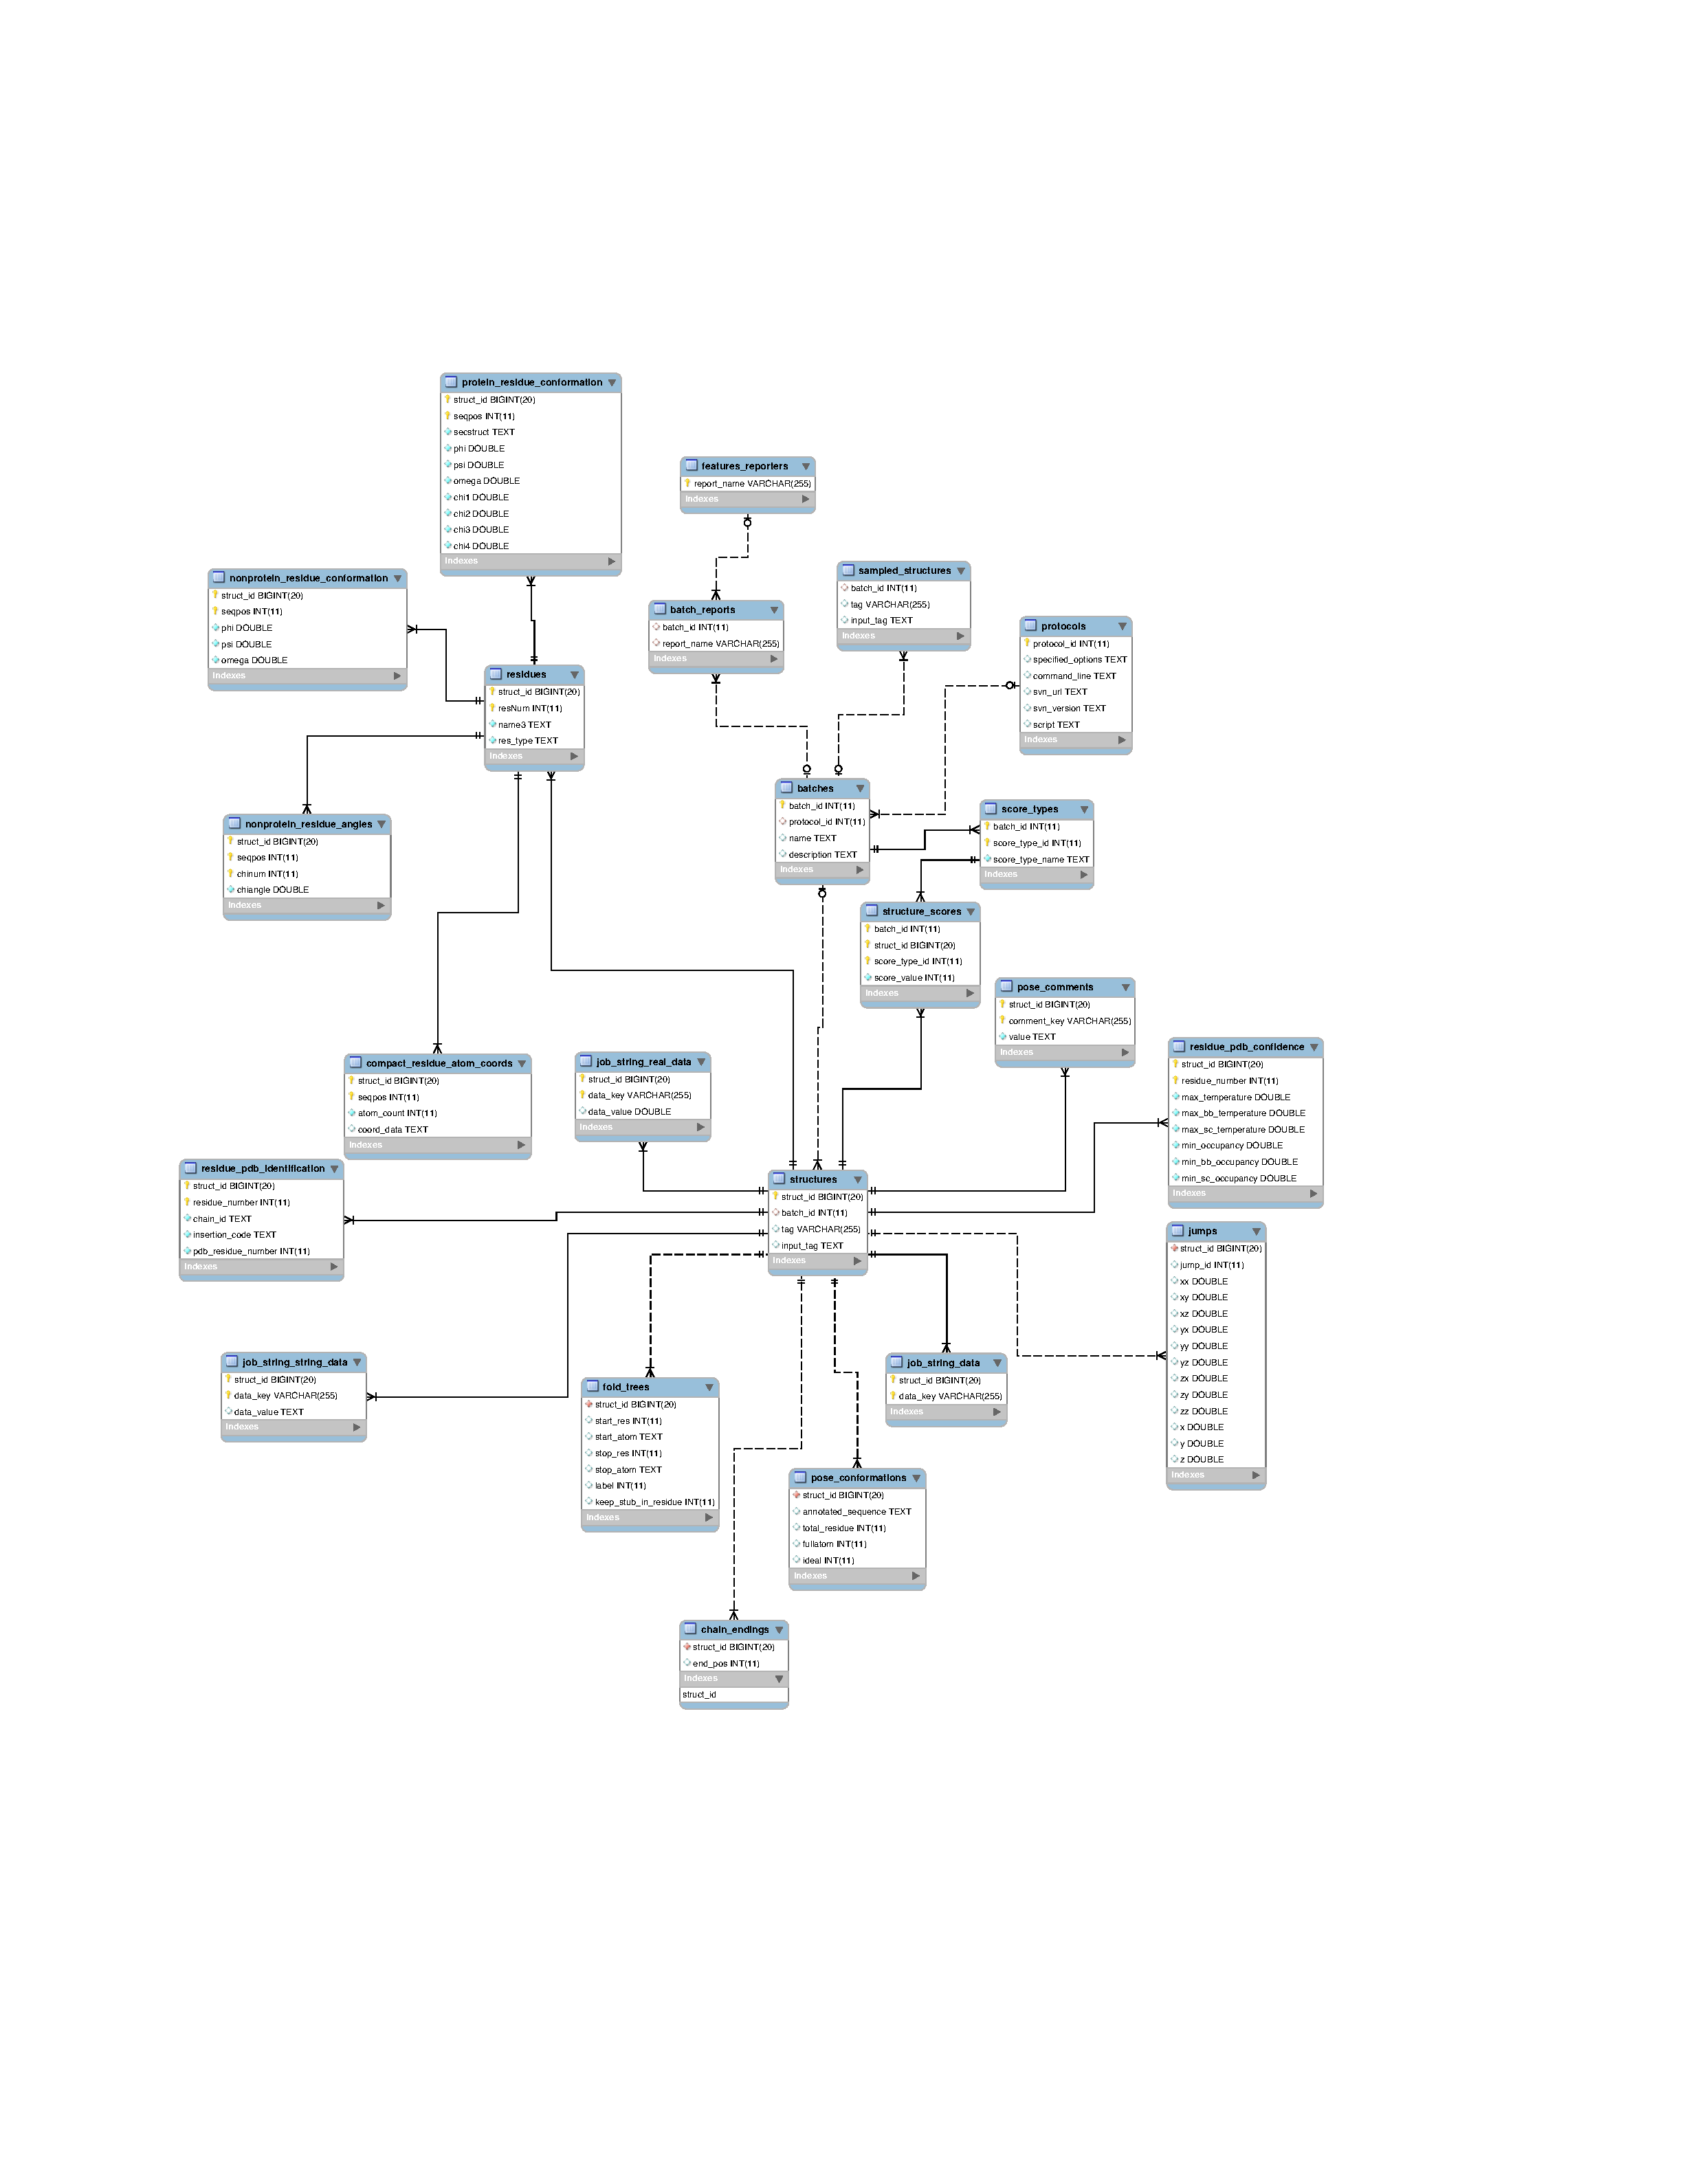
\includegraphics[width=6in]{figures/mysql/mysql_model.pdf}
\caption{
A schematic representation of the information stored by the RosettaHTS pose schema
}
\label{fig:pose_schema}
\end{figure}

A critical component of the design of a relational database schema is a means of uniquely identifying models.
In this case, uniqueness from the point of view of the database has a different meaning than biochemical uniqueness.
If Rosetta is run twice with the same protocol and produces two absolutely identical output models, those models should be stored separately in the database and given unique identifiers, even though they contain the same information. 
Additionally, given a specific stored Pose, it should be possible to identify which execution of the Rosetta application resulted in that Pose, and at what point in the overall protocol the Pose (or other statistical data) was generated. 
To accomplish this, the identification of structures is handled with a three tiered structure.
The top tier is the "Protocol" level.
A new Protocol is generated every time a Rosetta process outputs to a database.
Each protocol has a unique number identifying it which is assigned by the database server.
The Protocol stores the version of Rosetta that was used, as well as the command line options and XML script specified by the user.
Each Protocol can generate one or more "Batch" which is the second level of the identification system.
A Batch is generated every time a Protocol outputs structural data. If RosettaHTS is only outputting completed protein models, only one batch exists per protocol.
If the Features Reporter is also being used in the middle of the protocol to generate extra statistics, additional batches will be generated. 
Each Batch has a unique number identifying it, and references the protocol that was responsible for creating it.
The last tier in the identification system is the "Structure".
A new structure is generated every time Rosetta produces a model.
Each structure has a unique number identifying it, and references the batch that resulted in the creation of that structure.
Additionally, each structure record has a human readable "tag" describing its output, and references the input structure that was used as a basis for the model. 
In this way, the batch, protocol and structure tables can be joined by their related IDs such that, given a structure stored in the database, one can determine precisely what Rosetta command was used to generate that structure, and at what point in the Rosetta protocol the structure was generated. 

The Structure ID described above is used as the central unique identifier, and all the information associated with an individual model is related using this ID.

The RosettaHTS database IO schema stores the following information:

\begin{itemize}
	\item Text and numeric comment data that some Rosetta components insert in a pose for scoring and tagging purposes during the protocol.
	\item The range of B-factors for atoms in each residue.
	\item The "Jumps" in the structure.  Jumps are data structures which represent the spatial relationship between protein chains as a Rotation and Translation matrix.
	\item The sequence associated with the structure, annotated with the identity of any non-canonical, modified or ligand residues.
	\item The ending position of each chain.
	\item The "Fold Tree" defining the structure.  The Fold tree is a data structure used by Rosetta to describe how different parts of the protein are related in space.  Fold Trees can be configured to make it possible to rapidly perturb large parts of the protein as a rigid body.  DiMaio et al. \citep{DiMaio:2011cu} provides an example of a fold tree manipulation in practice.
	\item The Chain ID, insertion code, and residue number present in the original PDB file
	\item The values of each energy term in the score function when the structure was last scored.
	\item The cartesian coordinates of each atom.
	\item The chi angles of each canonical amino acid.
	\item The rotation angles of each non-canonical amino acid or non-protein molecule.
\end{itemize}

In addition to providing infrastructure for outputting Rosetta models, the RosettaHTS pose IO schema provides infrastructure for using this data as input into Rosetta.
Both output to and input from the database is handled by the Rosetta job distribution system.
This means that any Rosetta application can use a database as a data storage mechanism, without any additional programming on the part of the developer of the application.
Furthermore, because the same database can be used for both output and input simultaneously, a Rosetta modeling protocol that relies on different applications being used in different stages can use the database for data management at each stage.

\section{Database Filters}

Historically, Rosetta applications have considered each model independently of each model.
This is primarily an engineering decision.
If each model is considered independently, it means that only the current structure needs to be stored in memory, reducing system resource requirements. 
Additionally, if each model is considered independently, the design of Rosetta is simpler, as it each module of the code does not need to consider the accumulation of state between jobs.
However, while this decision was critical to making Rosetta a maintainable piece of software, it has severely limited the ability to perform filtering and output of models. 
Specifically, filters could historically be created only based on single protein metrics.
A filter could, for example, output models with a score lower than a certain fixed cutoff, or that had a degree of packing better than a cutoff.
However, in the case of protein-ligand docking, we are unable to set fixed score cutoffs, as the range of scores seen will vary from ligand to ligand.
The preferred means of filtering ligand models is to accept the lowest scoring model generated for each protein-ligand pair.
This type of filter cannot be created with the traditional Rosetta filter system, requiring that all models be output, and filtered after the fact.
The RosettaHTS docking protocol requires that 200 models be generated per protein-ligand pair. 
Given that each compressed model requires approximately 90 kilobytes of storage space, the total requirement per protein-ligand pair is roughly 18 megabytes.
Thus, a 250,000 compound screen would require about 4.5 terabytes of compressed storage space. 
The infrastructure required to store and analyze a dataset of this size outstrips the abilities of most research groups, and the storage of the complete dataset is particularly senseless as nearly all of it will be deleted after the initial round of filtering. 

The Database Filter system leverages the properties of the \ac{SQL} database system to make it possible for the first time to create Rosetta filters which take into account the context of previously generated models.
\ac{SQL} is designed to conduct rapid queries of stored data, and as these queries are conducted by the database engine itself, rather than Rosetta, the operation of the filter does not require that state be kept between Rosetta jobs and does not result in additional memory requirements.

A Rosetta Database Filter can have 3 possible outcomes:  The current model is not output, the current model is output, or the current model replaces an existing model.
To accomplish this the Database Filter conducts a query of the existing structures in the database  to identify if the current model is suitable to be output, and to identify the model that it will replace if necessary. 
Currently, filters exist to filter models by the top percent or top count by score.
The creation of additional filters can be accomplished by the implementation of a new DatabaseFilter class with a single method.
While the current usage for filtering by score percentile is relatively simple, the Database Filter framework could hypothetically be used to implement histogram matching filters or other filters requiring deep analysis of the existing dataset.
This would be effectively impossible in the context of the classical Rosetta filtering system, but relatively trivial with a Database Filter.

\section{Performance Considerations and Selection of a Database backends}

Currently, the Rosetta database system supports three different database back ends.
The selection of the appropriate back end is an important consideration, and will depend largely on the way in which the database will be used.

\subsection{SQLite3}
SQLite3 (https://www.sqlite.org/) is the default option for Rosetta database support.
SQLite3 stores the entire database as a single binary file, and the database engine itself is built into Rosetta.
The primary advantage of using SQLite3 is that it requires no additional hardware or software infrastructure, which makes it idea for prototyping a protocol or handling small "one-off" analysis of data.
SQLite3 was designed to be used explicitly with single threaded applications, this means that only a single Rosetta process at a time can write to an SQLite database.
Additionally, SQLite3 produces a very large number of random access operations to the filesystem.
The nature of these operations is such that heavy usage of SQLite3 can severely degenerate the performance of a network file system.
For this reason, we recommend that SQLite3 only be used only with local disks, and preferably with Solid State Drives rather than traditional "Spinning" disks.
Despite these limitations, Rosetta protocols requiring large amounts of memory and complex statistical analysis can be performed very efficiently using SQLite3.
The majority of the data collection and analysis described in Leaver-Fay et al. \citep{LeaverFay:2013fn} was conducted using an SQLite3 database.

\subsection{PostgreSQL and MySQL}

PostgreSQL (http://www.postgresql.org/) and MySQL (http://www.mysql.com/) are freely available server based SQL solutions.
In both cases, an independent server is used, and Rosetta communicates with this server over the network.
The details of the installation and configuration of these systems are beyond the scope of this document, however either piece of software is acceptable for use with RosettaHTS. 
For large scale data operations, PostgreSQL and MySQL have substantial advantages over SQLite3. 
In both cases, many processes can simultaneously write to a single database, and the database server ensures that data is written correctly even for large numbers of concurrent reads and writes.
Additionally, the use of a server based SQL solution offloads the computational and IO complexity involved with reading from and writing to the database to a separate machine than the one running Rosetta.
This separation of work can have a substantial performance benefit.
It is possible to create a Rosetta protocol which produces database requests that outstrip the processing ability of even a reasonably powerful database server.
The precise nature of these limitations will depend on the Rosetta protocol, as well as the specific details not only of the database server software configuration but also the server and network infrastructure being used.
For this reason, we advise empirically determining the performance limitations and requirements of your specific protocol through benchmarking tests prior to large scale screening. 

\section{Storing and retrieving poses from the Rosetta command line}

Rosetta provides a set of command line options for storing and retrieving poses from a database.
These command line options can be used with any Rosetta application other than the "abinitio" application, and will function identically in any protocol.

\subsection{Connecting to a database}

Connecting to a Rosetta database depends on the type of database back end being used.  Regardless of what back end is being used, back end mode and the database name must be specified:

\singlespace
\begin{Verbatim}
-inout:dbms:mode <mode>
-inout:dbms:database_name <db_name>
\end{Verbatim}
\doublespace

where \texttt{<mode>} should be replaced by the database mode (either \texttt{mysql}, \texttt{sqlite} or \texttt{postgres}), and \texttt{<db\_name>} should be replaced by the name of the database file if using sqlite, the schema name if using MySQL, and the database name if using PostgreSQL.

If you are using MySQL or PostgreSQL as a back end, you must specify several additional options connect to the server

\singlespace
\begin{Verbatim}
-inout:dbms:host <host>
-inout:dbms:user <username>
-inout:dbms:password <password>
-inout:dbms:port <port>
\end{Verbatim}
\doublespace

Where \texttt{<host>} is the address of the database server, \texttt{<username>} is the username of a user with permission to read and write from the database, \texttt{<password>} is the password of that user, and \texttt{<port>} is the TCP port that the server is running on. 

Additionally, if you will be running RosettaHTS or any other protocol that results in very large numbers of structures being output to a single database (more than 100,000), the database should be configured to reduce the number of \texttt{INSERT} statements necessary to write a complete model.
This is accomplished by modifying the database storage schema to produce a single record per residue rather than a single record per atom.  This enormously reduces the storage and network bandwidth requirements at the cost of data analyzability, and should be considered a required setting when using RosettaHTS.
Compact schema mode is enabled with the following option:

\singlespace
\begin{Verbatim}
-inout:use_compact_residue_schema true
\end{Verbatim}
\doublespace

\subsection{Writing to database}

Once the database connection options above are specified, Rosetta can be configured to write all output models to the specified database with a single output option:

\singlespace
\begin{Verbatim}
-out:use_database
\end{Verbatim}
\doublespace

If the use of a Database Filter is desired, it should be specified with another option:

\singlespace
\begin{Verbatim}
-out:database_filter <filter_name> <score_term> <value>
\end{Verbatim}
\doublespace

Where \texttt{<filter\_name>} is the name of the database filter to use, \texttt{<score\_term>} is the name of the scoring term to filter by, and \texttt{<value>} is the cutoff value to use. 
At the time of writing, the following filters exist:

\begin{itemize}
	\item \texttt{TopPercentOfEachInput} -- Output models in the top $n\%$ of models for each input structures by specified score.
	The specified cutoff value should be a decimal between 0 and 1. 
	\item \texttt{TopPercentOfAllInputs} -- Output models in the top $n\%$ of models over all input structures by the specified score.
	The specified cutoff value should be a decimal between 0 and 1.
	\item \texttt{TopCountOfEachInput} -- Output the top $n$ models for each input structures by the specified score.
	The specified cutoff value should be an integer.
	\item \texttt{TopCountOfAllInputs} -- Output the top $n$ models over all input structures by the specified score.
	The specified cutoff value should be an integer.
\end{itemize}

\subsection{Reading from a database}

Rosetta can be configured to read input models from the specified database with a single input option:

\singlespace
\begin{Verbatim}
-in:use_database
\end{Verbatim}
\doublespace

Note that both \texttt{-in:use\_database} and \texttt{-out:use\_database} can be used simultaneously.
This is valuable in an interactive protocol, as the results from the current round of iteration can be written to the same database as the results from the previous round. 

It is frequently desirable to read only a subset of structures from a database. 
If the structure IDs of the desired structures are known they can be specified with the following command:

\singlespace
\begin{Verbatim}
-in:dbms:struct_ids <struct_id_list>
\end{Verbatim}
\doublespace

Where \texttt{<struct\_id\_list>} is a space separated list of structure IDs.

If the structure IDs are not known, it is possible to select a subset of the database using an \ac{SQL} select statement:

\singlespace
\begin{Verbatim}
-in:select_structures_from_database <statement>
\end{Verbatim}
\doublespace

where \texttt{<statement>} is an SQL statement that performs a \texttt{SELECT} operation that returns either a struct\_id or tag column from the database.  As a simple example, the statement:

\singlespace
\begin{Verbatim}
SELECT struct_id FROM job_string_real_data 
	WHERE data_key = "total_score" 
	ORDER BY data_value ASC LIMIT 500;
\end{Verbatim}
\doublespace

Would select the structure IDs of the 500 lowest scoring models by total score.
This command line option is potentially dangerous as minimal syntax validation is performed by Rosetta and the specified statement is executed on the \ac{SQL} server.
Make sure only to use this command line option with trusted user input, and do not expose any protocol that uses it as a web server.
%\chapter{Appendix: development and testing of knowledge based scoring functions for RosettaLigand initial placement}
\label{chap:lowres_appendix}
\section{Methods}

\subsection{Shape complementarity scoring grid}

\subsubsection{The need for and challenge of shape complementarity calculation}

Shape complementarity is a useful means of determining whether a ligand is in a well packed, non-clashing conformation relative to the protein binding pocket. 
However, rigorous computation of shape complementarity using a metric like $S_{c}$\citep{Lawrence:1993in}  is too time consuming for our purposes, so a rapid approximation of shape complementarity was developed.

\subsubsection{Description of shape complementarity calculations}

The shape complementarity scoring grid is computed by computing the distance between each square in the grid and the edge of the nearest protein atom, using the standard atom radii included in Rosetta.
The fully populated grid then represents the maximum possible radius that an atom at any given point within the grid can have without resulting in a clash with any other atom.
The effective complementarity of a given ligand atom is then computed by subtracting the radius of that atom from the value in the nearest grid square, resulting in the gap between the ligand atom and the nearest protein atom (Figure \ref{fig:shape_schematic}A). 
To compute an energy based on this gap, a knowledge based potential was used. 
The knowledge based potential was derived by computing the $-log(propensity)$ of a pair of protein and ligand atoms having a gap of a given distance length.
The knowledge based potential was derived using the Top8000 set of high quality crystal structures curated by the Richardson Lab.
The resulting potential is shown in Figure \ref{fig:shape_schematic}C.
The left hand (clashing) side of the potential is computed as a linear slope (indicated in red) when it passes above zero on the x axis, while the left hand side is computed as zero when it reaches the zero axis.
Atoms with large gaps are given scores of zero to avoid unnecessarily penalizing correct poses when a large portion of the ligand is exposed to solvent.
As RosettaLigand uses an implicit solvation model, solvent molecules are not present, and thus not represented in the scoring grid.
\begin{figure}
%figure 1 in original paper
\centering
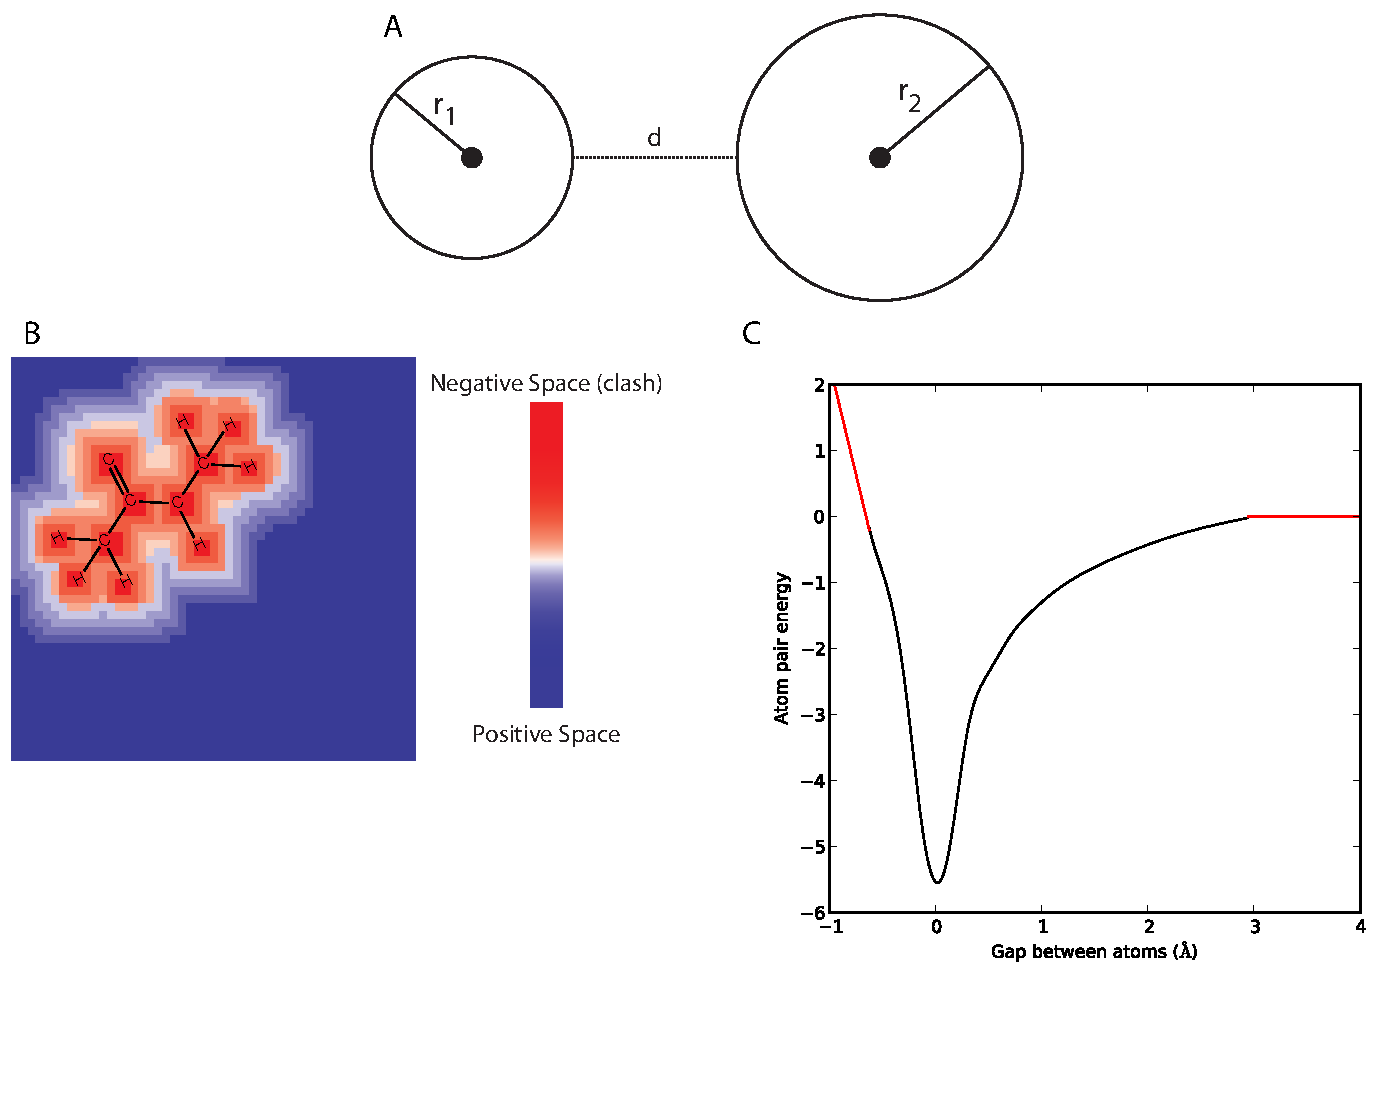
\includegraphics[width=6in]{figures/lowres_appendix/Shape_Complementarity.pdf}
\caption{
A schematic of the Shape Complementarity grid.
A) illustrates the computation of the gap distance between two atoms.
B) Represents the gap distances placed in the scoring grid.
C) Is a plot of the knowledge based potential.
In black is the region directly computed based on the knowledge based potential.
In red are linear functions applied to values beyond the bounds of the potential.
}
\label{fig:shape_schematic}
\end{figure}

\subsection{Hydrogen bond scoring grid}

\subsubsection{Description of hydrogen bond scoring calculations}

Two scoring grids are used to model hydrogen bonding.
As the goal of the initial placement algorithm is to provide a rapid first approximation of ligand position, only distance between hydrogen bond donor and acceptor are taken into account, and angular information is ignored.
A knowledge based potential was created based on the $-log(propensity)$ of a hydrogen bond donor atom being within some distance of a hydrogen bond acceptor atom, using the same Top8000 set of proteins described above (Figure \ref{fig:hbond_schematic}A).
Separate scoring grids are computed for hydrogen bond donors and acceptors. To compute the hydrogen bond donor scoring grid, the distance from each grid square to the nearest hydrogen bond donor is computed, and the score from the knowledge based potential is stored in the grid square (Figure \ref{fig:hbond_schematic}B).
The same process is followed to compute the hydrogen bond acceptor scoring grid.
Hydrogen bond donor atoms are scored based on the value of the nearest grid square in the appropriate scoring grid.  
The combination of the shape complementarity and hydrogen bonding scoring grids are referred to here as the "\ac{KBP}" scoring function. 
\begin{figure}
%figure 2 in original paper
\centering
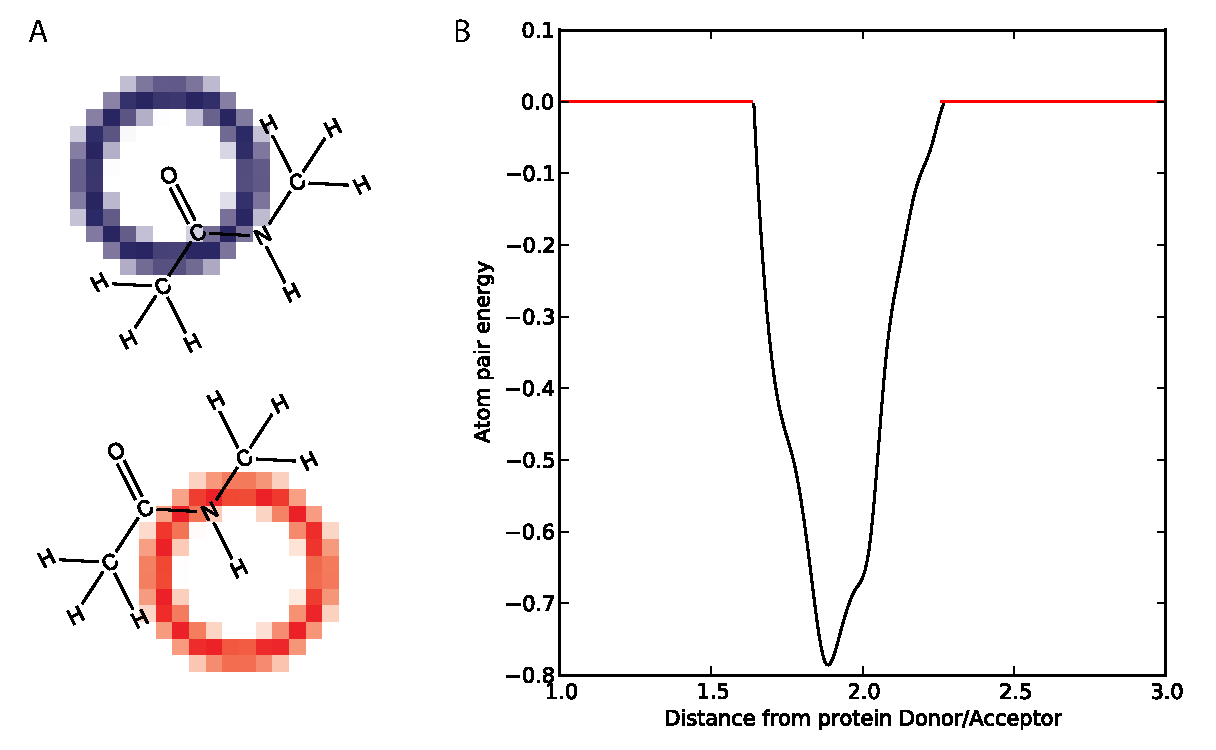
\includegraphics[width=6in]{figures/lowres_appendix/Hydrogen_Bonding.pdf}
\caption{
A schematic of the Hydrogen Bonding grid.
A) a schematic illustrating the placement of scoring information in the hydrogen bonding scoring grids.
B) the knowledge based potential used to populate the scoring grids.
In black is the region directly computed based on the knowledge based potential.  In red are linear functions applied to values beyond the bounds of the potential.
}
\label{fig:hbond_schematic}
\end{figure}

\section{Results and Discussion}

\subsection{The addition of the knowledge based shape complementarity and hydrogen bonding potentials does not improve sampling efficiency}

Figure \ref{fig:frac_time} and Figure \ref{fig:frac_count} compare the effect of the knowledge based potential on docking performance and efficiency.
Figure \ref{fig:frac_time}A and Figure \ref{fig:frac_count}A demonstrate that the new knowledge based potential no significant impact on ligand docking when docking into relaxed models.
Furthermore, when ligands are docked into repacked and relaxed models, the new Knowledge Based Potential demonstrates decreased performance compared to the binary scoring function. 
There are two factors which likely play a role in this decreased performance.
It is notable that as the degree of noise introduced into the protein structure increases, the performance of the \ac{KBP} based scoring grid relative to the Binary scoring grid decreases.
This is effect is most likely caused by the presence of side chain information in the \ac{KBP} based scoring grids.
Because side chain atoms are included, an input model with incorrect side-chains will result in an incorrectly placed energy minimum, and lower quality binding poses. 
The second likely factor is suggested by the shapes of the curves in Figure \ref{fig:frac_count}.
While most ligands are successfully docked within 150 poses, some ligands are exceptionally difficult to dock, and require additional sampling, for this reason, the Transform/Binary/Repack protocol shows a slight increase in success rate after approximately 800 models have been generated.
In contrast, the Transform/\ac{KBP}/Repack protocol does not exhibit the same increase.
This is likely a result of the comparative shapes of the two energy functions.
The Binary energy function is extremely flat, and results in a relatively wide area of space with identical scores.
As a result, a range of ligand poses will be produced during the initial placement stage, as there is not one single energy minimum.
On the other hand, the introduction of a knowledge based potential results in a scoring grid with one or more well defined energy minimums, which will reduce the diversity of allowed initial placements.
If these minima are incorrectly placed as a result of backbone inaccuracies, these incorrect minima will be extensively sampled, reducing overall accuracy of the docking process. 

\begin{figure}
%figure 3 in original paper
\centering
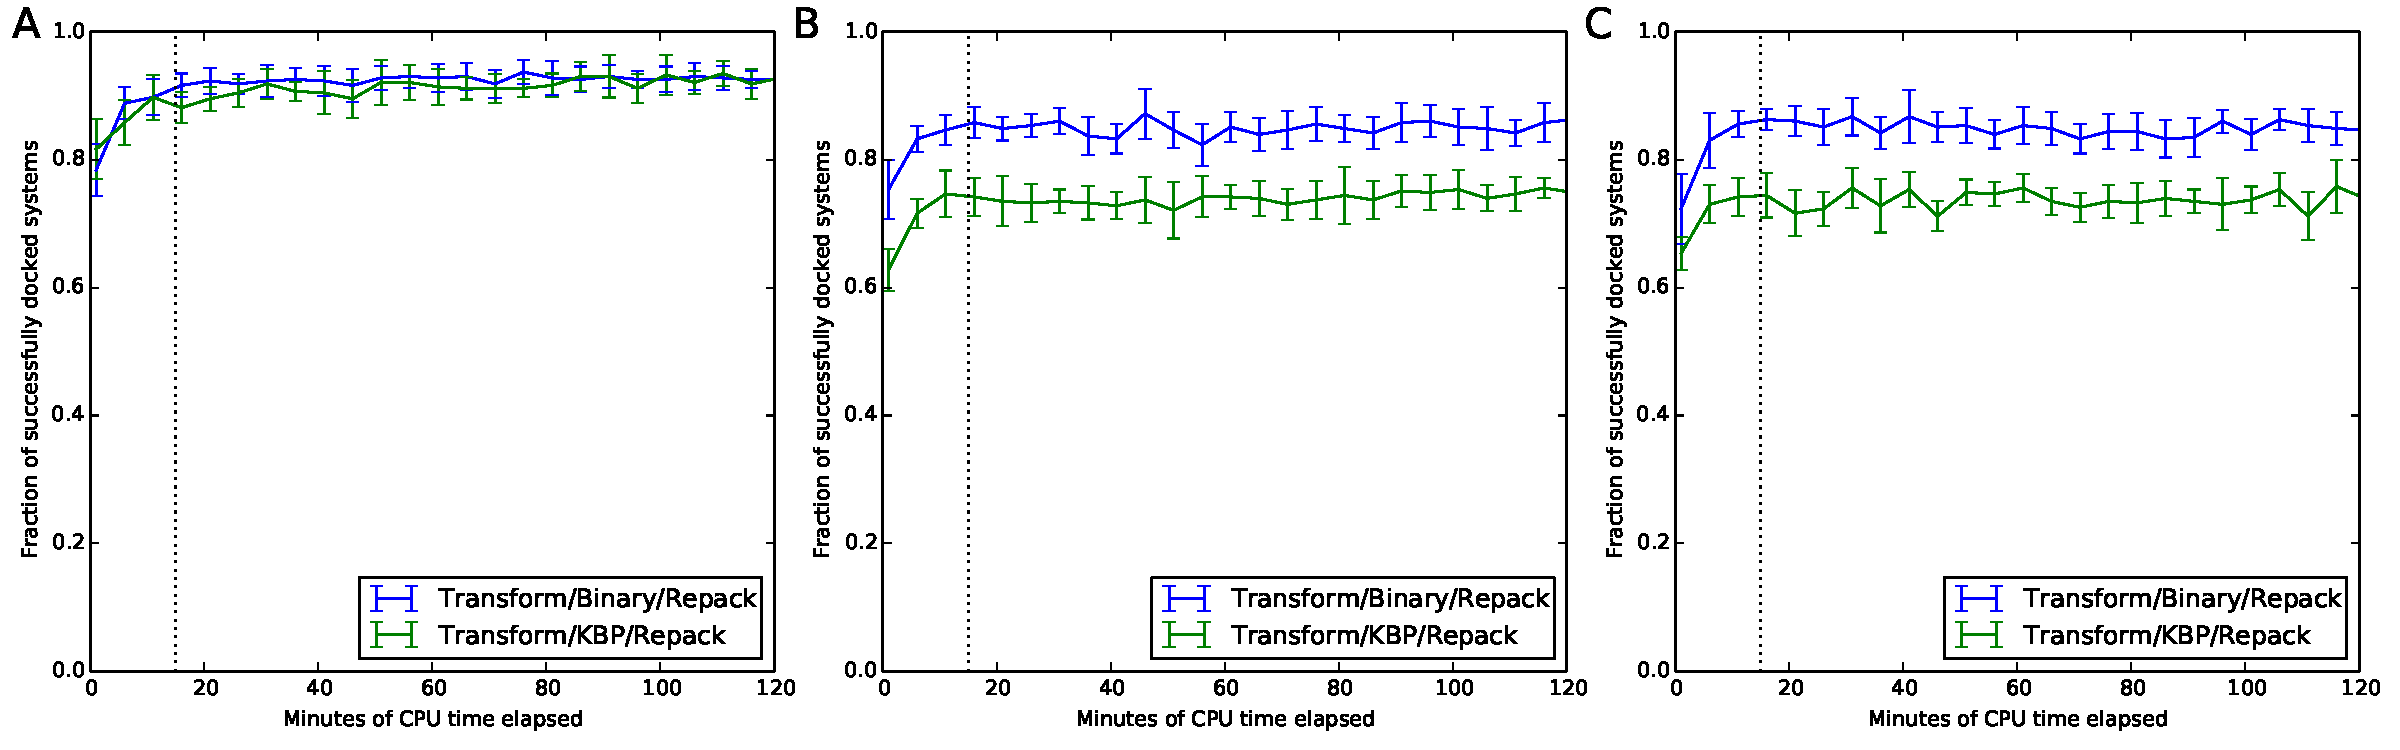
\includegraphics[width=6in]{figures/lowres_appendix/fraction_successful_time_supplement.pdf}
\caption{
The fraction of protein systems in which the lowest scoring model has an \acs{RMSD} < 2.0 \AA\ to the native structure as a function of \acs{CPU} time using the Binary scoring function (Transform/Binary/Repack) and Knowledge based scoring function (Transform/\acs{KBP}/Repack) RosettaLigand docking protocols when docked into A) Crystal structures, B) Repacked crystal structures and C) Relaxed crystal structures. 
A large pool of models were generated, and random subsamples were taken corresponding to time points at 5 minute intervals.
The number of structures included in each time point was based on the average time to generate a model for each algorithm.
20 random samples were taken for each time point, and the means are plotted, with the error bars representing the standard deviation. Docking protocols which make use of the Transform algorithm are reliably converged after approximately 15 minutes (dotted line).  
}
\label{fig:frac_time}
\end{figure}

\begin{figure}
%figure 4 in original paper
\centering
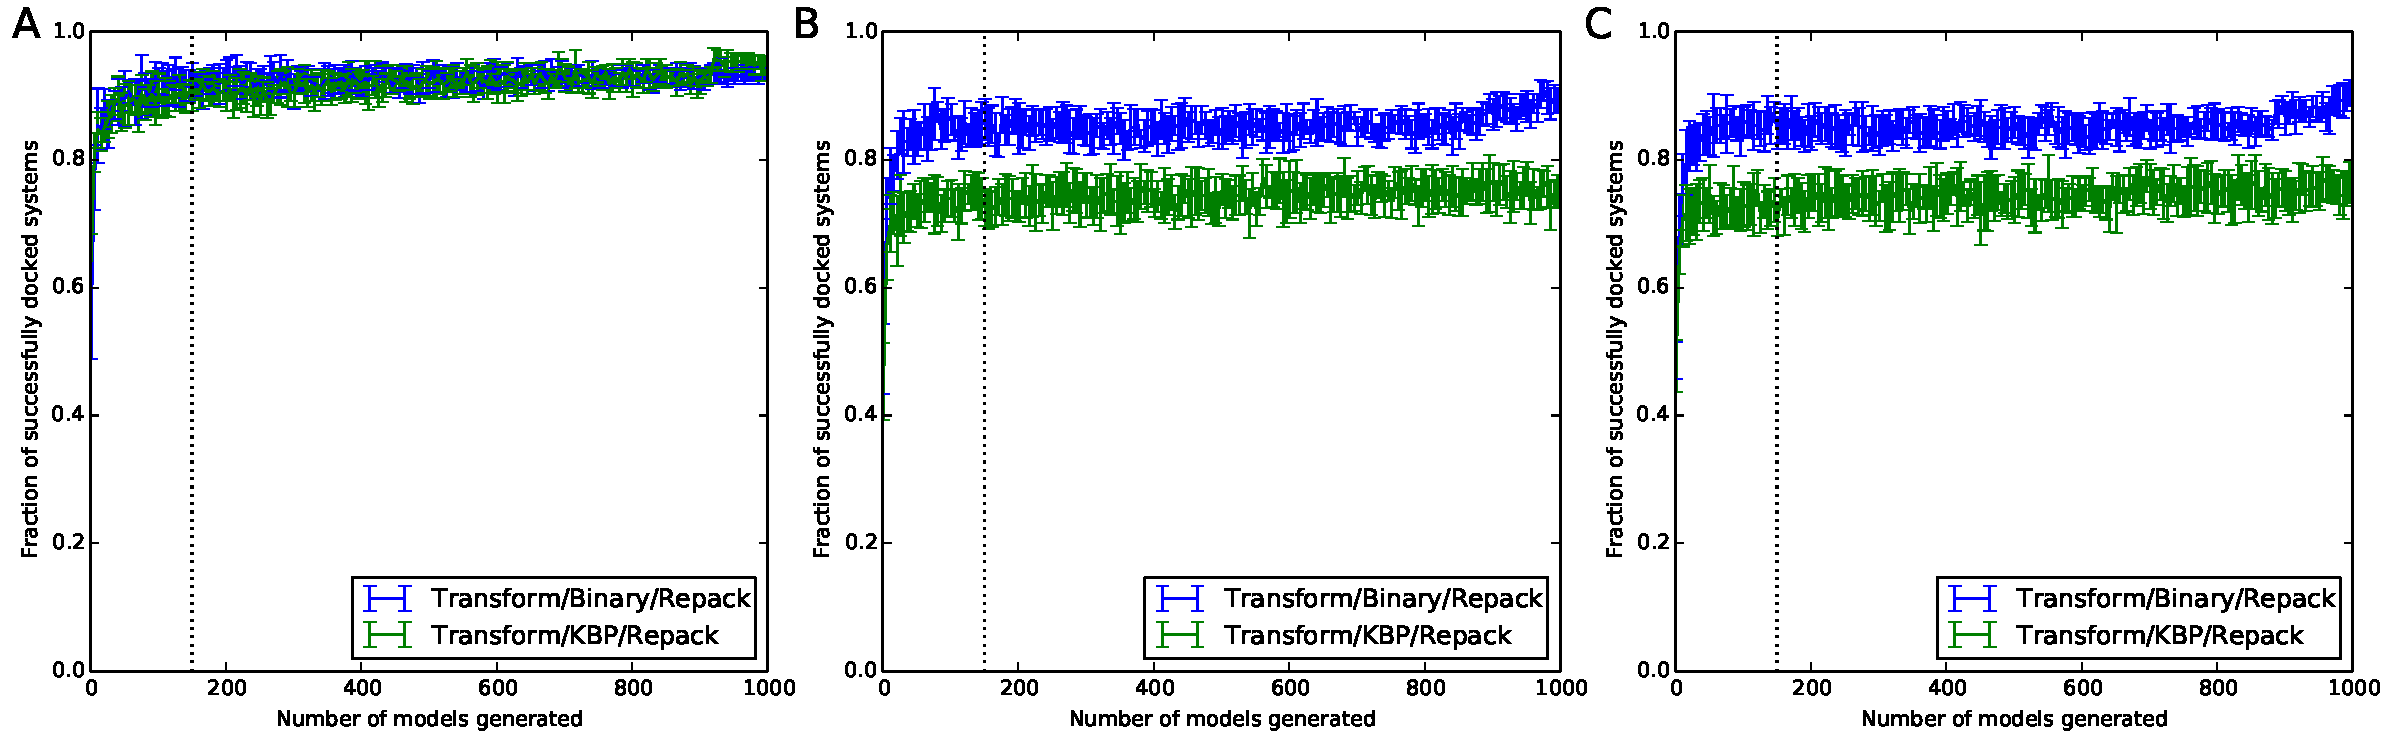
\includegraphics[width=6in]{figures/lowres_appendix/fraction_successful_count_supplement.pdf}
\caption{
The fraction of protein systems in which the lowest scoring model has an \acs{RMSD} < 2.0 \AA\ to the native structure as function of the total number of structures using the Binary scoring function (Transform/Binary/Repack) and Knowledge based scoring function (Transform/\acs{KBP}/Repack) RosettaLigand docking protocols when docked into A) Crystal structures, B) Repacked crystal structures and C) Relaxed crystal structures.
A large pool of models were generated, and random subsamples were taken.
20 random samples were taken for each point, and the means are plotted, with the error bars representing the standard deviation.
Docking protocols which make use of the Transform algorithm are reliably converged after approximately 150 models (dotted line).
}
\label{fig:frac_count}
\end{figure}


%\chapter{Appendix: Protocol capture for chapter \ref{chap:nv_kbp}}

\section{Introduction}

This chapter describes the weight optimization, benchmarking and analysis performed in the work detailed in chapter \ref{chap:nv_kbp}.
Note that the protocol described here was originally performed using Rosetta SVN revision 39040.
In the time since the work described in Chapter \ref{chap:nv_kbp} was performed, the OptE application used here has been drastically rewritten.
As a result, this procedure should not be expected to function correctly (or at all!) when using Rosetta revisions after 39040.

All files referenced in this protocol can be found in the DVD set attached to this thesis. 

\section{Protocol}

\subsection{Weight Optimization}
\label{subsec:nv_weight_opt}
\subsubsection{Overview}
This protocol performs a five way cross validation optimization of the neighbor vector score function using the rosetta optE\_parallel application.
In this setup, 20 rounds of optimization are performed, and the reference energies, fa\_sol and neigh\_vect scoring function are allowed to freely optimize.
The weights are optimized both to maximize PSSM score and to maintain the overall native sequence composition.

\subsubsection{Preparing input structures}
\label{subsubsec:nv_input_prep}
Prior to running OptE, all input crystal structures should be cleaned and relaxed.
To clean the input structures, remove all PDB lines other than ATOM records.
Relaxation is performed using the Rosetta relax application, and the sequence relax protocol.
This protocol can be executed as follows:

\singlespace
\begin{Verbatim}
relax.default.linuxgccrelease -database minirosetta_database/ \
-l input.list -relax:sequence -ex1 -ex2 -ex1aro
\end{Verbatim}
\doublespace

Where input.list contains a list of paths to the input PDB files.
Relaxed files using this method have been provided in Optimization/input\_files/input\_pdbs/

\subsubsection{Generating PSSM files}
PSSM files must additionally be generated for each PDB file prepared in section \ref{subsubsec:nv_input_prep}.
To generate PSSM files, first use the provided script, getFastaFromCoords.pl to create a fasta file based on the relaxed crystal structure.
getFastaFromCoords.py is run as follows:

\singlespace
\begin{Verbatim}
getFastaFromCoords.pl -pdbfile input.pdb > input.pdb.fasta
\end{Verbatim}
\doublespace

The resulting fasta file will then be used as input to BLAST to create a PSSM file.
As the BLAST webserver does not provide PSSM files as output in the proper format, the BLAST application will be used, and is executed as follows:

\singlespace
\begin{Verbatim}
runblast input.pdb.fasta
\end{Verbatim}
\doublespace

The resulting file will produce, among other things, a PSSM file with the file extension .ascii.
This ascii file will be converted to the format required by Rosetta using the provided script convertpssm.py.
The Rosetta expects that the PSSM information be provided as a text file, in which each line of the text file contains the one letter code of a native amino acid, followed by the percentage of observed mutations seen by blast, ordered in alphabetical order by one letter code, and separated by spaces.
This file can be produced using the PSSM generated by blast by running the convertpssm.py script:

\singlespace
\begin{Verbatim}
convertpssm.py -i input.pdb.ascii -o input.fasta.probs
\end{Verbatim}
\doublespace

Note that OptE requires that the file produced by convertpssm.py begin with with the name of the original pdb file, and end with the suffix .ascii.probs.
Additionally, this file must be present in the same directory as the input pdb file.
Thus, a pdb file called "input.pdb" should have a PSSM file of the same name titled input.fasta.probs.
These files are provided in the Optimization/input\_files/input\_pdbs directory.

\subsubsection{Running OptE}
3 sets of optimization were performed using OptE: the optimization of the NV environment KBP, optimization of the reference energies only, and optimization of the reference energies of the final averaged NV environment KBP energy function.
The command files for each optimization are designated by their suffix, and are located in the Optimization/input\_files directory.
"kbp" for files relating to the NV environment KBP optimization, "ref" for files relating to reference energy optimization, and "avg" for files relating to optimization of the averaged energy function.  

In this case, a template PBS file was used, and variables were passed in to this PBS file to start each section of the five way cross validation.
The template file is located in input\_files/optimization\_x.pbs, and the submission commands are located in\\
input\_files/submit\_commands\_x.txt.

See input\_files/flags\_x.txt for the options and comments describing what these options do for each of the 3 optimization experiments performed. 

\subsection{Weight validation and analysis}

\subsubsection{Benchmarking of optimized weights}

The weight sets optimized in section \ref{subsec:nv_weight_opt} were benchmarked using the Rosetta fixbb application.
Fixbb conducts fixed backbone design over the entire protein, using the specified weight set. 
An example command line and flags files can be found in the Benchmark/input\_files directory.
Fixed backbone design was performed on all proteins in both the 100 and 42 protein benchmark sets described in chapter \ref{subsubsec:nv_input_prep}.

\subsubsection{Analysis of benchmarking data}

After the benchmarking designs were performed, the computation of sequence recovery and PSSM recovery was carried out using the script design\_benchmark\_protocol.py, which is provided in the Benchmark/input\_files directory.
This script takes as input a list of paths to native protein structures, and a list of paths to designed protein structures, and outputs a set of CSV files containing the statistics reported in Chapter \ref{chap:nv_kbp}.
The script should be run as:

\singlespace
\begin{Verbatim}
design_benchmark_protocol.py --prefix prefix_file \
native_list.txt designed_list.txt
\end{Verbatim}
\doublespace
%\chapter{Appendix: protocol capture for chapter \ref{chap:lowres_paper}}

\section{Introduction}

This chapter describes the details of the protocol which was described in chapter \ref{chap:lowres_paper}.
The files referenced in this chapter can be found in the DVD attached to the thesis.

\section{Protocol}

\subsection{Conformer Generation}

Conformers can be generated with a number of tools, including MOE and OMEGA.
In this case, the Conformer Generation tool included as part of the BioChemical Library (BCL) suite was used.
The following command was used to generate conformers:
\singlespace
\begin{verbatim}
bcl.exe molecule:ConformerGeneration -conformers \
pdb_refinedsupplemented_lib.sdf.bz2 -ensemble \
rosetta_inputs/ligands/all_ligands.sdf -conformation_comparer \
DihedralBins -temperature 1.0 -max_iterations 1000 \
-top_models 100 -bin_size 30.0 -scheduler PThread 8 \
-add_h -conformers_single_file conformers
\end{verbatim}
\doublespace
You can use any conformer generation tool you have available to you for this step.
Your generated conformers should be output to a single SDF file.
Every conformer must have 3D coordinates and hydrogens added.
Conformers of the same ligand should have the same name in the SDF file.
For convenience, an example conformer file is provided at rosetta\_inputs/ligands/all\_ligands.sdf.

\subsection{Params file generation}

Params files contain the parameterization information for a ligand.
Every  ligand or Residue in a protein structure input into Rosetta must have a corresponding params file.
Rosetta is distributed with a script called molfile\_to\_params.py which generates these files.
However, this script is generally cumbersome for the generation of more than a small handful of ligands.
The protocol below is designed for the preparation of large numbers of ligands.

All the scripts needed for this process are in the tools directory in the Rosetta distribution. 
Each of the scripts below would normally be preceded by Rosetta/tools/hts\_tools, but this directory prefix has been omitted for brevity.

\begin{enumerate}
\def\labelenumi{\arabic{enumi}.}
\item
	\emph{Split ligand files}

	The conformers for all ligands are initially stored in a single SDF file, but molfile\_to\_params.py expects 1 SDF file per ligand.
	sdf\_split\_organize.py accomplishes this task. 
	It takes as input a single sdf file, and will split that file into multiple files, each file containing all the conformers for one ligand.
	Different ligands must have different names in the sdf records, and all conformers for one ligand must have the same name. 
	Output filenames are based on the SHA1 hash of the input filename, and are placed in a directory hashed structure.
	Thus, a ligand with the name "Written by BCL::WriteToMDL,CHEMBL29197" will be placed in the path\\
	 /41/412d1d751ff3d83acf0734a2c870faaa77c28c6c.mol.

	The script will also output a list file in the following format:

	\begin{verbatim}
	ligand_id,filename
	string,string
	ligand_1,path/to/ligand1
	ligand_2,path/to/ligand2
	\end{verbatim}

	The list file is a mapping of protein names to sdf file paths.

	Many filesystems perform poorly if large numbers of files are stored in the same directory.
	The hashed directory structure is a method for splitting the generated ligand files across 256 roughly evenly sized subdirectories, improving filesystem performance.

	The script is run as follows:

	\begin{verbatim}
	sdf_split_organize.py rosetta_inputs/ligands/conformers.sdf \
	split_conformers/ ligand_names.csv
	\end{verbatim}

	Be sure the split\_conformers/ directory exists before running the script.
	Examples of the output of this script are in example\_outputs/ligand\_prep/
\item
	\emph{Create Projet Database}

	The ligand preparation pipeline uses an sqlite3 database for organization during the pipeline.
	The database keeps track of ligand metadata and the locations of ligand files.
	The project database is created using the following command:

	\begin{verbatim}
	setup_screening_project.py ligand_names.csv ligand_db.db3
	\end{verbatim}

  	An example of the project database is in example\_outputs/ligand\_prep
\item
	\emph{Append binding information to project database}

	The next step is to create a binding data file. The binding data file should be in the following format:

	\begin{verbatim}
	ligand_id,tag,value
	string,string,float
	ligand_1,foo,1.5
	ligand_2,bar,-3.7
	\end{verbatim}

	The columns are defined as follows:

	\begin{itemize}
	\itemsep1pt\parskip0pt\parsep0pt
	\item
		ligand\_id -- ligand\_id is the name of the ligand, which must match the ligand\_id in the file\_list.csv file created by sdf\_split\_organize.py.
	\item
 		tag -- The name of the protein the ligand should be docked into.
		If a ligand should be docked into multiple proteins, it should have multiple entries in the binding data file.
		Note that this protocol makes a distinction between protein name, and file name.
		If you have 4 protein files: foo\_0001.pdb, foo\_0002.pdb, bar\_0001.pdb, and bar\_0002.pdb, then you have two proteins with the names foo and bar.
		The scripts expect that the protein PDB files begin with the protein name.
	\item
		value -- The activity of the ligand. If you are doing a benchmarking study and know the activity of your ligand, you should enter it here.
		If you are not doing a benchmarking study, or if ligand activity is not relevant to your study, value can be set to 1.0 (or anything else). 
		This field is currently only used in a few specific Rosetta protocols that are in the experimental stages, and is  typically ignored, so it is safe to set arbitrarily in almost every  case.
	\end{itemize}

	An example input file is provided. you can insert it into the project
	database with the following command:

	\begin{verbatim}
	add_activity_tags_to_database.py ligand_db.db3 \
	rosetta_inputs/ligand_activities.csv
	\end{verbatim}
	\item
	\emph{Generate Params Files}

	The next step is to generate params files. make\_params.py is a script which wraps around molfile\_to\_params.py and generates params files in an automated fashion.
	Params files will be given random names that do not conflict with existing Rosetta residue names (no ligands will be named ALA, for example).
	This script routinely results in warnings from molfile\_to\_params.py, these warnings are not cause for concern.
	Occasionally, molfile\_to\_params.py is unable to properly process an sdf file, if this happens, the ligand will be skipped. 
	In order to run make\_params.py you need to specify the path to a copy of molfile\_to\_params.py, as well as the path to the Rosetta database.
	
	make\_params.py should be run like this:

	\begin{verbatim}
	make_params.py -j 2 --database Rosetta/main/database \
	--path_to_params \
	Rosetta/main/source/src/python/apps/public/molfile_to_params.py \
	ligand_db.db3 params/
	\end{verbatim}

	In the command line above, the -j option indicates the number of CPU cores which should be used when generating params files.
	If you are using a multiple core machine, setting -j equal to the number of available cpu cores.
	Be sure that the params/ directory exists before running the script.

	The script will create a directory params/ containing all params files, pdb files and conformer files.

	An example of the output params/ directory is found in example\_outputs/ligand\_prep
\item
	\emph{Create job files}

	Because of the memory usage limitations of Rosetta, it is necessary to split the screen up into multiple jobs.
	The optimal size of each job will depend on the following factors:

	\begin{itemize}
	\itemsep1pt\parskip0pt\parsep0pt
	\item
 		The amount of memory available per CPU
	\item
    		The number of CPUs being used
	\item
 		The number of atoms in each ligand
	\item
		The number of conformers of each ligand
	\item
		The number of protein residues involved in the binding site.
	\end{itemize}

	Because of the number of factors that affect RosettaLigand memory usage, it is usually necessary to determine the optimal job size manually.
	Jobs should be small enough to fit into available memory.

	To make this process easier, the make\_evenly\_grouped\_jobs.py script will attempt to group your protein-ligand docking problem into a set of jobs that are sized as evenly possible.
	The script is run like this:

	\begin{verbatim}
	make_evenly_grouped_jobs.py --create_native_commands \
	rosetta_inputs/proteins --n_chunks 1 --max_per_job 1000 \
	params rosetta_inputs/proteins job
	\end{verbatim}

	If the script was run as written above, it would use param files from the directory param\_dir/, and structure files from the directory structure\_dir/.
	It would attempt to split the available protein-ligand docking jobs into 10 evenly grouped job files (--n\_chunks).
	The script will attempt to keep all the docking jobs involving one protein system in one job file.
	However, if the number of jobs in a group exceeds 1000, the jobs involving that protein system will be split across multiple files (\texttt{--max\_per\_job}). The script will output the 10 job files with the given prefix, so in the command above, you would get files with names like ``output\_prefix\_01.js''.
	The script will output to the screen the total number of jobs in each file. 
	All the numbers should be relatively similar.
	If a job file at the beginning of the list is much larger than the others, it is a sign that you should reduce the value passed to --max\_per\_job. If the sizes of all jobs are larger than you want, increase --n\_chunks.

	Additionally, the script will take the default ligand positions from the ligand pdb files, and the protein files from the rosetta\_inputs/proteins directory, and designate these as the ``native'' pose of the protein-ligand complex.
	This feature will allow Rosetta to compute ligand RMSDs automatically, and was used in the benchmarking studies described in the manuscript.

	An example job file produced using this script is found in example\_outputs/ligand\_prep
\end{enumerate}

\subsection{Docking}

After following the procedure above to prepare your ligands, you are ready to dock the ligands.
The screening job file produced in the previous step contains the paths to the input proteins and ligands and the paths to the necessary params files.
In this example, the ligand pdbs are already positioned in the ligand binding site.

RosettaLigand protocols are built in the RosettaScripts framework, a modular architecture for creating RosettaLigand protocols.
The rosetta\_inputs/xml directory contains all of the rosetta protocols were tested in the manuscript, and any of these xml files can be used with the docking commands described below. 
See the comments in the XML files for details on the usage and operation of the scripts. 

The Rosetta ligand docking command should be run as follows:

\begin{verbatim}
rosetta_scripts.default.linuxgccrelease @rosetta_inputs/flags.txt \
-in:file:screening_job_file rosetta_inputs/job_01.js -parser:protocol \
rosetta_inputs/tr_repack.xml -out:file:silent results.out
\end{verbatim}

rosetta\_inputs/flags.txt contains flags that are always the same regardless of the input file.

This command will dock every protein-ligand binding pair and place the output in the specified silent file.
In the benchmarking case described in the manual, 2000 models were made for each protein-ligand binding pair. 
However, in a practical application 200 models would be appropriate.

\section{Analysis}

\subsection{Practical analysis}

If this protocol is being used for an application project in which the correct ligand binding position is not known, the lowest scoring model for each protein-ligand binding pair should be selected.
From that point, we recommend filtering by protein-ligand interface score (interface\_delta\_X), as well as the packstat score\citep{Sheffler:2009bd} which can be computed through the InterfaceAnalyzer mover.
The cutoffs for these filtering steps should depend on the range of scores present, and the number of compounds it is possible to test.

After filtering, the selected compounds should be visually inspected. 
If a crystal structure exists with a known binding pose, the predicted binding poses of the unknown compounds should be compared. 
Additionally, the overall binding poses of the filtered compounds should be inspected to assess whether or not they make chemical sense. 
While this is a qualitative process, human intuition has proven a valuable aid in the drug design process\citep{Voet:2014de}.

\subsection{Benchmarking analysis}

Statistical analysis of the benchmarking study provided in this paper was performed using Python. 
analysis.ipynb is an ipython Notebook (http://ipython.org/notebook.html) containing the code necessary to reproduce these figures, as well as comments and description of that code.
See the iPython documentation for installation and usage instructions.


%\chapter{Appendix:  Protocol capture for chapter \ref{chap:rosetta_hts}}
\label{chap:hts_appendix}
\section{Introduction}

This chapter describes the details of the protocol which was described in chapter \ref{chap:lowres_paper}.
The files referenced in this chapter can be found in the DVD attached to the thesis.

\section{Protocol}

\subsection{Training data preparation}
\label{subsec:training_data_prep}
The PDBBind refined dataset was obtained from http://www.pdbbind.org.cn/.
for each protein in the refined dataset, 3 protein crystal structure files are provided.
The "complex" file contains the protein in complex with the ligand, the "pocket" file contains only protein atoms within 10\AA\ of the binding pocket, and the "protein" file contains the entire protein, but no ligand.
For the purposes of docking in Rosetta, the "protein" files will be used for our protein input.

\subsubsection{protein structure preparation}

For the purposes of this protocol, the only protein structure preparation required is the addition of hydrogen atoms, which can be performed using the Rosetta score\_jd2 application.
A list of the protein structure \ac{PDB}s is generated with the following command:
\singlespace
\begin{Verbatim}
ls -1 v2013-refined/*/*protein.pdb > input_files.txt
\end{Verbatim}
\doublespace
Hydrogens can then be added with:
\singlespace
\begin{Verbatim}
score_jd2.default.linuxgccrelease -s input_files.txt -out:pdb
\end{Verbatim}
\doublespace

\subsubsection{ligand structure preparation}

PDBBind provides \ac{SDF} files for each input ligand.
The provided \ac{SDF} files are in the crystallographic conformation, and already have 3D coordinates and hydrogens present. 
Params files are produced by concatenating the \ac{SDF} files using the command:
\singlespace
\begin{Verbatim}
cat v2013-refined/*/*ligand.sdf > crystal_ligands.sdf
\end{Verbatim}
\doublespace
The resulting crystal\_ligands.sdf file is then used to prepare conformers and param files.
Conformers are generated using the unpublished BCL::ConformerGeneration command:
\singlespace
\begin{verbatim}
bcl.exe molecule:ConformerGeneration -conformers \
pdb_refinedsupplemented_lib.sdf.bz2 -ensemble \
crystal_ligands.sdf -conformation_comparer \
DihedralBins -temperature 1.0 -max_iterations 1000 \
-top_models 100 -bin_size 30.0 -scheduler PThread 8 \
-add_h -conformers_single_file conformers
\end{verbatim}
\doublespace
After conformers are generated, params files and rosetta screening job files are produced using the protocol described in chapter \ref{chap:hts_preprocess}.
This protocol will generate screening job files for the active ligands.
To generate files used for cross-docking, the make\_evenly\_grouped\_jobs.py script should be re-run with the addition of the flag "--inactive\_cross\_dock", which will result in the creation of a second set of screening job files which will dock every ligand into every protein except the native protein.

\subsection{Training data docking}

\subsubsection{Docking script}

The RosettaLigand docking protocol used in this protocol is reported in detail in chapter \ref{chap:lowres_paper}.
As RosettaLigand is implemented through the RosettaScripts system, the following \ac{XML} script implements the protocol:
\singlespace
\begin{verbatim}
<ROSETTASCRIPTS>
  <SCOREFXNS>
    <ligand_soft_rep weights="ligand_soft_rep">
      <Reweight scoretype="fa_elec" weight="0.42"/>
      <Reweight scoretype="hbond_bb_sc" weight="1.3"/>
      <Reweight scoretype="hbond_sc" weight="1.3"/>
      <Reweight scoretype="rama" weight="0.2"/>
    </ligand_soft_rep>
  
    <hard_rep weights=ligand>
      <Reweight scoretype="fa_intra_rep" weight="0.004"/>
      <Reweight scoretype="fa_elec" weight="0.42"/>
      <Reweight scoretype="hbond_bb_sc" weight="1.3"/>
      <Reweight scoretype="hbond_sc" weight="1.3"/>
      <Reweight scoretype="rama" weight="0.2"/>
    </hard_rep>
  </SCOREFXNS>
  <LIGAND_AREAS>
    <docking_sidechain chain="X" cutoff="6.0"
      add_nbr_radius="true" all_atom_mode="true"
      minimize_ligand="10"/>
    <final_sidechain chain="X" cutoff="6.0" 
      add_nbr_radius="true" all_atom_mode="true"/>
    <final_backbone chain="X" cutoff="7.0" 
      add_nbr_radius="false" all_atom_mode="true"
      Calpha_restraints="0.3"/>
  </LIGAND_AREAS>
  
  <INTERFACE_BUILDERS>
    <side_chain_for_docking
      ligand_areas="docking_sidechain"/>
    <side_chain_for_final
      ligand_areas="final_sidechain"/>
    <backbone ligand_areas="final_backbone"
      extension_window="3"/>
  </INTERFACE_BUILDERS>
  
  <MOVEMAP_BUILDERS>
    <docking sc_interface="side_chain_for_docking"
      minimize_water="true"/>
    <final sc_interface="side_chain_for_final"
      bb_interface="backbone" minimize_water="true"/>
  </MOVEMAP_BUILDERS>
  
  <SCORINGGRIDS ligand_chain="X" width="15">
    <vdw grid_type="ClassicGrid" weight="1.0"/>
  </SCORINGGRIDS>
  
  <MOVERS>
    <Transform name="transform" chain="X"
      box_size="5.0" move_distance="0.1"
      angle="5" cycles="500" repeats="1"
      temperature="5" initial_perturb="5.0"/>
    <HighResDocker name="high_res_docker"
      cycles="1" repack_every_Nth="1"
      scorefxn="ligand_soft_rep"
      movemap_builder="docking"/>
    <FinalMinimizer name="final"
      scorefxn="hard_rep" 
      movemap_builder="final"/>
    <InterfaceScoreCalculator name="add_scores"
      chains="X" scorefxn="hard_rep" 
      compute_grid_scores="0"/>
    <AddJobPairData name="system_name"
      key="system_name"
      value_type="string"
      value_from_ligand_chain="X" />
    <AddJobPairData name="log_ki"
      key="log_ki" value_type="real"
      value_from_ligand_chain="X" />
    
    <ParsedProtocol name="low_res_dock">
      <Add mover_name="transform"/>
    </ParsedProtocol>
    
    <ParsedProtocol name="high_res_dock">
      <Add mover_name="high_res_docker"/>
      <Add mover_name="final"/>
    </ParsedProtocol>

    <ParsedProtocol name="reporting">
      <Add mover_name="add_scores"/>
      <Add mover_name="system_name"/>
      <Add mover_name="log_ki"/>
    </ParsedProtocol>
  </MOVERS>
  
  <PROTOCOLS>
    <Add mover_name="low_res_dock"/>
    <Add mover_name="high_res_dock"/>
    <Add mover_name="reporting"/>
  </PROTOCOLS>
  
</ROSETTASCRIPTS>
\end{verbatim}
\doublespace
The \ac{XML} script above is used for docking the native ligands into the associated proteins.
The script for cross-docking is nearly identical, with this mover:
\singlespace
\begin{verbatim}
        <AddJobPairData name="log_ki"
            key="log_ki" value_type="real"
            value_from_ligand_chain="X" />
\end{verbatim}
\doublespace
Replaced by this mover:
\singlespace
\begin{verbatim}
        <AddJobPairData name="log_ki"
            key="log_ki" value_type="real"
            value="0.0" />
\end{verbatim}
\doublespace
This change will cause the stored log(\ki) value for each ligand to be 0.0 rather than the experimental value stored in the params files for the native ligands.

\subsubsection{Docking command}
\label{subsubsec:hts_docking_command}
The full cross-docked training dataset requires the generation of an extremely large number of models.
For each protein-ligand complex, 200 models will be generated.
Since the training dataset contains 507 proteins and 507 ligands, a total of ~50,000,000 models must be calculated, the storage of which would require an unreasonable amount of disk space.
Because only the lowest scoring model for each protein-ligand complex is required, the structures will be stored in a MySQL database, and a database filter will be used to ensure that only the lowest scoring models are stored.

In addition to the normal command line options used in ligand docking, an additional set of MySQL related flags are required:
\singlespace
\begin{verbatim}
-inout
 -dbms
  -mode mysql
  -host <host>
  -port <port>
  -user <username>
  -password <password>
\end{verbatim}
\doublespace
Here, \texttt{<host>}, \texttt{<port>}, \texttt{<username>}, and \texttt{<password>} should be replaced with the address of MySQL server, the port it runs on, and a valid mysql username and password. 
The following flags control the ligand docking process itself:
\singlespace
\begin{verbatim}
-packing:ignore_ligand_chi true
-ex1
-ex2
-qsar
 -max_grid_cache_size 1
-restore_pre_talaris_2013_behavior true
-nstruct 200
-out
 -use_database
 -database_filter TopCountOfEachInput interface_delta_X 1
-inout
 -dbms
 -use_compact_residue_schema
 -database_name <db_name>
\end{verbatim}
\doublespace
Here, \texttt{<db\_name>} should be replaced with the name of an existing schema in the MySQL server.
The \texttt{-database\_filter} option instructs Rosetta to only output models that are better than any existing model for that protein-ligand pair to the database server. 

The RosettaLigand processes can be executed as follows:
\singlespace
\begin{verbatim}
rosetta_scripts.mpimysql.linuxgccrelease  @flags.txt \
-in:file:screening_job_file <job_file> -parser:protocol <xml>
\end{verbatim}
\doublespace
Where \texttt{<job\_file>} is the path to a screening job file, and \texttt{<xml>} is the \ac{XML} script used for docking.

\subsection{Training data descriptor generation}

Once the ligand docking process is complete, descriptors and \ac{SDF} files for each of the generated ligand poses need to be produced.

\subsubsection{Rosetta descriptors}

The Rosetta descriptors are generated using RosettaScripts.
Specifically, the \ac{RDF} fingerprint functions are generated using the ComputeLigandRDF mover, the interface score descriptors are generated with the InterfaceScoreCalculator mover, and the interface quality descriptors are generated with the InterfaceAnalyzerMover mover. 
After the features are computed, they are output along with an \ac{SDF} file containing the ligand poses using the WriteLigandMolFile mover.
WriteLigandMolFile will produce once file per \ac{CPU} core that RosettaScripts is run on.
The following \ac{XML} file is used for descriptor computation:
\singlespace
\begin{verbatim}
<ROSETTASCRIPTS>
  <SCOREFXNS>
    <ligand_soft_rep weights="ligand_soft_rep">
      <Reweight scoretype="fa_elec" weight="0.42"/>
      <Reweight scoretype="hbond_bb_sc" weight="1.3"/>
      <Reweight scoretype="hbond_sc" weight="1.3"/>
      <Reweight scoretype="rama" weight="0.2"/>
    </ligand_soft_rep>
  
    <hard_rep weights="ligand">
      <Reweight scoretype="fa_intra_rep" weight="0.004"/>
      <Reweight scoretype="fa_elec" weight="0.42"/>
      <Reweight scoretype="hbond_bb_sc" weight="1.3"/>
      <Reweight scoretype="hbond_sc" weight="1.3"/>
      <Reweight scoretype="rama" weight="0.2"/>
    </hard_rep>
    
  </SCOREFXNS>
  <LIGAND_AREAS>
    <docking_sidechain chain="X" cutoff="6.0"
      add_nbr_radius="true" all_atom_mode="true"
      minimize_ligand="10"/>
    <final_sidechain chain="X" cutoff="6.0"
      add_nbr_radius="true" all_atom_mode="true"/>
    <final_backbone chain="X" cutoff="7.0"
      add_nbr_radius="false" all_atom_mode="true" 
      Calpha_restraints="0.3"/>
  </LIGAND_AREAS>
  
  <INTERFACE_BUILDERS>
    <side_chain_for_docking ligand_areas="docking_sidechain"/>
    <side_chain_for_final ligand_areas="final_sidechain"/>
    <backbone ligand_areas="final_backbone" extension_window="3"/>
  </INTERFACE_BUILDERS>
  
  <MOVEMAP_BUILDERS>
    <docking sc_interface="side_chain_for_docking"
      minimize_water="true"/>
    <final sc_interface="side_chain_for_final"
      bb_interface="backbone" minimize_water="true"/>
  </MOVEMAP_BUILDERS>
  
  <MOVERS>
    <ComputeLigandRDF name="rdf_compute_pocket" 
      ligand_chain="X" mode="pocket" range="6"
      bin_count="24">
      <RDF name="RDFEtableFunction"
        scorefxn="hard_rep"/>
      <RDF name="RDFElecFunction"
        scorefxn="hard_rep"/>
      <RDF name="RDFChargeFunction"
        sign_mode="ligand_plus" />
      <RDF name="RDFChargeFunction"
        sign_mode="ligand_minus" />
      <RDF name="RDFChargeFunction"
        sign_mode="same_sign" />
      <RDF name="RDFHbondFunction"
        sign_mode="ligand_acceptor"/>
      <RDF name="RDFHbondFunction"
        sign_mode="ligand_donor"/> 
      <RDF name="RDFBinaryHbondFunction"
        sign_mode="ligand_acceptor"/>
      <RDF name="RDFBinaryHbondFunction"
        sign_mode="ligand_donor"/>
      <RDF name="RDFBinaryHbondFunction"
        sign_mode="matching_pair"/>      

    </ComputeLigandRDF>
    <ComputeLigandRDF name="rdf_compute_interface"
      ligand_chain="X" mode="interface" range="6" 
      bin_count="24">
      <RDF name="RDFEtableFunction"
        scorefxn="hard_rep"/>
      <RDF name="RDFElecFunction"
        scorefxn="hard_rep"/>
      <RDF name="RDFChargeFunction"
        sign_mode="ligand_plus" />
      <RDF name="RDFChargeFunction"
        sign_mode="ligand_minus" />
      <RDF name="RDFChargeFunction"
        sign_mode="same_sign" />
      <RDF name="RDFHbondFunction"
        sign_mode="ligand_acceptor"/>
      <RDF name="RDFHbondFunction"
        sign_mode="ligand_donor"/> 
      <RDF name="RDFBinaryHbondFunction"
        sign_mode="ligand_acceptor"/>
      <RDF name="RDFBinaryHbondFunction"
        sign_mode="ligand_donor"/>
      <RDF name="RDFBinaryHbondFunction"
        sign_mode="matching_pair"/>  
    </ComputeLigandRDF>

    <InterfaceAnalyzerMover name="interface_analyzer"
      scorefxn="hard_rep" packstat="true"
      pack_separated="true" ligandchain="X"/>
    <InterfaceScoreCalculator name="add_scores" 
      chains="X" scorefxn="hard_rep"/>
    
    <AddJobPairData name="system_name" key="system_name"
      value_type="string" value_from_ligand_chain="X" />
    <AddJobPairData name="log_ki" key="log_ki"
      value_type="real" value_from_ligand_chain="X" />
    
    <WriteLigandMolFile name="write_ligand" chain="X"
      directory="output_ligands" prefix="%%PREFIX%%"/>

    <ParsedProtocol name="reporting">
      <Add mover_name="rdf_compute_pocket"/>
      <Add mover_name="rdf_compute_interface"/>
      <Add mover_name="interface_analyzer"/>
      <Add mover_name="add_scores"/>
      <Add mover_name="system_name"/>
      <Add mover_name="log_ki"/>
    </ParsedProtocol>
  </MOVERS>
  
  <PROTOCOLS>
    <Add mover_name="reporting"/>
    <Add mover_name="write_ligand"/>
  </PROTOCOLS>
  
</ROSETTASCRIPTS>
\end{verbatim}
\doublespace
This script will be applied to all of the structures produced by the docking step described in section \ref{subsubsec:hts_docking_command}.
The command line used to run the script is as follows:
\singlespace
\begin{verbatim}
rosetta_scripts.mpimysql.linuxgccrelease @flags.txt \
-out:path:pdb <pdb_dir> -inout:dbms:database_name <db_name> \
-in:use_database -parser:protocol <xml> \
-script_vars PREFIX=<prefix> \
-in:file:extra_res_batch_path <params> -out:pdb_gz \
-restore_pre_talaris_2013_behavior true \
-packing:ignore_ligand_chi true \
-inout:dbms:use_compact_residue_schema \
-inout:dbms:retry_failed_reads true
\end{verbatim}
\doublespace
Where flags.txt contains the database authentication flags described in section \ref{subsubsec:hts_docking_command}.
\texttt{<prefix>} should be replaced with the desired prefix for the output \ac{SDF} files.  

\subsubsection{\acs{BCL} descriptors}

Once the descriptors and \ac{SDF} files have been generated using Rosetta, a \ac{BCL} binary dataset can be constructed.
This dataset files contain all the descriptor information for each ligand pose used in training.
Rosetta derived descriptors are read out of the miscellaneous properties of the \ac{SDF} files output by Rosetta, while the ligand descriptors are produced directly by the \ac{BCL}.
The features which will be used for the input and output of the network are described using object files.
The output object file is very simple, as it contains only the log(\ki) value stored in the \ac{SDF} files output by Rosetta:
\singlespace
\begin{verbatim}
Combine(
  MiscProperty(log_ki,values per molecule=1)
)
\end{verbatim}
\doublespace
The input object contains all the features that may be used as input to the neural networks:
\singlespace
\begin{verbatim}
Combine(
  MiscProperty(solv_interface_rdf,values per molecule=24),
  MiscProperty(solv_pocket_rdf,values per molecule=24),
  MiscProperty(rep_interface_rdf,values per molecule=24),
  MiscProperty(rep_pocket_rdf,values per molecule=24),
  MiscProperty(hbond_acceptor_interface_rdf,
    values per molecule=24),
  MiscProperty(hbond_acceptor_pocket_rdf,
    values per molecule=24),
  MiscProperty(hbond_binary_acceptor_interface_rdf,
    values per molecule=24),
  MiscProperty(hbond_binary_acceptor_pocket_rdf,
    values per molecule=24),
  MiscProperty(hbond_binary_donor_interface_rdf,
    values per molecule=24),
  MiscProperty(hbond_binary_donor_pocket_rdf,
    values per molecule=24),
  MiscProperty(hbond_donor_interface_rdf,
    values per molecule=24),
  MiscProperty(hbond_donor_pocket_rdf,
    values per molecule=24),
  MiscProperty(hbond_matching_pair_interface_rdf,
    values per molecule=24),
  MiscProperty(hbond_matching_pair_pocket_rdf,
    values per molecule=24),
  MiscProperty(elec_interface_rdf,values per molecule=24),
  MiscProperty(elec_pocket_rdf,values per molecule=24),
  MiscProperty(charge_minus_interface_rdf,values per molecule=24),
  MiscProperty(charge_minus_pocket_rdf,values per molecule=24),
  MiscProperty(charge_plus_interface_rdf,values per molecule=24),
  MiscProperty(charge_plus_pocket_rdf,values per molecule=24),
  MiscProperty(charge_unsigned_interface_rdf,values per molecule=24),
  MiscProperty(charge_unsigned_pocket_rdf,values per molecule=24),
  MiscProperty(dSASA_hphobic,values per molecule=1),
  MiscProperty(dSASA_int,values per molecule=1),
  MiscProperty(dSASA_polar,values per molecule=1),
  MiscProperty(delta_unsatHbonds,values per molecule=1),
  MiscProperty(hbond_E_fraction,values per molecule=1),
  MiscProperty(hbond_lr_bb,values per molecule=1),
  MiscProperty(hbond_sc,values per molecule=1),
  MiscProperty(hbond_sr_bb,values per molecule=1),
  MiscProperty(if_X_fa_atr,values per molecule=1),
  MiscProperty(if_X_fa_elec,values per molecule=1),
  MiscProperty(if_X_fa_intra_rep,values per molecule=1),
  MiscProperty(if_X_fa_pair,values per molecule=1),
  MiscProperty(if_X_fa_rep,values per molecule=1),
  MiscProperty(if_X_fa_sol,values per molecule=1),
  MiscProperty(if_X_hbond_bb_sc,values per molecule=1),
  MiscProperty(if_X_hbond_lr_bb,values per molecule=1),
  MiscProperty(if_X_hbond_sc,values per molecule=1),
  MiscProperty(if_X_hbond_sr_bb,values per molecule=1),
  MiscProperty(interface_delta_X,values per molecule=1),
  MiscProperty(nres_int,values per molecule=1),
  MiscProperty(packstat,values per molecule=1),
  Divide(
    lhs=MiscProperty(total_score,values per molecule=1),
    rhs=MiscProperty(nres_all,values per molecule=1)
  ),
  Weight,
  HbondDonor,
  HbondAcceptor,
  LogP,
  TotalCharge,
  NRotBond,
  NAromaticRings,
  NRings,
  TopologicalPolarSurfaceArea,
  Girth
)
\end{verbatim}
\doublespace

The input and output object files and the \ac{SDF} files produced by Rosetta are provided to the \ac{BCL} descriptor::GenerateDataset application, which produces the binary dataset file needed for neural network training:
\singlespace
\begin{verbatim}
bcl.exe descriptor:GenerateDataset -source \
'Randomize(SdfFile(filename="output_ligands.sdf"))' \
-feature_labels input.obj \
-result_labels output.obj \
-output dataset.bin
\end{verbatim}
\doublespace

This command will produce the file dataset.bin containing all necessary descriptor data.

\subsection{Neural network training}

The \ac{BCL} is also used for neural network training.
The DVD attached to the thesis contains the specific configuration file used for training (config.ini).
The following network and training architecture was used:
\singlespace
\begin{verbatim}
NeuralNetwork( transfer function = Sigmoid,
weight update = Simple(eta=0.1,alpha=0.5),
objective function = EnrichmentAverage(
  cutoff=0.5,
  enrichment max=0.01,
  step size=0.00001,
  parity=1),
steps per update=1, 
hidden architecture(100,100),
iteration weight update=MaxNorm(in=10,out=1),
shuffle=True,data selector=Tolerant(tolerance=0.1),
dropout(0.125,0.5))
\end{verbatim}
\doublespace
Here, the average enrichment over the first 1\% of the dataset is used as an objective function.
2 layers of hidden neurons are used, with each layer containing 100 neurons. 
The network dropout method\citep{Hinton:2012tv} is used to regularize the network and prevent over-fitting.
A 90 fold cross-validation is used, so the config.ini file will result in the creation of 90 networks.

The submit.py script is run from the directory containing the config.ini file as follows:
\singlespace
\begin{verbatim}
submit.py -t cross_validation
\end{verbatim}
\doublespace
This script will set up the cross-validation, and dispatch each of the 90 network training processes to a cluster.
\subsection{Neural network analysis}

The submit.py script also performs a basic analysis of the trained networks.
The average enrichment across the entire cross-validation is computed, as are the \ac{TPR}, \ac{FPR} and \ac{PPV} plots which are used to assess the performance of the network.
The results of this analysis are output in the results/ directory produced by the submit.py script.

\subsection{Benchmark data preparation}

The DEKOIS 2.0\citep{Bauer:2013de} dataset was used for benchmarking purposes.
The ligand \ac{SDF} files used for the dataset are obtained from http://www.dekois.com/, and the associated protein files were obtained directly from the \ac{PDB}. 
Cleaned and prepared data are in the attached DVD, and were prepared and docked identically to the process described in section \ref{subsec:training_data_prep}

\subsection{Benchmark data analysis}

\subsubsection{descriptor computaton}
Rather than using the \ac{SDF} files of the DEKOIS 2.0 docked ligand poses to train a network, we will score our dataset using an existing network.
This process is performed using the 
\ac{BCL} molecule:Properties command.
The cross-validation process used for network training produces an ensemble of 90 trained models, so the predicted activity is computed as the average of the output of all 90 models.
molecule:Properties is run with the following command:
\singlespace
\begin{verbatim}
bcl.exe molecule:Properties -input_filenames input_ligands.sdf \
-add 'Mean(
  PredictedActivity(
    storage=File(directory=<model_dir>,prefix=model)))' \
-rename 'Mean(
  PredictedActivity(
    storage=File(directory=<model_dir>,prefix=model)))' \
     predicted_activity \
-tabulate 'Cached(Name)' 'Cached(system_name)' \
'Cached(log_ki)' 'Cached(predicted_activity)' \
-output_table output.csv
\end{verbatim}
\doublespace
Where \texttt{<model\_dir>} is the path to a directory oft trained neural network models, and output.csv is the path to an output file.

\subsubsection{\ac{ROC} curve generation}
The \ac{CSV} files produced in the previous step contain all predicted and experimental activities for all ligands in the DEKOIS 2.0 set.
For the purposes of this study, \ac{ROC} curves will be created individually for each system. 
The \ac{BCL} application model:ComputeStatistics is used to compute \ac{ROC} plot and \ac{ROC-AUC} values for a set of network predictions.
This application requires an input file in the following format:
\singlespace
\begin{verbatim}
bcl::linal::Matrix<float>
1207	2
0.000000	0.123812
1.000000	0.123218
...
\end{verbatim}
\doublespace
The first line is a header indicating that the data is a \ac{BCL} matrix, the second line indicates that the matrix has 1207 rows and 2 columns, and the remaining rows are the data values.
In this case, the first column should be the experimental values, and the second column should be the predicted values.
The second column should be sorted such that the best predicted scores are first.
To accomplish this task, the make\_bcl\_inputs\_for\_plotting.py script is used. 
The script is run as follows:
\singlespace
\begin{verbatim}
make_bcl_inputs_for_plotting.py --exp_label 'Cached(log_ki)' \
--pred_label 'Cached(predicted_activity)' input_data.csv output_dir/
\end{verbatim}
\doublespace
This script will create \ac{BCL} matrix files for each protein system found in the dataset and output these files to the specified output\_dir.
The \ac{ROC-AUC} values are then computed using these output table files and the script collect\_enrichment.py
This script is run as:
\singlespace
\begin{verbatim}
collect_enrichment.py output_dir/ tag
\end{verbatim}
\doublespace
Where tag is a user specified tag.
The script will output the protein system name, \ac{ROC-AUC} and the tag for each protein system to standard output.
Additionally, it will produce data files for each protein system in the output\_dir directory, which can be used to graph \ac{ROC} curves. 

\singlespacing
\bibliographystyle{apalike}
\bibliography{full_library}
\end{document}
